\documentclass[twoside, twocolumn]{article}

%%% RSC Digital Discovery style approximation %%%
\usepackage[margin=2cm]{geometry}
\usepackage{amsmath,amssymb}
\usepackage{graphicx}
\usepackage{booktabs}
\usepackage{multirow}
\usepackage{hyperref}
\usepackage[numbers,sort&compress]{natbib}
\usepackage{xcolor}
\usepackage{subcaption}
\usepackage{array}
\usepackage{tabularx}
\usepackage{float}
\usepackage{enumitem}
\usepackage{placeins}   % for \FloatBarrier
\usepackage{stfloats}   % improved figure* placement in twocolumn

% RSC-style formatting
\usepackage{titlesec}
\titleformat{\section}{\large\bfseries}{\thesection.}{0.5em}{}
\titleformat{\subsection}{\normalsize\bfseries}{\thesubsection}{0.5em}{}
\titleformat{\subsubsection}{\normalsize\itshape}{\thesubsubsection}{0.5em}{}

% Hyperref setup
\hypersetup{
    colorlinks=true,
    linkcolor=blue!60!black,
    citecolor=blue!60!black,
    urlcolor=blue!60!black
}

% Custom commands
\newcommand{\Rtwo}{R$^{2}$}
\newcommand{\pca}{\text{PCA}}
\newcommand{\ntrain}{n_{\text{train}}}

\title{Foundation Model Embeddings as Plug-in Featurizers for Probabilistic Surrogates in Materials Design}

\author{
    Sk Md Ahnaf Akif Alvi,$^{a,e,*}$ Jan Janssen,$^{d}$ Danny Perez,$^{f}$ Douglas Allaire,$^{b}$ and Raymundo Arr\'{o}yave$^{a,b,c}$\\[6pt]
    \normalsize $^{a}$Department of Materials Science and Engineering, Texas A\&M University, College Station, TX 77843, USA\\
    \normalsize $^{b}$J.\ Mike Walker '66 Department of Mechanical Engineering, Texas A\&M University, College Station, TX 77843, USA\\
    \normalsize $^{c}$Wm Michael Barnes '64 Department of Industrial and Systems Engineering, Texas A\&M University, College Station, TX 77843, USA\\
    \normalsize $^{d}$Max-Planck-Institute for Sustainable Materials, D\"{u}sseldorf, Germany 40237\\
    \normalsize $^{e}$Theoretical Division T-1, Los Alamos National Laboratory, Los Alamos, NM 87544, USA\\
    \normalsize $^{f}$X Computational Physics XCP-AI4ND, Los Alamos National Laboratory, Los Alamos, NM 87544, USA\\[3pt]
    \normalsize $^{*}$Corresponding author. E-mail: ahnafalvi@tamu.edu
}

\date{}

\begin{document}

\twocolumn[
  \begin{@twocolumnfalse}
    \maketitle
    \begin{abstract}
Bayesian optimisation (BO) accelerates materials discovery, but its effectiveness depends on both the surrogate model and the feature representation of crystal structures.
Foundation models pre-trained on millions of density functional theory calculations---such as MACE, ORB, and UMA/eSEN---offer rich structural embeddings, yet no systematic study has evaluated these embeddings as plug-in featurisers for probabilistic surrogates across diverse material property domains.
Here we present a cross-factorial benchmark of 4~featurisers $\times$ 3~surrogates (GP, MTGP, DGP) $\times$ 3~PCA levels $\times$ 3~training sizes across 3~datasets---elastic tensor (8~properties), dielectric constant (4~properties), and phonon dielectric (3~properties)---totalling 8{,}640 cross-validated experiments.
ORB embeddings universally outperform all alternatives, achieving averaged $\bar{R}^2 / \bar{\rho}$ of $0.803 / 0.842$ (elastic), $0.336 / 0.778$ (dielectric), and $0.303 / 0.824$ (phonon).
Our most consequential finding is that Spearman rank correlation ($\rho$) systematically exceeds \Rtwo{} across all datasets---dramatically so for difficult properties, where a surrogate with $R^2 = -0.001$ still correctly ranks 93\% of material pairs ($\rho = 0.930$).
Since BO acquisition functions depend on candidate \emph{ranking}, not absolute prediction, these surrogates are far more useful than their \Rtwo{} values suggest.
The deep GP achieves the highest \Rtwo{} on both elastic ($0.807$) and dielectric ($0.336$) datasets when configured at PCA\,$\leq$\,25, but requires careful dimensionality tuning; the standard GP remains the robust default.
We recommend ORB\,+\,GP\,+\,PCA\,=\,50 as the default stack for materials BO campaigns, with Spearman $\rho$ as a primary evaluation metric.
The full pipeline is released as open-source software.
    \end{abstract}
    \vspace{1cm}
  \end{@twocolumnfalse}
]

\section{Introduction}
\label{sec:introduction}

The discovery and design of novel materials is increasingly framed as a sequential decision-making problem: compute or synthesise a candidate, measure its properties, learn from the outcome, and suggest the next candidate~\cite{frazier2018tutorial}.
Bayesian optimisation (BO) has emerged as the engine of this design loop, offering a principled framework for balancing the exploration of unknown chemical space against the exploitation of promising regions~\cite{jones1998efficient,todorovic2019bayesian}.
At the heart of any BO campaign lies a \emph{surrogate model}---typically a Gaussian process (GP)---that approximates the expensive property-evaluation function and quantifies predictive uncertainty to guide acquisition.
However, the effectiveness of a surrogate depends critically on two upstream choices: \emph{what features represent the crystal structure}, and \emph{what probabilistic model maps those features to properties}.
These two choices interact combinatorially, yet no systematic study has evaluated their joint effect across the diversity of material property domains that real design campaigns must navigate.

That diversity is substantial.
Materials design targets span mechanical properties such as elastic moduli and Poisson's ratio, where the structure--property relationship is dominated by local bonding geometry; electronic properties such as band gap and dielectric constants, where orbital hybridisation and many-body screening play essential roles; and vibrational properties such as phonon spectra and phonon-derived dielectric response, which depend on the potential energy surface beyond the harmonic regime.
A surrogate pipeline that excels on bulk modulus prediction may fail entirely on dielectric constants---not because the model is poorly trained, but because the feature representation lacks the information content needed for the target physical phenomenon.
Understanding which featuriser--surrogate combinations transfer across this property spectrum is therefore a prerequisite for deploying BO in realistic, multi-objective materials design campaigns.

On the featurisation side, the materials science community has historically relied on hand-crafted structural descriptors.
The Smooth Overlap of Atomic Positions (SOAP)~\cite{bartok2013representing} encodes local atomic environments as power spectra of smooth densities, atom-centred symmetry functions (ACSFs)~\cite{behler2011atom} provide another local perspective, and compositional feature sets like Magpie~\cite{ward2016general} and matminer~\cite{ward2018matminer} aggregate element-level statistics.
While effective within their design scope, these descriptors share fundamental limitations: they are hand-crafted with fixed functional forms, operate within fixed receptive fields (typically 4--8~\AA{} cutoffs), and encode no transferable pre-training knowledge.
Each new materials system or target property may require descriptor redesign, hyperparameter tuning, or domain-specific feature engineering---a bottleneck that compounds across the diverse property domains described above.

The emergence of foundation models for atomistic simulation represents a paradigm shift.
Models such as MACE~\cite{batatia2022mace,batatia2024foundation}, ORB~\cite{orb2024}, and UMA/eSEN~\cite{uma2025} have been pre-trained on millions of density functional theory (DFT) calculations spanning broad swaths of chemical space.
Their learned representations encode rich structural and chemical information---not just local bond geometry, but also long-range ordering, charge transfer tendencies, and composition-dependent energy landscapes.
The key insight is that these representations can be \emph{repurposed}: just as ImageNet-trained convolutional neural networks produce features that transfer to medical imaging or satellite classification, materials foundation models produce embeddings that may serve as general-purpose featurisers for downstream property prediction.
The appeal is immediate: instead of designing a new descriptor for each property domain, one simply extracts embeddings from a pre-trained model and feeds them to a surrogate.
Whether this promise holds across the full spectrum of material properties---from mechanical to electronic to vibrational---is an open question.

On the surrogate side, the Bayesian optimisation community has developed several probabilistic modelling approaches beyond the standard single-task GP~\cite{rasmussen2006gaussian}.
Multi-task GPs (MTGPs)~\cite{bonilla2007multi,swersky2013multi} extend the framework to jointly model multiple correlated properties, sharing statistical strength across tasks through the intrinsic coregionalisation model (ICM) kernel.
Deep GPs (DGPs)~\cite{damianou2013deep,dutordoir2021deep} stack multiple GP layers to capture non-linear input--output relationships that a single-layer GP cannot represent---a capability that may prove essential for properties with complex, non-linear dependence on structure.
The BoTorch framework~\cite{balandat2020botorch}, built on GPyTorch~\cite{gardner2018gpytorch}, provides unified implementations of all three surrogate families, enabling fair comparison under identical training and evaluation protocols.
Each surrogate brings distinct trade-offs: the GP offers stability and interpretability, the DGP offers expressive power at the cost of configuration sensitivity, and the MTGP offers inter-task transfer that may compensate for weak individual predictions.

A further subtlety, often overlooked in surrogate benchmarking, concerns \emph{what metric we use to judge surrogate quality}.
The coefficient of determination (\Rtwo{}) is the standard regression metric, but BO acquisition functions---Expected Improvement, Upper Confidence Bound, Thompson Sampling---depend fundamentally on the surrogate's ability to \emph{rank} candidates relative to the current best, not to predict their exact property values.
A surrogate that correctly orders material A above material B will guide the acquisition function to evaluate A first, regardless of whether it predicts A's property as 150~GPa or 180~GPa.
This observation suggests that Spearman rank correlation ($\rho$) may be a more informative metric for evaluating BO surrogates than \Rtwo{}---a hypothesis that, as we will show, has profound consequences for how we assess surrogate utility across different property domains.

Despite the rapid progress on both fronts---foundation model embeddings and advanced surrogates---\emph{no systematic study has evaluated the cross-product of these choices across diverse material property domains}.
Existing works typically evaluate one featuriser with one surrogate~\cite{batatia2024foundation}, or benchmark multiple models but only with fixed descriptors~\cite{dunn2020benchmarking}.
The practical materials scientist faces a combinatorial design space of featuriser $\times$ surrogate $\times$ dimensionality $\times$ training budget $\times$ property type, with no clear guidance on which combinations work best under which conditions.

In this paper, we fill this gap with the largest cross-factorial benchmark to date for probabilistic surrogate evaluation in materials science.
Our contributions are fourfold:
\begin{enumerate}[nosep]
    \item \textbf{First systematic combinatorial benchmark across diverse property domains.}
    We evaluate 4~featurisers (SOAP, MACE, ORB, UMA/eSEN) $\times$ 3~surrogates (GP, MTGP, DGP) $\times$ 3~PCA dimensionalities $\times$ 3~training sizes across 3~materials property datasets---elastic tensor (8~mechanical properties), dielectric constant (4~electronic properties), and phonon dielectric (3~vibrational/electronic properties)---totalling over 8{,}640 cross-validated experiments spanning 15~target properties.
    \item \textbf{Ranking accuracy as a primary evaluation metric.}
    We discover that Spearman rank correlation ($\rho$) systematically and substantially exceeds \Rtwo{} across all datasets, with the gap widening as properties become more difficult to predict.
    Surrogates with $\bar{R}^2 = 0.303$ can still achieve $\bar{\rho} = 0.824$, and the most extreme case---eps\_electronic with $R^2 = -0.001$ but $\rho = 0.930$---demonstrates that surrogates dismissed by conventional regression metrics can be highly effective for BO.
    We argue that Spearman correlation should be adopted as a primary metric for BO surrogate evaluation.
    \item \textbf{ORB embeddings as the universal default featuriser.}
    ORB outperforms all alternatives on every dataset and every surrogate, achieving $\bar{R}^2 / \bar{\rho}$ of $0.803 / 0.842$ (elastic), $0.336 / 0.778$ (dielectric), and $0.303 / 0.824$ (phonon) at its best configurations.
    This universality stems from ORB's large pre-training corpus ($\sim$120M configurations) and its graph attention architecture optimised for periodic crystals.
    \item \textbf{Practical pipeline configuration guidelines.}
    We characterise the DGP as a powerful surrogate when properly configured---achieving the best \Rtwo{} on both elastic ($\bar{R}^2 = 0.807$) and dielectric ($\bar{R}^2 = 0.336$) datasets---but one that requires PCA dimensionality as a carefully tuned hyperparameter (PCA\,$\leq$\,25).
    The GP remains the robust default, and the MTGP helps selectively when tasks are few, correlated, and individually hard to predict.
\end{enumerate}

We release the complete pipeline as open-source software, providing a community benchmark for future featuriser and surrogate development in materials design.

\section{Related Work}
\label{sec:related_work}

\subsection{Crystal Structure Featurisation}

The representation of crystal structures as numerical feature vectors has evolved through three distinct generations.
The first generation comprises hand-crafted atomic descriptors: atom-centred symmetry functions (ACSFs)~\cite{behler2011atom}, the Coulomb matrix~\cite{rupp2012fast}, and SOAP~\cite{bartok2013representing}.
These descriptors encode local atomic environments within a fixed cutoff radius and satisfy essential physical symmetries (rotational, translational, permutational invariance), but their functional forms are chosen \emph{a priori} and cannot adapt to the target property.
The second generation introduced compositional and statistical descriptors such as Magpie~\cite{ward2016general} and the matminer feature suite~\cite{ward2018matminer}, which aggregate element-level properties (electronegativity, atomic radius, valence electron count) into fixed-length vectors.
These are fast to compute but discard all structural information beyond composition.

The third generation---graph neural networks (GNNs) trained end-to-end---emerged with CGCNN~\cite{xie2018crystal}, SchNet~\cite{schutt2018schnet}, and MEGNet~\cite{chen2019graph}.
These models learn both the representation and the property prediction jointly, but each model must be retrained for each new property, limiting their use as general-purpose featurisers.
Our work sits at the intersection of the first and third generations: we use pre-trained GNN models as \emph{fixed} feature extractors, combining the generality of learned representations with the simplicity of plug-in featurisation.


\subsection{Foundation Models for Materials}

The concept of ``foundation models'' for materials science has crystallised rapidly since 2022.
MACE-MP-0~\cite{batatia2022mace,batatia2024foundation} demonstrated that an equivariant message-passing network pre-trained on the Materials Project trajectory dataset could serve as a universal interatomic potential.
M3GNet~\cite{chen2022m3gnet} pursued a similar goal with a graph network architecture, while CHGNet~\cite{deng2023chgnet} additionally incorporated magnetic moment information.
The GNoME project~\cite{merchant2023scaling} scaled graph network training to 48~million structures, discovering 2.2~million new stable crystals.

ORB~\cite{orb2024} and UMA/eSEN~\cite{uma2025} represent the current frontier.
ORB's pre-training on $\sim$120~million configurations from the Alexandria and MPTrj datasets gives it the broadest chemical coverage of any published model.
UMA/eSEN from Meta FAIR targets universality across the periodic table through a scalable equivariant architecture.

While these models were designed as force field surrogates (predicting energies, forces, and stresses), their learned hidden representations encode rich structural information that can, in principle, transfer to arbitrary downstream properties.
Several works have explored this transfer learning paradigm for materials~\cite{yamada2019predicting}, but none has systematically compared multiple foundation model embeddings as drop-in featurisers for probabilistic surrogates across diverse property types.


\subsection{Surrogates for Materials Bayesian Optimisation}

Gaussian processes have been the default surrogate in BO since the seminal EGO algorithm~\cite{jones1998efficient}.
Frazier~\cite{frazier2018tutorial} provides a comprehensive tutorial on GP-based BO, covering acquisition functions, kernel design, and convergence properties.
In materials science, GP surrogates have been applied to crystal structure prediction~\cite{todorovic2019bayesian}, catalyst design, and alloy optimisation~\cite{wen2019machine}.

Multi-task GPs~\cite{bonilla2007multi} extend the framework to jointly model correlated properties through the intrinsic coregionalisation model (ICM).
Swersky \emph{et al.}~\cite{swersky2013multi} applied multi-task BO to hyperparameter optimisation, demonstrating that sharing information across related tasks can accelerate convergence.
However, the effectiveness of MTGP for materials properties---where task correlations are dictated by physical relationships rather than statistical convenience---remains underexplored.

Deep Gaussian processes~\cite{damianou2013deep} compose multiple GP layers to model non-Gaussian, non-stationary functions.
Dutordoir \emph{et al.}~\cite{dutordoir2021deep} showed that variational DGPs can be trained efficiently with modern auto-differentiation frameworks.
The BoTorch implementation~\cite{balandat2020botorch} makes DGPs accessible within the same API as standard GPs, enabling the fair comparison we conduct here.


\subsection{Benchmarking in Materials Machine Learning}

Matbench~\cite{dunn2020benchmarking} established the standard benchmark for materials property prediction, evaluating deterministic models (random forests, neural networks) on 13~regression and classification tasks.
JARVIS-ML~\cite{choudhary2020joint} provides a complementary benchmark with properties computed from JARVIS-DFT.
However, both benchmarks focus on point prediction accuracy and do not evaluate probabilistic surrogates, uncertainty quantification, or the effect of embedding choice on surrogate performance.

Our benchmark differs in three key respects: (i)~we evaluate \emph{probabilistic} surrogates where uncertainty quality matters as much as point accuracy; (ii)~we systematically vary the embedding method as an independent factor rather than fixing it; and (iii)~we operate in the \emph{low-data} regime ($\ntrain \leq 500$) relevant to BO campaigns, rather than the large-data regime ($\ntrain > 5{,}000$) typical of Matbench.

\section{Methods}
\label{sec:methods}

\subsection{Pipeline Overview}
\label{sec:pipeline}

Our benchmark is built around a modular pipeline that decomposes the materials property prediction task into four independently swappable stages (Figure~\ref{fig:pipeline}).
Given a crystal structure represented as an ASE \texttt{Atoms} object~\cite{larsen2017atomic}, the pipeline proceeds as follows: (i)~a \emph{featurizer} converts the three-dimensional atomic arrangement into a fixed-length numerical vector; (ii)~principal component analysis (PCA) projects this high-dimensional embedding into a reduced subspace; (iii)~a \emph{probabilistic surrogate model} maps the reduced features to a predictive distribution over the target property, yielding both a mean prediction~$\mu(\mathbf{x})$ and an uncertainty estimate~$\sigma(\mathbf{x})$.

The plug-in philosophy is central to our design.
Think of the pipeline like a modular stereo system: the featurizer is the microphone capturing raw signal from crystal structures, PCA is the equaliser compressing it to manageable channels, and the surrogate is the amplifier turning those channels into a useful output.
Any component can be swapped independently, allowing systematic evaluation of all combinations.
We tested 4~microphones $\times$ 3~EQ settings $\times$ 3~amplifiers $\times$ 3~music genres (datasets), totalling 108~unique configurations per dataset.

\begin{figure}[H]
    \centering
    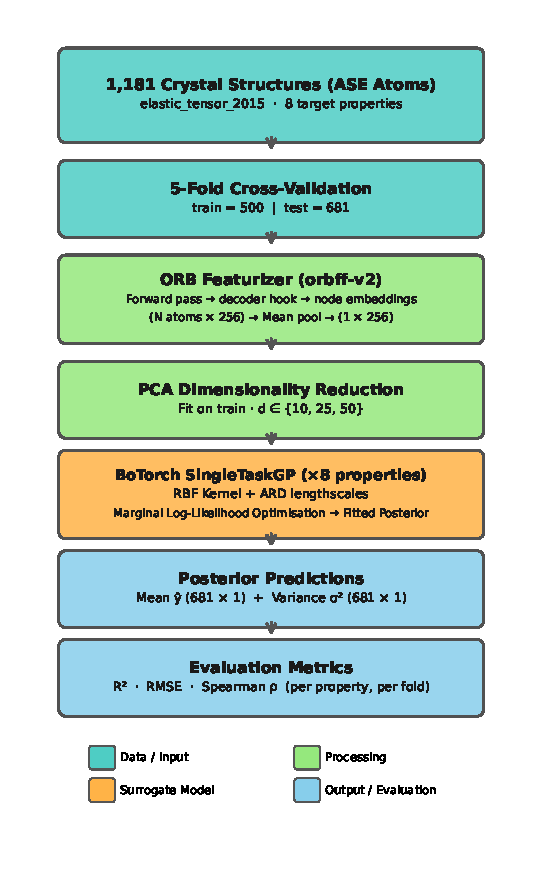
\includegraphics[width=\columnwidth]{figures/fig1_pipeline_schematic.pdf}
    \caption{Modular pipeline for foundation-model-based surrogate modelling. Crystal structures are featurised by one of four embedding methods (SOAP, MACE, ORB, UMA/eSEN), projected to lower dimensions via PCA, and fed into a probabilistic surrogate model (GP, MTGP, or DGP). Each component can be independently swapped, enabling systematic cross-factorial evaluation.}
    \label{fig:pipeline}
\end{figure}


\subsection{Datasets}
\label{sec:datasets}

We evaluate our pipeline on three publicly available datasets from the \texttt{matminer} library~\cite{ward2018matminer}, chosen to span a diverse range of materials properties: mechanical (elastic), electronic (dielectric), and vibrational (phonon).
Table~\ref{tab:datasets} summarises the key characteristics of each dataset.

\begin{table}[H]
    \centering
    \caption{Summary of the three benchmark datasets. All datasets are sourced from \texttt{matminer} and contain DFT-computed properties from the Materials Project~\cite{jain2013materials}.}
    \label{tab:datasets}
    \small
    \begin{tabular}{@{}llcc@{}}
        \toprule
        \textbf{Dataset} & \textbf{Property Type} & \textbf{Structures} & \textbf{Targets} \\
        \midrule
        \texttt{elastic\_tensor\_2015} & Mechanical & $\sim$1{,}181 & 8 \\
        \texttt{dielectric\_constant} & Electronic & $\sim$1{,}056 & 4 \\
        \texttt{phonon\_dielectric\_mp} & Phonon/Electronic & $\sim$1{,}296 & 3 \\
        \bottomrule
    \end{tabular}
\end{table}

\textbf{Elastic tensor dataset}~\cite{deJong2015elastic} contains 1{,}181 inorganic crystalline structures with DFT-computed elastic constants.
We predict 8~target properties: the Voigt, Voigt--Reuss--Hill (VRH), and Reuss averages of both bulk modulus ($K$) and shear modulus ($G$), together with elastic anisotropy and Poisson's ratio.
These properties range from ``easy'' (bulk modulus variants, which depend primarily on bond stiffness and local chemistry) to ``hard'' (elastic anisotropy, which requires capturing directional bonding and crystal symmetry).

\textbf{Dielectric constant dataset}~\cite{petousis2017high} contains approximately 1{,}056 structures with 4~target properties: band gap, refractive index ($n$), and the electronic and total components of the polycrystalline dielectric constant (\texttt{poly\_electronic} and \texttt{poly\_total}).
These properties are sensitive to electronic structure details that are only indirectly captured by geometric embeddings.

\textbf{Phonon dielectric dataset} from the Materials Project contains approximately 1{,}296 structures with 3~target properties: electronic and total dielectric constants (\texttt{eps\_electronic}, \texttt{eps\_total}) and the last phonon density of states peak (\texttt{last\_phdos\_peak}).
The dielectric constants prove extremely challenging for all methods (near-zero \Rtwo{}), while the phonon peak is moderately predictable.


\subsection{Featurizers}
\label{sec:featurizers}

We compare four featurisation strategies spanning the spectrum from classical hand-crafted descriptors to modern foundation model embeddings.
Table~\ref{tab:featurizers} summarises their key architectural differences.

\begin{table*}[!htb]
    \centering
    \caption{Comparison of the four featurisation methods. Foundation model embeddings (MACE, ORB, UMA/eSEN) are extracted from pre-trained models without fine-tuning. The raw embedding dimensionality is reduced via PCA before surrogate training.}
    \label{tab:featurizers}
    \small
    \begin{tabular}{@{}lllcl@{}}
        \toprule
        \textbf{Featurizer} & \textbf{Type} & \textbf{Pre-training Data} & \textbf{Raw Dim.} & \textbf{Key Reference} \\
        \midrule
        SOAP & Classical descriptor & None (analytical) & $\sim$1{,}000+ & Bart{\'o}k \emph{et al.}~\cite{bartok2013representing} \\
        MACE & Foundation model & MPTrj ($\sim$150k structs.) & $\sim$256 & Batatia \emph{et al.}~\cite{batatia2022mace,batatia2024foundation} \\
        ORB & Foundation model & Alexandria + MPTrj ($\sim$120M configs.) & $\sim$256 & Orbital Materials~\cite{orb2024} \\
        UMA/eSEN & Foundation model & Multiple sources & $\sim$256 & Meta FAIR~\cite{uma2025} \\
        \bottomrule
    \end{tabular}
\end{table*}

\textbf{SOAP} (Smooth Overlap of Atomic Positions)~\cite{bartok2013representing} is a classical descriptor that encodes local atomic environments as the power spectrum of a smooth atomic density expanded in radial basis functions and spherical harmonics.
We use the DScribe implementation~\cite{dscribe2020} with standard settings for inorganic crystals.
The structure-level descriptor is obtained by averaging over all atomic environments.
SOAP serves as the classical baseline: it sees only local neighbourhoods within a fixed cutoff radius, analogous to a pinhole camera that captures the immediate scene but misses the wider landscape.

\textbf{MACE}~\cite{batatia2022mace,batatia2024foundation} is an equivariant message-passing neural network that captures many-body interactions through higher-order tensor products.
We extract pooled node embeddings from the pre-trained MACE-MP-0 foundation model~\cite{batatia2024foundation}, which was trained on the MPTrj dataset of $\sim$150{,}000 structures from the Materials Project.
No fine-tuning is performed; the model is used purely as a feature extractor.

\textbf{ORB}~\cite{orb2024} is a graph neural network pre-trained by Orbital Materials on the combined Alexandria and MPTrj datasets, comprising approximately 120~million atomic configurations.
Its graph attention architecture with edge and node features is specifically tuned for periodic crystal structures.
We extract the final-layer embeddings and average over atomic sites.
ORB's large and chemically diverse pre-training corpus gives it broad coverage of the periodic table---analogous to a DSLR camera that captures the full scene with depth of field.

\textbf{UMA/eSEN} (Universal Materials Architecture)~\cite{uma2025} is Meta FAIR's universal interatomic potential based on the eSCN/eSEN architecture.
Pre-trained on multiple data sources spanning diverse chemistries, it represents the most recent generation of universal foundation models.
We extract embeddings analogously to MACE and ORB.


\subsection{Dimensionality Reduction}
\label{sec:pca}

Raw embeddings from all featurisers are projected to lower dimensions via PCA~\cite{jolliffe2002principal} before being passed to the surrogate model.
We evaluate three dimensionality levels: PCA\,=\,10, 25, and 50 components.
PCA serves two purposes: it reduces the computational cost of kernel evaluations in Gaussian processes (which scale cubically with input dimension) and mitigates collinearity among embedding features.
The PCA transformation is fitted on the training set and applied to the test set to prevent data leakage.


\subsection{Surrogate Models}
\label{sec:surrogates}

All surrogate models are implemented in BoTorch~\cite{balandat2020botorch}, built on GPyTorch~\cite{gardner2018gpytorch}, providing a unified framework for comparison.

\textbf{Gaussian Process (GP).}
We use the \texttt{SingleTaskGP} from BoTorch with a Mat{\'e}rn~5/2 kernel and automatic relevance determination (ARD).
Hyperparameters are optimised by maximising the marginal log-likelihood.
The GP is the workhorse of Bayesian optimisation: given a set of observations, it provides a closed-form posterior over the target function with calibrated uncertainty estimates~\cite{rasmussen2006gaussian}.
Each target property is modelled independently.

\textbf{Multi-Task GP (MTGP).}
We use the \texttt{MultiTaskGP} from BoTorch with the intrinsic coregionalisation model (ICM) kernel~\cite{bonilla2007multi}.
The ICM kernel decomposes the multi-output covariance as a Kronecker product of a task correlation matrix and a shared spatial kernel, allowing information to flow between related properties.
Think of it as building one amplifier that shares circuitry between the treble and bass channels, rather than building separate amplifiers for each.
The hypothesis is that correlated properties (e.g., $K_{\text{Voigt}}$, $K_{\text{VRH}}$, $K_{\text{Reuss}}$) should benefit from joint modelling.

\textbf{Deep GP (DGP).}
We use the \texttt{DeepGP} from BoTorch, a two-layer deep Gaussian process~\cite{damianou2013deep} trained via variational inference~\cite{dutordoir2021deep}.
The DGP stacks GP layers to capture non-linear input transformations that a single-layer GP cannot represent.
However, this additional expressiveness comes at the cost of more parameters, potentially more fragile training, and sensitivity to the input dimensionality.


\subsection{Experimental Protocol}
\label{sec:protocol}

We use 5-fold cross-validation with random splits.
For each dataset, we subsample training sets of size $\ntrain \in \{100, 250, 500\}$ from the training fold, while the test fold remains fixed.
This simulates the low-data regime typical of early-stage materials discovery campaigns where DFT calculations are expensive.

The full factorial design yields $4 \times 3 \times 3 \times 3 = 108$ configurations per dataset, times 3~datasets gives 324~configurations.
With 5-fold CV and per-property evaluation (8~properties for elastic, 4 for dielectric, 3 for phonon), the total number of individual model evaluations exceeds 8{,}640.

We report three complementary metrics:
\begin{itemize}[nosep]
    \item \textbf{\Rtwo{}} (coefficient of determination): measures the fraction of variance explained; penalises both bias and scatter.
    \item \textbf{RMSE} (root mean square error): measures absolute prediction error in the units of the target property.
    \item \textbf{Spearman rank correlation} ($\rho$): measures the monotonic relationship between predicted and true values; critical for Bayesian optimisation where we need to correctly \emph{rank} candidates rather than predict exact values.
\end{itemize}
All metrics are computed on the held-out test fold and averaged across folds.

\section{Results}
\label{sec:results}

We present results from 8{,}640 cross-validated experiments spanning three datasets, four featurisers, three surrogates, and three PCA dimensionalities.
Unless stated otherwise, all numbers refer to $\ntrain = 500$.

\subsection{Featurizer Ranking Across Datasets}
\label{sec:featurizer_ranking}

Figure~\ref{fig:bar_r2_all} presents bar charts of averaged \Rtwo{} for all featuriser--surrogate combinations across the three datasets.
ORB embeddings consistently rank first on every dataset and every surrogate.

\begin{figure*}[!htb]
    \centering
    \begin{subfigure}[t]{0.32\textwidth}
        \centering
        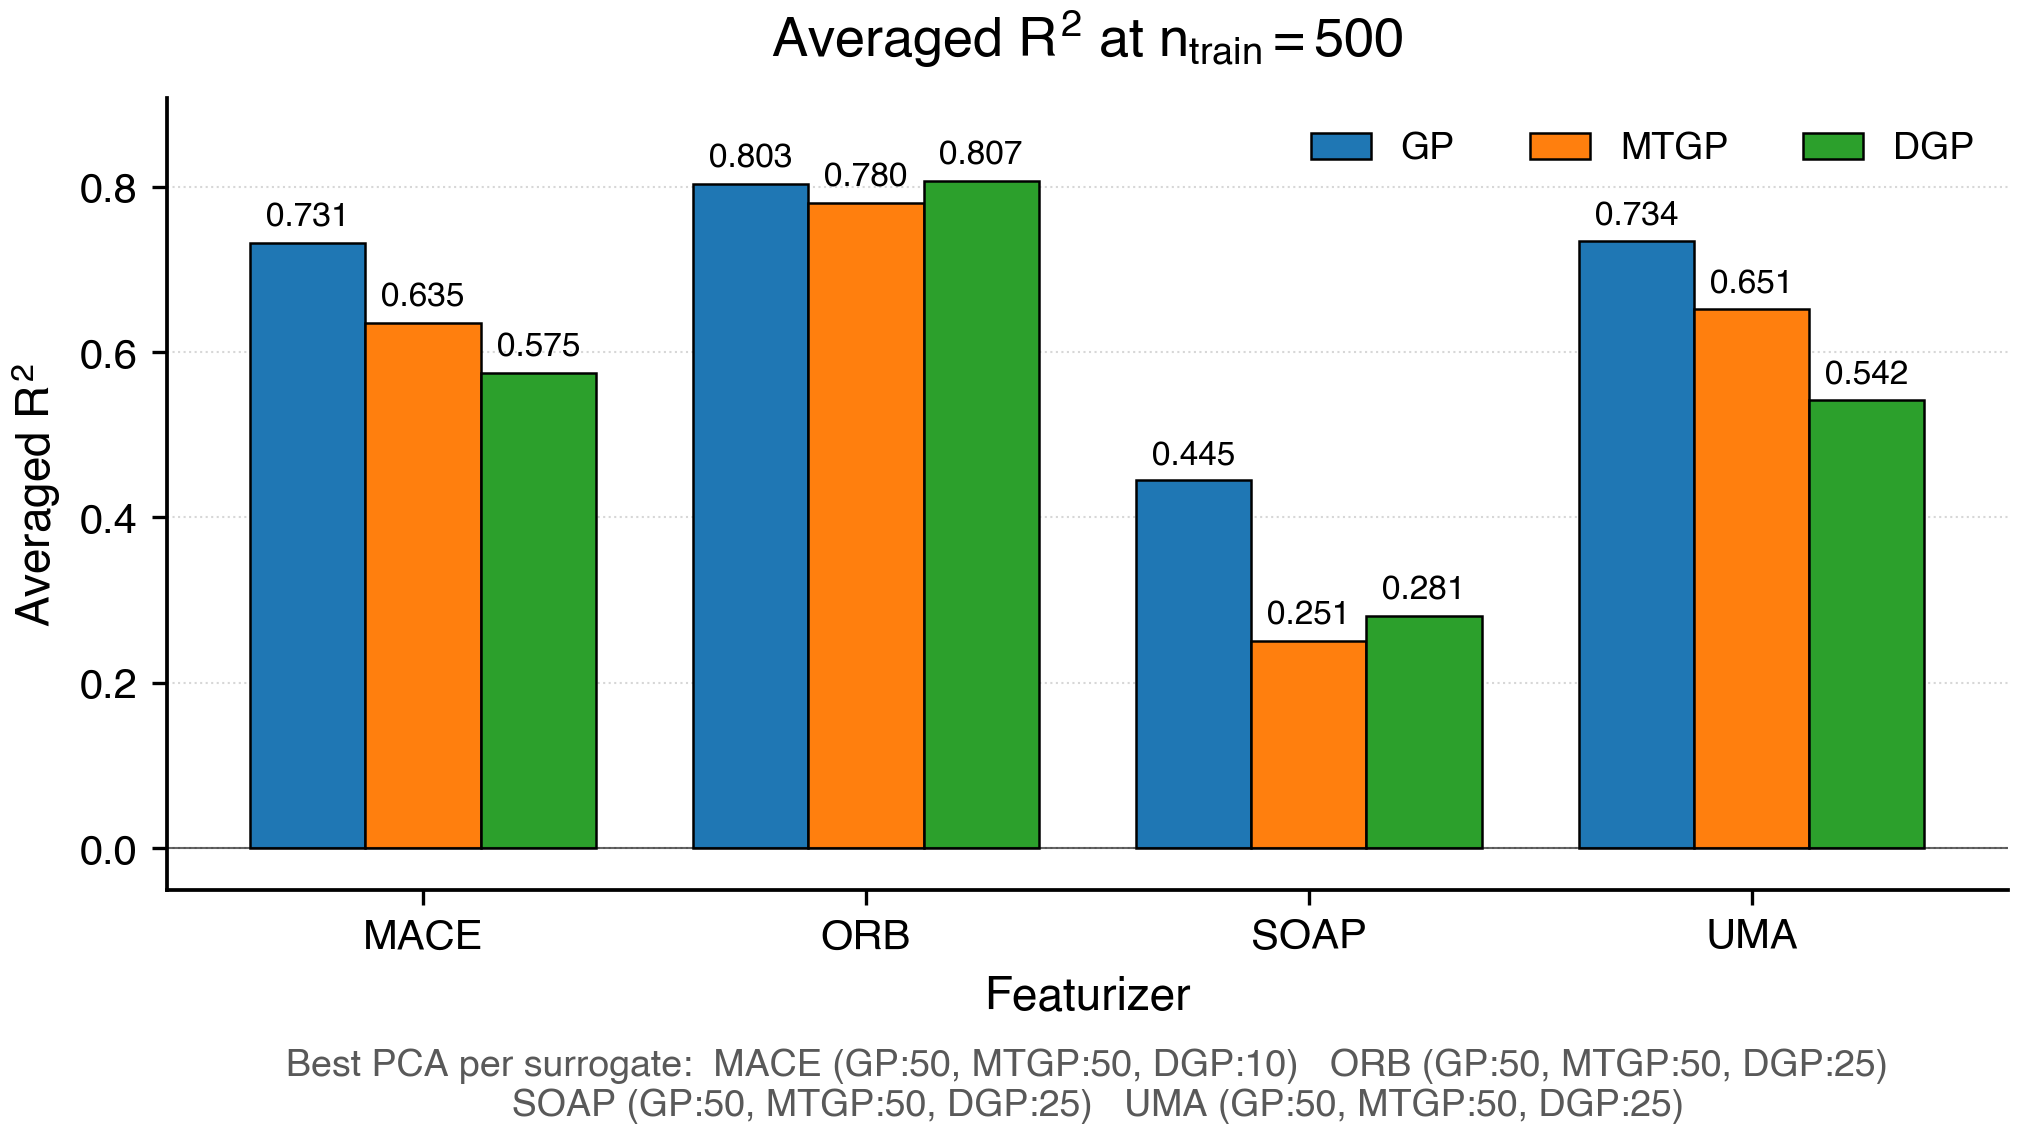
\includegraphics[width=\textwidth]{figures/fig2_bar_elastic_R2_grouped.png}
        \caption{Elastic tensor (8 properties)}
        \label{fig:bar_elastic}
    \end{subfigure}
    \hfill
    \begin{subfigure}[t]{0.32\textwidth}
        \centering
        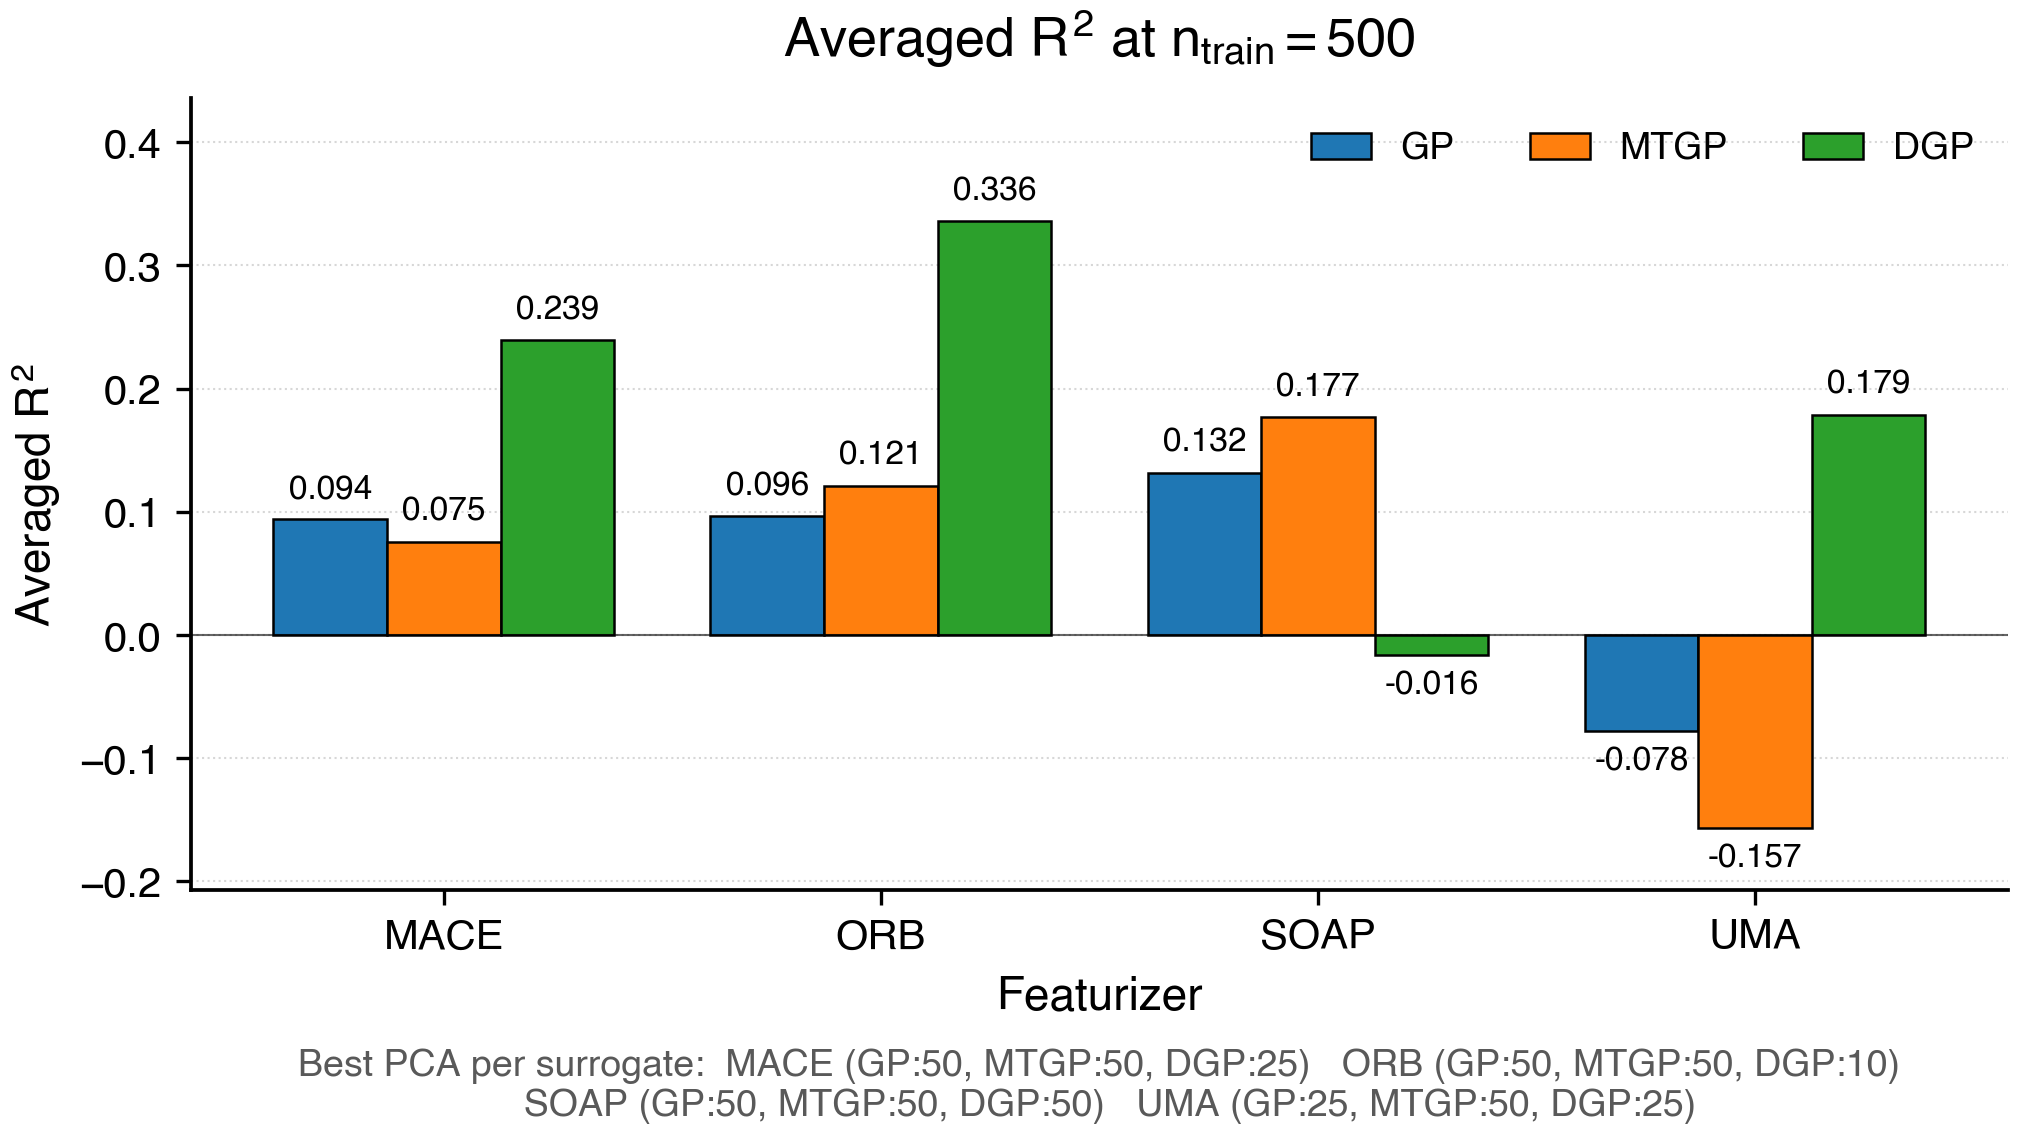
\includegraphics[width=\textwidth]{figures/fig2_bar_dielectric_R2_grouped.png}
        \caption{Dielectric constant (4 properties)}
        \label{fig:bar_dielectric}
    \end{subfigure}
    \hfill
    \begin{subfigure}[t]{0.32\textwidth}
        \centering
        
\includegraphics[width=\textwidth]{figures/fig2_bar_phonon_R2_grouped.png}
        \caption{Phonon dielectric (3 properties)}
        \label{fig:bar_phonon}
    \end{subfigure}
    \caption{Averaged \Rtwo{} across all target properties at $\ntrain = 500$, grouped by featuriser and surrogate model, for each of the three benchmark datasets. ORB embeddings dominate on all datasets. Note the different $y$-axis scales reflecting the vastly different prediction difficulty across domains.}
    \label{fig:bar_r2_all}
\end{figure*}

Table~\ref{tab:best_configs_elastic} reports the best configuration per featuriser--surrogate pair on the elastic tensor dataset.
The best overall configuration is ORB\,+\,DGP at PCA\,=\,25, achieving an averaged \Rtwo{} of 0.807 across all 8~elastic properties.
ORB\,+\,GP at PCA\,=\,50 is a close second at 0.803, with the critical advantage of far greater stability (Section~\ref{sec:pca_sensitivity}).
The featuriser ranking is remarkably consistent: ORB~($\bar{R}^2 \approx 0.80$) $>$ UMA~($\approx 0.73$) $\approx$ MACE~($\approx 0.73$) $\gg$ SOAP~($\approx 0.44$) for GP, with similar orderings for MTGP and DGP.

\begin{table*}[!htb]
    \centering
    \caption{Best configuration per featuriser--surrogate pair on the elastic tensor dataset ($\ntrain = 500$). For each combination, we report the PCA dimensionality that maximises averaged \Rtwo{} across all 8~properties, together with the corresponding averaged RMSE and Spearman~$\rho$.}
    \label{tab:best_configs_elastic}
    \small
    \begin{tabular}{@{}llcccc@{}}
        \toprule
        \textbf{Surrogate} & \textbf{Featurizer} & \textbf{Best PCA} & \textbf{Avg.\ \Rtwo{}} & \textbf{Avg.\ RMSE} & \textbf{Avg.\ Spearman} \\
        \midrule
        \multirow{4}{*}{GP}
        & ORB     & 50 & \textbf{0.803} & \textbf{17.37} & \textbf{0.842} \\
        & UMA     & 50 & 0.734 & 21.42 & 0.811 \\
        & MACE    & 50 & 0.731 & 20.46 & 0.820 \\
        & SOAP    & 50 & 0.445 & 33.63 & 0.688 \\
        \midrule
        \multirow{4}{*}{MTGP}
        & ORB     & 50 & \textbf{0.780} & \textbf{19.30} & \textbf{0.843} \\
        & UMA     & 50 & 0.651 & 25.80 & 0.780 \\
        & MACE    & 50 & 0.635 & 25.76 & 0.758 \\
        & SOAP    & 50 & 0.251 & 41.34 & 0.529 \\
        \midrule
        \multirow{4}{*}{DGP}
        & ORB     & 25 & \textbf{0.807} & \textbf{17.84} & \textbf{0.826} \\
        & MACE    & 10 & 0.575 & 25.53 & 0.659 \\
        & UMA     & 25 & 0.542 & 26.80 & 0.696 \\
        & SOAP    & 25 & 0.281 & 38.78 & 0.521 \\
        \bottomrule
    \end{tabular}
\end{table*}

Tables~\ref{tab:best_configs_dielectric} and~\ref{tab:best_configs_phonon} present the equivalent results for the dielectric and phonon datasets.
On the dielectric dataset, overall \Rtwo{} values are substantially lower, reflecting the difficulty of predicting electronic properties from geometric embeddings.
The best configuration is DGP\,+\,ORB at PCA\,=\,10 ($\bar{R}^2 = 0.336$, $\bar{\rho} = 0.778$).
Notably, SOAP is competitive on this dataset (MTGP\,+\,SOAP achieves $\bar{R}^2 = 0.177$), suggesting that the classical descriptor captures some local chemistry information relevant to dielectric response that foundation model embeddings emphasise less.

\begin{table}[H]
    \centering
    \caption{Best configuration per featuriser--surrogate pair on the dielectric constant dataset ($\ntrain = 500$).}
    \label{tab:best_configs_dielectric}
    \footnotesize
    \begin{tabular}{@{}llcccc@{}}
        \toprule
        \textbf{Surr.} & \textbf{Feat.} & \textbf{PCA} & \textbf{\Rtwo{}} & \textbf{RMSE} & \textbf{$\rho$} \\
        \midrule
        \multirow{4}{*}{GP}
        & SOAP    & 50 & 0.132 & 7.60 & 0.549 \\
        & ORB     & 50 & 0.096 & 7.84 & \textbf{0.746} \\
        & MACE    & 50 & 0.094 & 7.94 & 0.695 \\
        & UMA     & 25 & $-$0.078 & 8.14 & 0.609 \\
        \midrule
        \multirow{4}{*}{MTGP}
        & SOAP    & 50 & \textbf{0.177} & \textbf{7.27} & 0.583 \\
        & ORB     & 50 & 0.121 & 7.85 & \textbf{0.773} \\
        & MACE    & 50 & 0.075 & 7.90 & 0.715 \\
        & UMA     & 50 & $-$0.157 & 8.49 & 0.656 \\
        \midrule
        \multirow{4}{*}{DGP}
        & ORB     & 10 & \textbf{0.336} & \textbf{6.88} & \textbf{0.778} \\
        & MACE    & 25 & 0.239 & 7.31 & 0.754 \\
        & UMA     & 25 & 0.179 & 7.35 & 0.742 \\
        & SOAP    & 50 & $-$0.016 & 7.46 & 0.019 \\
        \bottomrule
    \end{tabular}
\end{table}

\begin{table}[H]
    \centering
    \caption{Best configuration per featuriser--surrogate pair on the phonon dielectric dataset ($\ntrain = 500$). RMSE omitted; values dominated by extreme dielectric constant outliers.}
    \label{tab:best_configs_phonon}
    \footnotesize
    \begin{tabular}{@{}llccc@{}}
        \toprule
        \textbf{Surr.} & \textbf{Feat.} & \textbf{PCA} & \textbf{\Rtwo{}} & \textbf{$\rho$} \\
        \midrule
        \multirow{4}{*}{GP}
        & ORB     & 50 & \textbf{0.303} & \textbf{0.824} \\
        & UMA     & 50 & 0.272 & 0.756 \\
        & MACE    & 50 & 0.269 & 0.719 \\
        & SOAP    & 50 & 0.235 & 0.639 \\
        \midrule
        \multirow{4}{*}{MTGP}
        & ORB     & 25 & \textbf{0.302} & \textbf{0.830} \\
        & MACE    & 50 & 0.267 & 0.743 \\
        & UMA     & 50 & 0.265 & 0.806 \\
        & SOAP    & 50 & 0.239 & 0.700 \\
        \midrule
        \multirow{4}{*}{DGP}
        & ORB     & 25 & \textbf{0.302} & \textbf{0.807} \\
        & UMA     & 25 & 0.258 & 0.664 \\
        & SOAP    & 25 & 0.212 & 0.599 \\
        & MACE    & 10 & 0.200 & 0.635 \\
        \bottomrule
    \end{tabular}
\end{table}

On the phonon dataset, the gap between featurisers is smaller.
ORB\,+\,GP achieves $\bar{R}^2 = 0.303$ and $\bar{\rho} = 0.824$, but SOAP is only 0.07 \Rtwo{} points behind.
This reduced gap is because two of the three phonon properties (eps\_electronic and eps\_total) yield near-zero \Rtwo{} for \emph{all} methods, compressing the averaged \Rtwo{} range.
On the one well-predicted property (last phonon DOS peak), the ORB advantage is pronounced: $R^2 = 0.911$ vs.\ SOAP's 0.708.
The MTGP shows its best relative performance on this dataset, with ORB\,+\,MTGP ($\bar{\rho} = 0.830$) essentially matching the GP ($\bar{\rho} = 0.824$).

\FloatBarrier
\subsection{Surrogate Model Comparison}
\label{sec:surrogate_comparison}

Figure~\ref{fig:heatmap_all} presents heatmaps of all featuriser--surrogate--PCA combinations at $\ntrain = 500$ for each dataset.

\begin{figure*}[!htb]
    \centering
    \begin{subfigure}[t]{0.32\textwidth}
        \centering
        
\includegraphics[width=\textwidth]{figures/fig3_heatmap_R2_n500.pdf}
        \caption{Elastic tensor}
        \label{fig:heatmap_elastic}
    \end{subfigure}
    \hfill
    \begin{subfigure}[t]{0.32\textwidth}
        \centering
        
\includegraphics[width=\textwidth]{figures/fig_heatmap_dielectric_R2_n500.pdf}
        \caption{Dielectric constant}
        \label{fig:heatmap_dielectric}
    \end{subfigure}
    \hfill
    \begin{subfigure}[t]{0.32\textwidth}
        \centering
        
\includegraphics[width=\textwidth]{figures/fig_heatmap_phonon_R2_n500.pdf}
        \caption{Phonon dielectric}
        \label{fig:heatmap_phonon}
    \end{subfigure}
    \caption{Heatmaps of averaged \Rtwo{} for each featuriser--surrogate combination at $\ntrain = 500$ across all three datasets. Rows represent descriptor--PCA combinations; columns represent surrogate models. The DGP column shows a stark bimodal pattern across all datasets: strong at low PCA, catastrophic at PCA\,=\,50.}
    \label{fig:heatmap_all}
\end{figure*}

The GP is the most reliable surrogate across all three datasets and all featuriser--PCA configurations.
It achieves the best or near-best \Rtwo{} in the majority of settings and exhibits the lowest cross-fold variance.
On the elastic dataset, GP\,+\,ORB at PCA\,=\,50 reaches $\bar{R}^2 = 0.803$ with $\bar{\rho} = 0.842$---the highest ranking accuracy of any stable configuration.

The MTGP shows mixed results.
On the elastic dataset, it consistently underperforms the independent GP: MTGP\,+\,ORB achieves $\bar{R}^2 = 0.780$ versus the GP's 0.803.
On the phonon dataset, however, MTGP is essentially tied with the GP ($\bar{R}^2 = 0.302$ vs.\ 0.303; $\bar{\rho} = 0.830$ vs.\ 0.824), with the correlation between eps\_electronic, eps\_total, and the phonon DOS peak providing some multi-task signal.
On the dielectric dataset, MTGP\,+\,SOAP surprisingly leads the GP in \Rtwo{} (0.177 vs.\ 0.132), suggesting that multi-task learning can compensate for weaker featurisers when property correlations are strong.

The DGP exhibits a dramatic split personality across all three datasets.
On the elastic data, ORB\,+\,DGP at PCA\,=\,25 achieves the single best \Rtwo{} ($0.807$), but collapses to $-0.017$ at PCA\,=\,50.
On the dielectric data, DGP\,+\,ORB at PCA\,=\,10 achieves the best \Rtwo{} ($0.336$), substantially outperforming GP and MTGP---but only at low dimensionality.
On the phonon data, a similar pattern holds: DGP\,+\,ORB at PCA\,=\,25 matches the GP ($\bar{R}^2 = 0.302$) but fails at PCA\,=\,50.
This extreme fragility (Section~\ref{sec:pca_sensitivity}) makes the DGP unsuitable as a default choice despite its occasional peak performance.

\FloatBarrier
\subsection{PCA Sensitivity Analysis}
\label{sec:pca_sensitivity}

Figure~\ref{fig:pca_all} reveals markedly different PCA sensitivity profiles across surrogates, featurisers, and datasets.

\begin{figure*}[!htb]
    \centering
    \begin{subfigure}[t]{0.32\textwidth}
        \centering
        
\includegraphics[width=\textwidth]{figures/fig4_pca_sensitivity_n500.pdf}
        \caption{Elastic tensor}
        \label{fig:pca_elastic}
    \end{subfigure}
    \hfill
    \begin{subfigure}[t]{0.32\textwidth}
        \centering
        
\includegraphics[width=\textwidth]{figures/fig_pca_dielectric_R2_n500.pdf}
        \caption{Dielectric constant}
        \label{fig:pca_dielectric}
    \end{subfigure}
    \hfill
    \begin{subfigure}[t]{0.32\textwidth}
        \centering
        
\includegraphics[width=\textwidth]{figures/fig_pca_phonon_R2_n500.pdf}
        \caption{Phonon dielectric}
        \label{fig:pca_phonon}
    \end{subfigure}
    \caption{Effect of PCA dimensionality on averaged \Rtwo{} at $\ntrain = 500$ across all three datasets. GP and MTGP show monotonic improvement or robustness as PCA increases. DGP (dashed lines) exhibits catastrophic failure at PCA\,=\,50 across all datasets.}
    \label{fig:pca_all}
\end{figure*}

For the GP, all featurisers show monotonic improvement as PCA increases from 10 to 50 on the elastic dataset.
ORB's GP performance improves from 0.736 (PCA\,=\,10) to 0.803 (PCA\,=\,50), a modest but consistent gain.
SOAP benefits the most: its $\bar{R}^2$ more than doubles from 0.197 (PCA\,=\,10) to 0.445 (PCA\,=\,50), reflecting the high intrinsic dimensionality of the SOAP descriptor.
MACE is the most PCA-robust featuriser on the elastic data, varying by only $\Delta R^2 = 0.005$ across PCA levels (0.727 to 0.731).

The same qualitative pattern holds on the dielectric and phonon datasets, though with smaller absolute improvements.
On the phonon data, GP\,+\,ORB improves from $\bar{R}^2 = 0.281$ (PCA\,=\,10) to $0.303$ (PCA\,=\,50).
On the dielectric data, SOAP\,+\,GP shows the most improvement from PCA\,=\,10 ($-0.078$) to PCA\,=\,50 ($0.132$), again indicating that SOAP's useful information is spread across many principal components.

The DGP's catastrophic failure at PCA\,=\,50 is universal across datasets.
On the elastic data, ORB\,+\,DGP drops from 0.807 (PCA\,=\,25) to $-0.017$ (PCA\,=\,50).
On the dielectric data, ORB\,+\,DGP drops from 0.236 (PCA\,=\,25) to $-0.022$ (PCA\,=\,50).
On the phonon data, ORB\,+\,DGP drops from 0.302 (PCA\,=\,25) to $-0.002$ (PCA\,=\,50).
The consistency of this collapse across three very different property domains confirms that it is a fundamental limitation of the variational DGP inference at these sample sizes, not a property-specific artefact.

\FloatBarrier
\subsection{Learning Curves}
\label{sec:learning_curves}

Figure~\ref{fig:learning_curves} presents learning curves for the elastic tensor dataset, the only dataset for which we have results at all three training sizes ($\ntrain \in \{100, 250, 500\}$).

\begin{figure}[H]
    \centering
    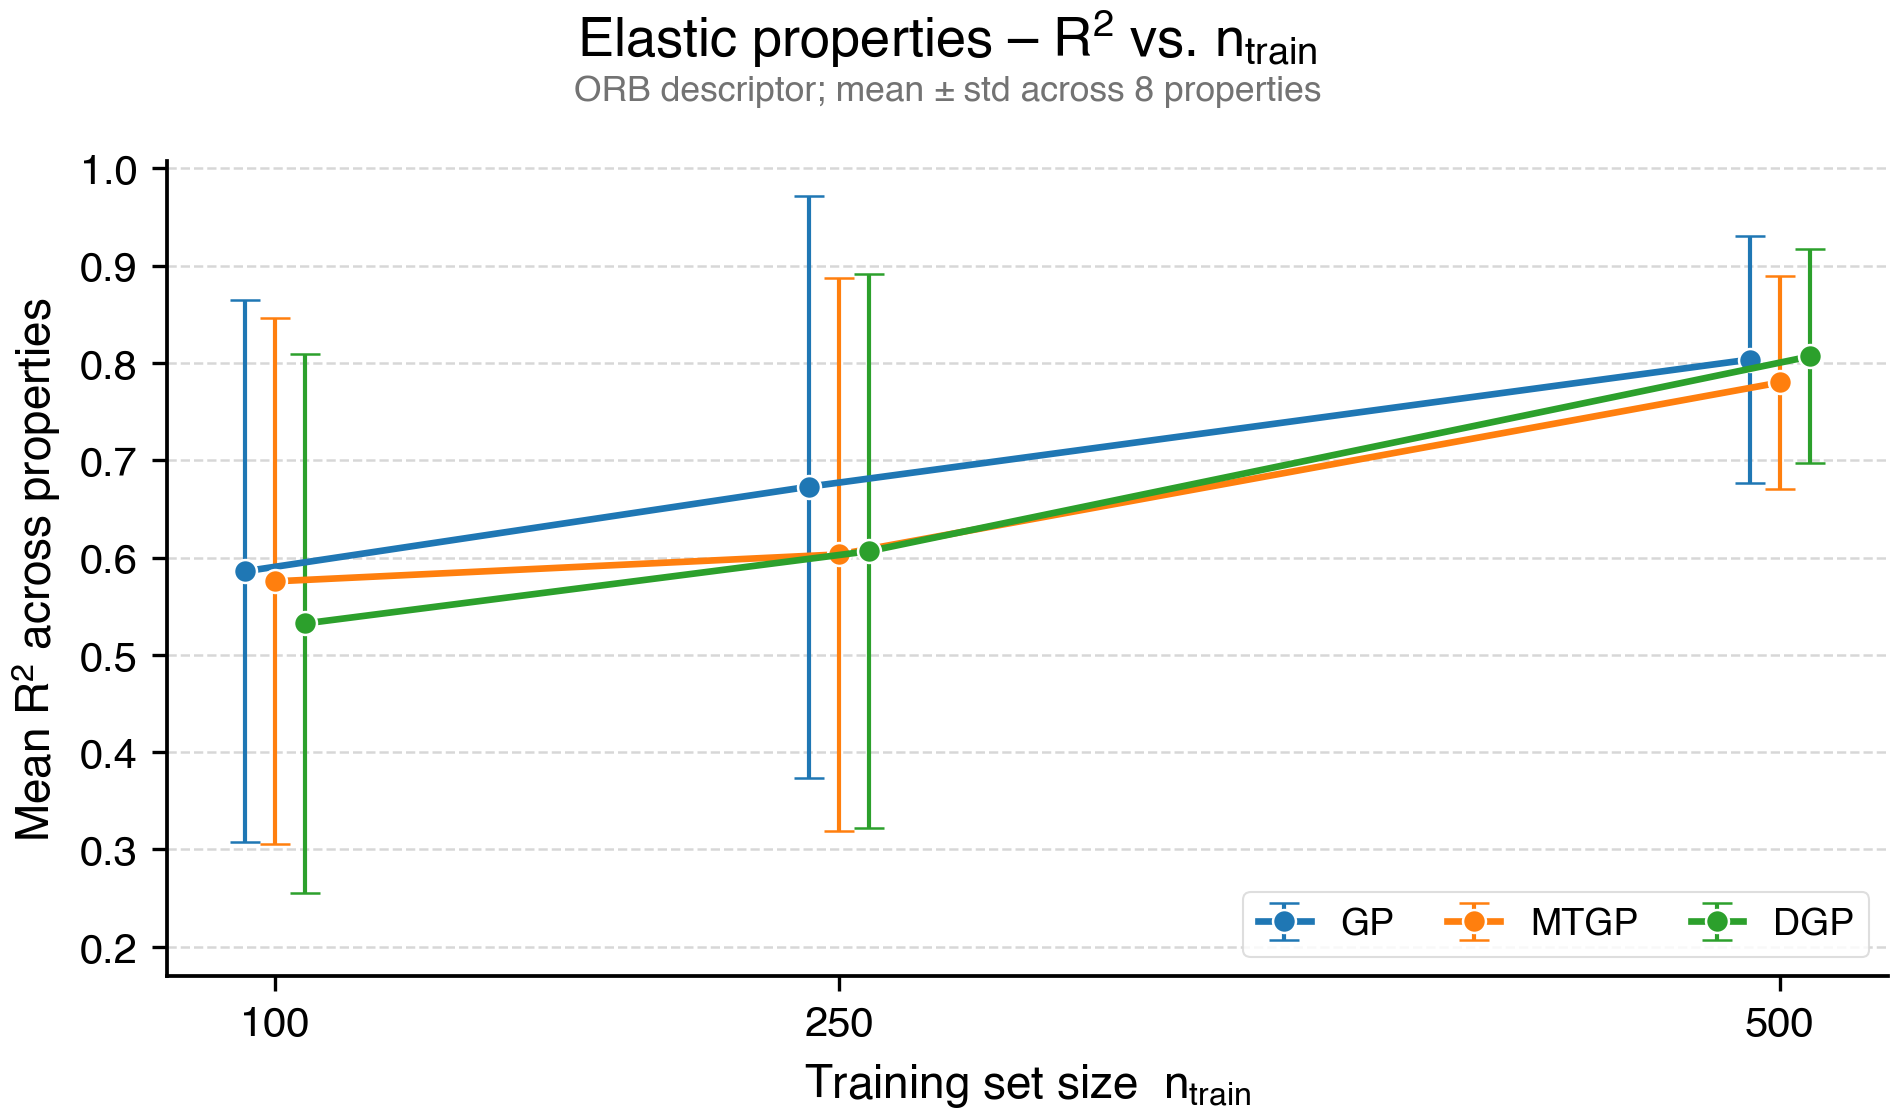
\includegraphics[width=\columnwidth]{figures/fig5_learning_curve_R2.png}
    \caption{Learning curves showing averaged \Rtwo{} as a function of training set size for all featuriser--surrogate combinations on the elastic tensor dataset. ORB\,+\,GP at $\ntrain = 100$ approaches the performance of SOAP\,+\,GP at $\ntrain = 500$.}
    \label{fig:learning_curves}
\end{figure}

\begin{table}[H]
    \centering
    \caption{Learning curve summary for ORB embeddings across all three surrogates on the elastic tensor dataset. \Rtwo{} values are averaged across all 8~elastic properties at the best PCA setting for each configuration.}
    \label{tab:learning_curves}
    \small
    \begin{tabular}{@{}lcccc@{}}
        \toprule
        \textbf{Surrogate} & $\ntrain{=}100$ & $\ntrain{=}250$ & $\ntrain{=}500$ & \textbf{Gain} \\
        \midrule
        GP  & 0.535 & 0.687 & 0.803 & +50\% \\
        MTGP & 0.530 & 0.627 & 0.780 & +47\% \\
        DGP  & 0.487 & 0.641 & 0.807 & +66\% \\
        \bottomrule
    \end{tabular}
\end{table}

ORB embeddings exhibit remarkable data efficiency.
At $\ntrain = 100$, ORB\,+\,GP already achieves $\bar{R}^2 \approx 0.535$ on the elastic tensor properties---surpassing SOAP\,+\,GP at $\ntrain = 500$ ($\bar{R}^2 = 0.445$).
The foundation model embeddings effectively provide a ``head start'' equivalent to $\sim$400 additional training samples.

The learning curves also reveal that the GP and DGP converge at different rates.
The GP shows the most consistent improvement from $\ntrain = 100$ to 500, gaining +50\% in \Rtwo{}.
The DGP shows the largest relative gain (+66\%) but starts lower at $\ntrain = 100$ due to insufficient data for variational training.
The MTGP shows the weakest scaling, plateauing earlier than the independent GP.
These results imply that in ultra-low-data campaigns ($\ntrain < 100$), the GP is the clear choice; the DGP requires at least $\sim$250 samples to match the GP.

\subsubsection{Dielectric and Phonon Learning Curves}
\label{sec:learning_curves_dielectric_phonon}

Learning curves for the dielectric and phonon datasets reveal markedly different scaling behaviour from the elastic case.
Figure~\ref{fig:learning_curves_dielectric} presents the averaged \Rtwo{} and Spearman correlation as a function of training set size for the dielectric constant dataset.
Unlike the elastic dataset, where all surrogates improve monotonically with data, the dielectric dataset shows that GP and MTGP \Rtwo{} values \emph{decrease} from $\ntrain = 100$ to $\ntrain = 500$, while the DGP remains relatively stable.
This counterintuitive behaviour reflects the heavy-tailed property distributions (polycrystalline dielectric constants span orders of magnitude): as the training set grows, it includes more extreme outliers that dominate the squared-error metric.
The Spearman correlations, by contrast, are stable or improve, confirming that the surrogates maintain their ranking capability even as absolute prediction degrades.

\begin{figure}[H]
    \centering
    \begin{subfigure}[t]{0.48\columnwidth}
        \centering
        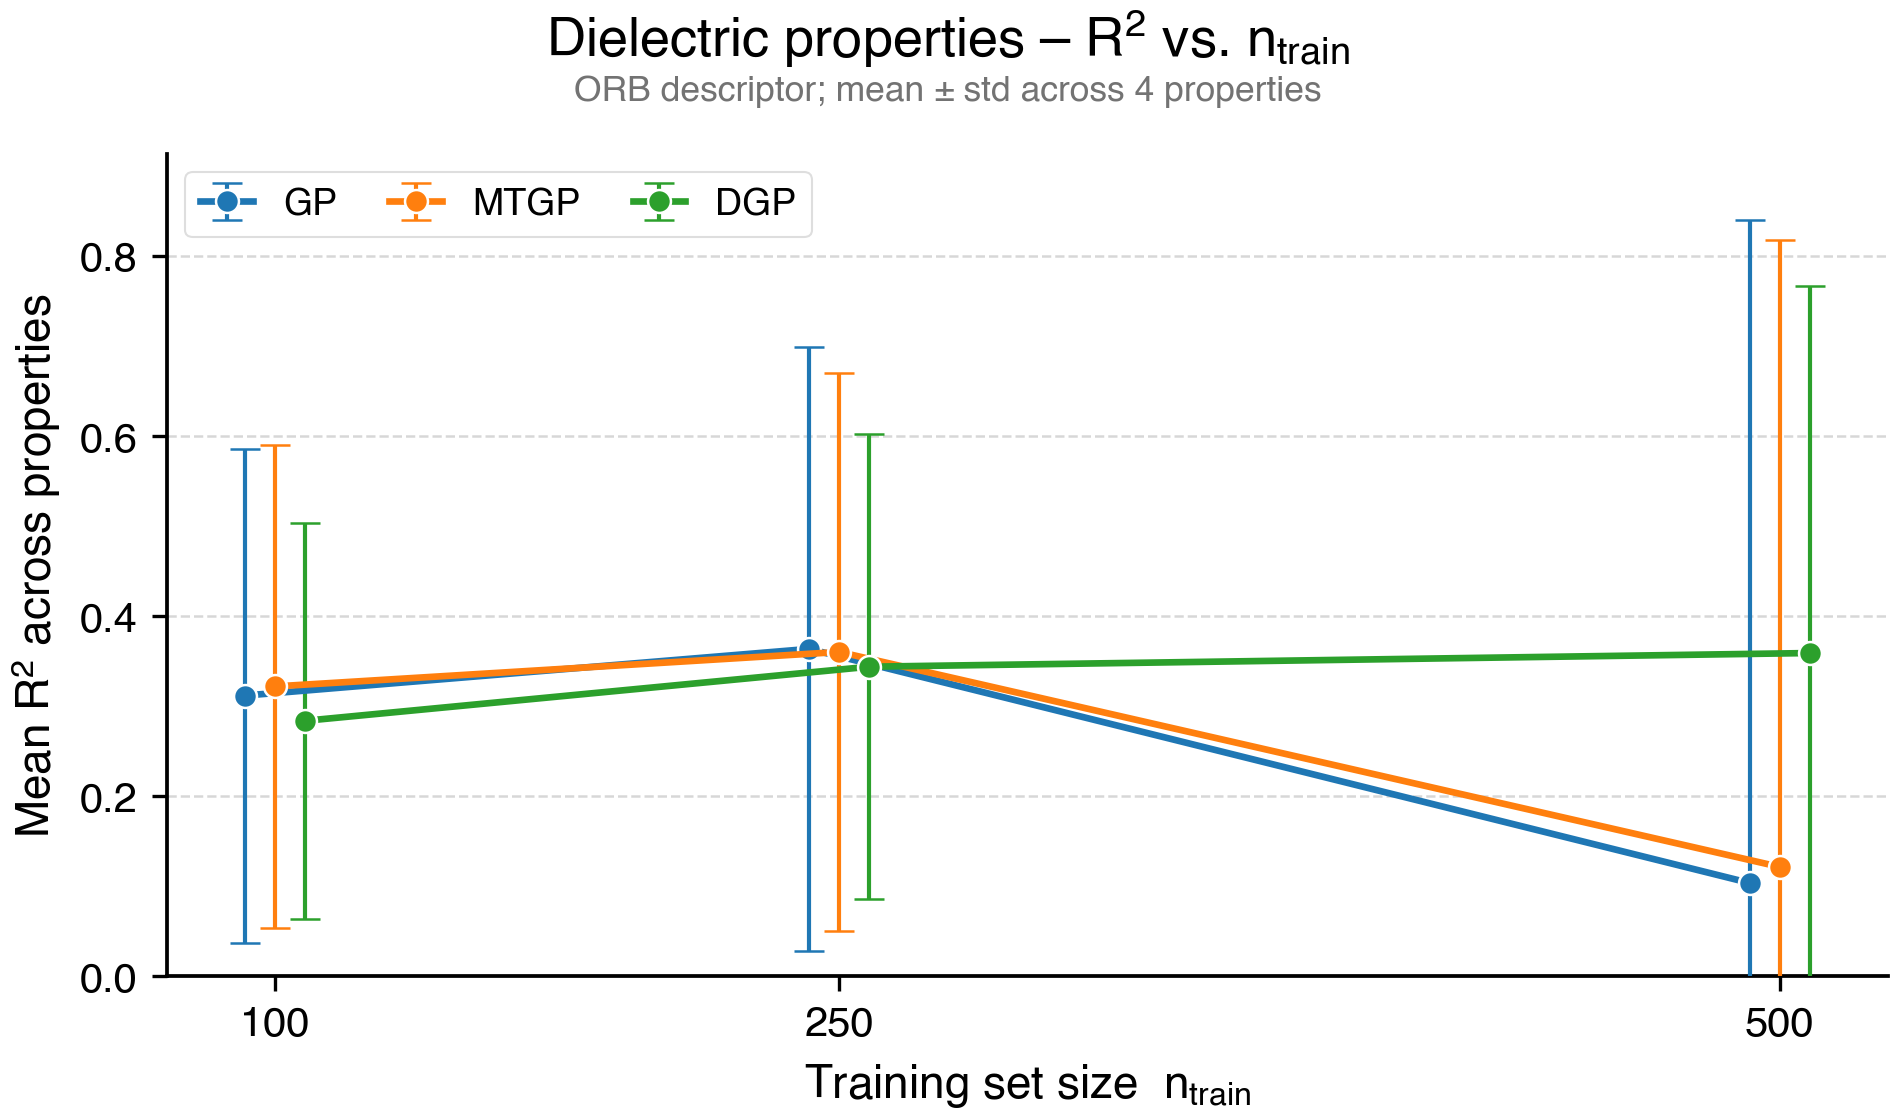
\includegraphics[width=\textwidth]{figures/fig_combined_dielectric_R2_learning_curve.png}
        \caption{Averaged \Rtwo{}}
        \label{fig:lc_dielectric_r2}
    \end{subfigure}
    \hfill
    \begin{subfigure}[t]{0.48\columnwidth}
        \centering
        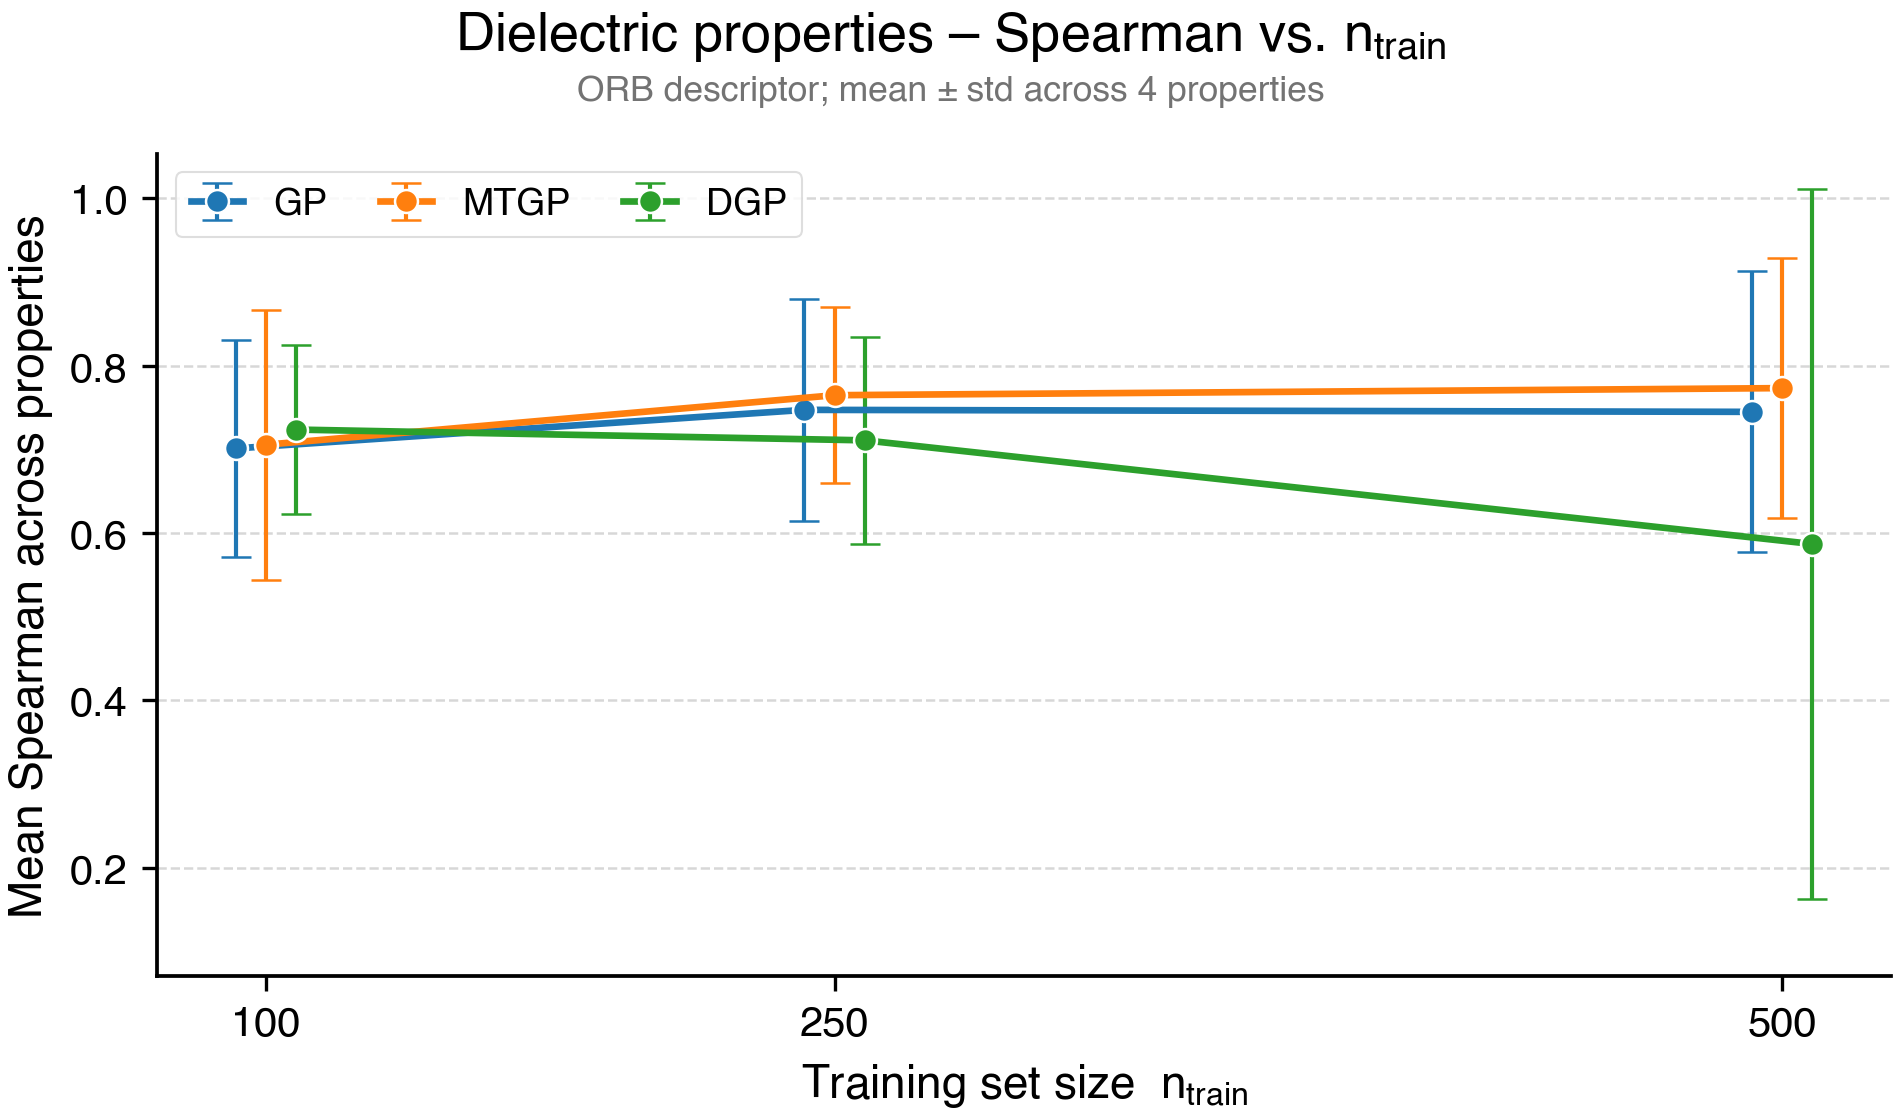
\includegraphics[width=\textwidth]{figures/fig_combined_dielectric_Spearman_learning_curve.png}
        \caption{Averaged Spearman $\rho$}
        \label{fig:lc_dielectric_spearman}
    \end{subfigure}
    \caption{Learning curves for the dielectric constant dataset (ORB descriptor, best PCA per surrogate). GP and MTGP \Rtwo{} values decrease with training size due to heavy-tailed property distributions, while Spearman correlations remain stable, reinforcing the finding that ranking accuracy is more robust than regression accuracy for electronically complex properties.}
    \label{fig:learning_curves_dielectric}
\end{figure}

Figure~\ref{fig:learning_curves_phonon} shows the analogous learning curves for the phonon dielectric dataset.
Here, all three surrogates show modest improvement with training size, and the DGP achieves the best \Rtwo{} at $\ntrain = 500$---consistent with its ability to model non-linear structure--property relationships given sufficient data.
The large error bars on the DGP reflect its sensitivity to the random initialisation of variational parameters, a practical consideration for reproducibility.
Spearman correlations for the phonon dataset improve steadily, with MTGP achieving the highest ranking accuracy at $\ntrain = 500$, consistent with the multi-task signal from correlated dielectric properties.

\begin{figure}[H]
    \centering
    \begin{subfigure}[t]{0.48\columnwidth}
        \centering
        
\includegraphics[width=\textwidth]{figures/fig_combined_phonon_R2_learning_curve.png}
        \caption{Averaged \Rtwo{}}
        \label{fig:lc_phonon_r2}
    \end{subfigure}
    \hfill
    \begin{subfigure}[t]{0.48\columnwidth}
        \centering
        
\includegraphics[width=\textwidth]{figures/fig_combined_phonon_Spearman_learning_curve.png}
        \caption{Averaged Spearman $\rho$}
        \label{fig:lc_phonon_spearman}
    \end{subfigure}
    \caption{Learning curves for the phonon dielectric dataset (ORB descriptor, best PCA per surrogate). All surrogates show modest improvement with training size. DGP achieves the best \Rtwo{} at $\ntrain = 500$ but with large variance. MTGP shows the strongest Spearman scaling, reaching $\bar{\rho} > 0.83$ at $\ntrain = 500$.}
    \label{fig:learning_curves_phonon}
\end{figure}

The contrasting learning curve behaviours across the three datasets reveal a key insight: the standard ``more data always helps'' intuition holds for geometric properties (elastic) and vibrational properties (phonon), but breaks down for electronic properties (dielectric) when measured by \Rtwo{}.
This dataset-dependent scaling further supports our recommendation to use Spearman correlation as the primary evaluation metric for surrogates targeting Bayesian optimisation.

\FloatBarrier
\subsection{Per-Property Difficulty Analysis}
\label{sec:property_analysis}

Not all properties are created equal.
Figure~\ref{fig:difficulty_all} presents property difficulty matrices for all three datasets, and the radar charts in Figure~\ref{fig:radar_all} visualise ORB's per-property profile.

\begin{figure*}[!htb]
    \centering
    \begin{subfigure}[t]{0.32\textwidth}
        \centering
        
\includegraphics[width=\textwidth]{figures/fig6_property_difficulty.pdf}
        \caption{Elastic tensor}
        \label{fig:diff_elastic}
    \end{subfigure}
    \hfill
    \begin{subfigure}[t]{0.32\textwidth}
        \centering
        
\includegraphics[width=\textwidth]{figures/fig_difficulty_dielectric_n500.pdf}
        \caption{Dielectric constant}
        \label{fig:diff_dielectric}
    \end{subfigure}
    \hfill
    \begin{subfigure}[t]{0.32\textwidth}
        \centering
        
\includegraphics[width=\textwidth]{figures/fig_difficulty_phonon_n500.pdf}
        \caption{Phonon dielectric}
        \label{fig:diff_phonon}
    \end{subfigure}
    \caption{Property difficulty matrices showing the best-achievable \Rtwo{} per property across all featuriser--PCA combinations at $\ntrain = 500$, broken down by surrogate model. (a)~Elastic: bulk modulus variants are easiest; anisotropy and Poisson's ratio are hardest. (b)~Dielectric: band gap is easiest; polycrystalline dielectric constants are hardest. (c)~Phonon: last phonon DOS peak is well predicted; dielectric constants are essentially unpredictable.}
    \label{fig:difficulty_all}
\end{figure*}

\begin{figure*}[!htb]
    \centering
    \begin{subfigure}[t]{0.32\textwidth}
        \centering
        
\includegraphics[width=\textwidth]{figures/fig7_radar_orb_R2.pdf}
        \caption{Elastic tensor}
        \label{fig:radar_elastic}
    \end{subfigure}
    \hfill
    \begin{subfigure}[t]{0.32\textwidth}
        \centering
        
\includegraphics[width=\textwidth]{figures/fig_radar_dielectric_orb_R2_n500.pdf}
        \caption{Dielectric constant}
        \label{fig:radar_dielectric}
    \end{subfigure}
    \hfill
    \begin{subfigure}[t]{0.32\textwidth}
        \centering
        
\includegraphics[width=\textwidth]{figures/fig_radar_phonon_orb_R2_n500.pdf}
        \caption{Phonon dielectric}
        \label{fig:radar_phonon}
    \end{subfigure}
    \caption{Radar charts showing ORB's per-property \Rtwo{} across GP, MTGP, and DGP at $\ntrain = 500$ for each dataset. The elastic dataset shows the most uniform performance across properties; the dielectric and phonon datasets exhibit extreme asymmetry between easy and hard properties.}
    \label{fig:radar_all}
\end{figure*}

\textbf{Elastic tensor.}
Table~\ref{tab:property_difficulty_elastic} ranks each property by best achievable \Rtwo{}.
Bulk modulus properties ($K$) are the easiest to predict, with $R^2 > 0.91$ for all three variants (Voigt, VRH, Reuss).
This is physically intuitive: bulk modulus is primarily determined by bond stiffness and local atomic chemistry---precisely the information most directly encoded in structural embeddings.
The Voigt average (uniform strain) is the easiest ($R^2 = 0.931$), while the Reuss average (uniform stress) is slightly harder ($R^2 = 0.911$), consistent with the Reuss bound's greater sensitivity to microstructural heterogeneity.
Shear modulus ($G$) properties occupy the middle ground ($R^2 = 0.78$--$0.83$).
Elastic anisotropy ($R^2 = 0.746$) and Poisson's ratio ($R^2 = 0.658$) are the most challenging.
Notably, elastic anisotropy is the one property where the DGP clearly outperforms the GP ($R^2 = 0.746$ vs.\ 0.582), suggesting that its non-linear feature transformations are beneficial for properties with complex structure--property relationships.

\begin{table}[H]
    \centering
    \caption{Property difficulty ranking on the elastic tensor dataset ($\ntrain = 500$). Each row reports the best \Rtwo{} achieved across all featuriser and PCA combinations.}
    \label{tab:property_difficulty_elastic}
    \small
    \begin{tabular}{@{}lllcc@{}}
        \toprule
        \textbf{Property} & \textbf{Best Feat.} & \textbf{Surr.} & \textbf{PCA} & \textbf{\Rtwo{}} \\
        \midrule
        $K_{\text{Voigt}}$   & ORB & GP  & 50 & 0.931 \\
        $K_{\text{VRH}}$     & ORB & GP  & 50 & 0.922 \\
        $K_{\text{Reuss}}$   & ORB & GP  & 50 & 0.911 \\
        $G_{\text{Voigt}}$   & ORB & GP  & 50 & 0.832 \\
        $G_{\text{VRH}}$     & ORB & GP  & 50 & 0.812 \\
        $G_{\text{Reuss}}$   & ORB & GP  & 50 & 0.781 \\
        Elastic aniso.       & ORB & DGP & 25 & 0.746 \\
        Poisson's ratio      & ORB & GP  & 50 & 0.658 \\
        \bottomrule
    \end{tabular}
\end{table}

\textbf{Dielectric constant.}
The dielectric dataset reveals a sharp split between properties (Table~\ref{tab:property_difficulty_dielectric}).
Band gap is the easiest property ($R^2 = 0.852$, ORB\,+\,GP, PCA\,=\,50), reflecting its strong correlation with local bonding chemistry.
Refractive index ($n$) achieves moderate \Rtwo{} values ($R^2 = 0.552$, DGP\,+\,ORB, PCA\,=\,10), while the polycrystalline dielectric constants are essentially unpredictable ($R^2 < 0$ for poly\_electronic; $R^2 \approx 0.09$ for poly\_total at best).
The negative \Rtwo{} values for poly\_electronic across all featurisers indicate that no geometric embedding---classical or foundation-model-based---captures the electronic polarisability information needed for this property.

\begin{table}[H]
    \centering
    \caption{Property difficulty ranking on the dielectric constant dataset ($\ntrain = 500$).}
    \label{tab:property_difficulty_dielectric}
    \small
    \begin{tabular}{@{}lllcc@{}}
        \toprule
        \textbf{Property} & \textbf{Best Feat.} & \textbf{Surr.} & \textbf{PCA} & \textbf{\Rtwo{}} \\
        \midrule
        band\_gap        & ORB  & GP   & 50 & 0.852 \\
        $n$              & ORB  & DGP  & 10 & 0.552 \\
        poly\_total      & UMA  & DGP  & 25 & 0.111 \\
        poly\_electronic & MACE & DGP  & 25 & $-$0.180 \\
        \bottomrule
    \end{tabular}
\end{table}

\textbf{Phonon dielectric.}
The phonon dataset shows the most extreme property asymmetry (Table~\ref{tab:property_difficulty_phonon}).
The last phonon DOS peak is well predicted by all methods, with ORB\,+\,GP achieving $R^2 = 0.911$.
This is physically sensible: the highest-frequency phonon mode is strongly determined by the lightest atoms and their bond stiffness---information directly accessible from the crystal structure.
In contrast, both dielectric constants (eps\_electronic and eps\_total) yield $R^2 \approx -0.001$ for \emph{every} featuriser and surrogate.
The near-zero \Rtwo{} coupled with high Spearman correlations ($\rho = 0.930$ for eps\_electronic with ORB\,+\,GP) reveals that the surrogates correctly rank materials but fail to predict absolute values, likely due to outlier structures with extreme dielectric constants dominating the RMSE.

\begin{table}[H]
    \centering
    \caption{Property difficulty ranking on the phonon dielectric dataset ($\ntrain = 500$). Despite $R^2 \approx -0.001$ for dielectric properties, the high Spearman correlations indicate useful ranking capability.}
    \label{tab:property_difficulty_phonon}
    \small
    \begin{tabular}{@{}lllccc@{}}
        \toprule
        \textbf{Property} & \textbf{Best Feat.} & \textbf{Surr.} & \textbf{PCA} & \textbf{\Rtwo{}} & \textbf{$\rho$} \\
        \midrule
        last\_phdos\_peak  & ORB  & GP   & 50 & 0.911 & 0.947 \\
        eps\_electronic    & ORB  & GP   & 50 & $-$0.001 & 0.930 \\
        eps\_total         & ORB  & MTGP & 10 & $-$0.001 & 0.658 \\
        \bottomrule
    \end{tabular}
\end{table}


\subsection{Parity Plots and the R$^{2}$--Spearman Gap}
\label{sec:parity_plots}

Section~\ref{sec:property_analysis} reported R$^{2}$ and $\rho$ per property; Figure~\ref{fig:metric_disagreement} plots them against each other for all 16 (dataset, property) pairs at our recommended setting (ORB\,+\,GP, PCA\,=\,50, $\ntrain = 500$).
Most properties cluster near the $\rho = R^{2}$ diagonal where both metrics agree.
Six sit well above it.
The two extremes are eps\_electronic ($R^{2} \approx 0$, $\rho = 0.93$) and poly\_electronic ($R^{2} = -0.87$, $\rho = 0.69$): the heavier the property's tail, the more the two metrics disagree.
We return to this in Section~\ref{sec:spearman_r2}.

\begin{figure}[H]
    \centering
    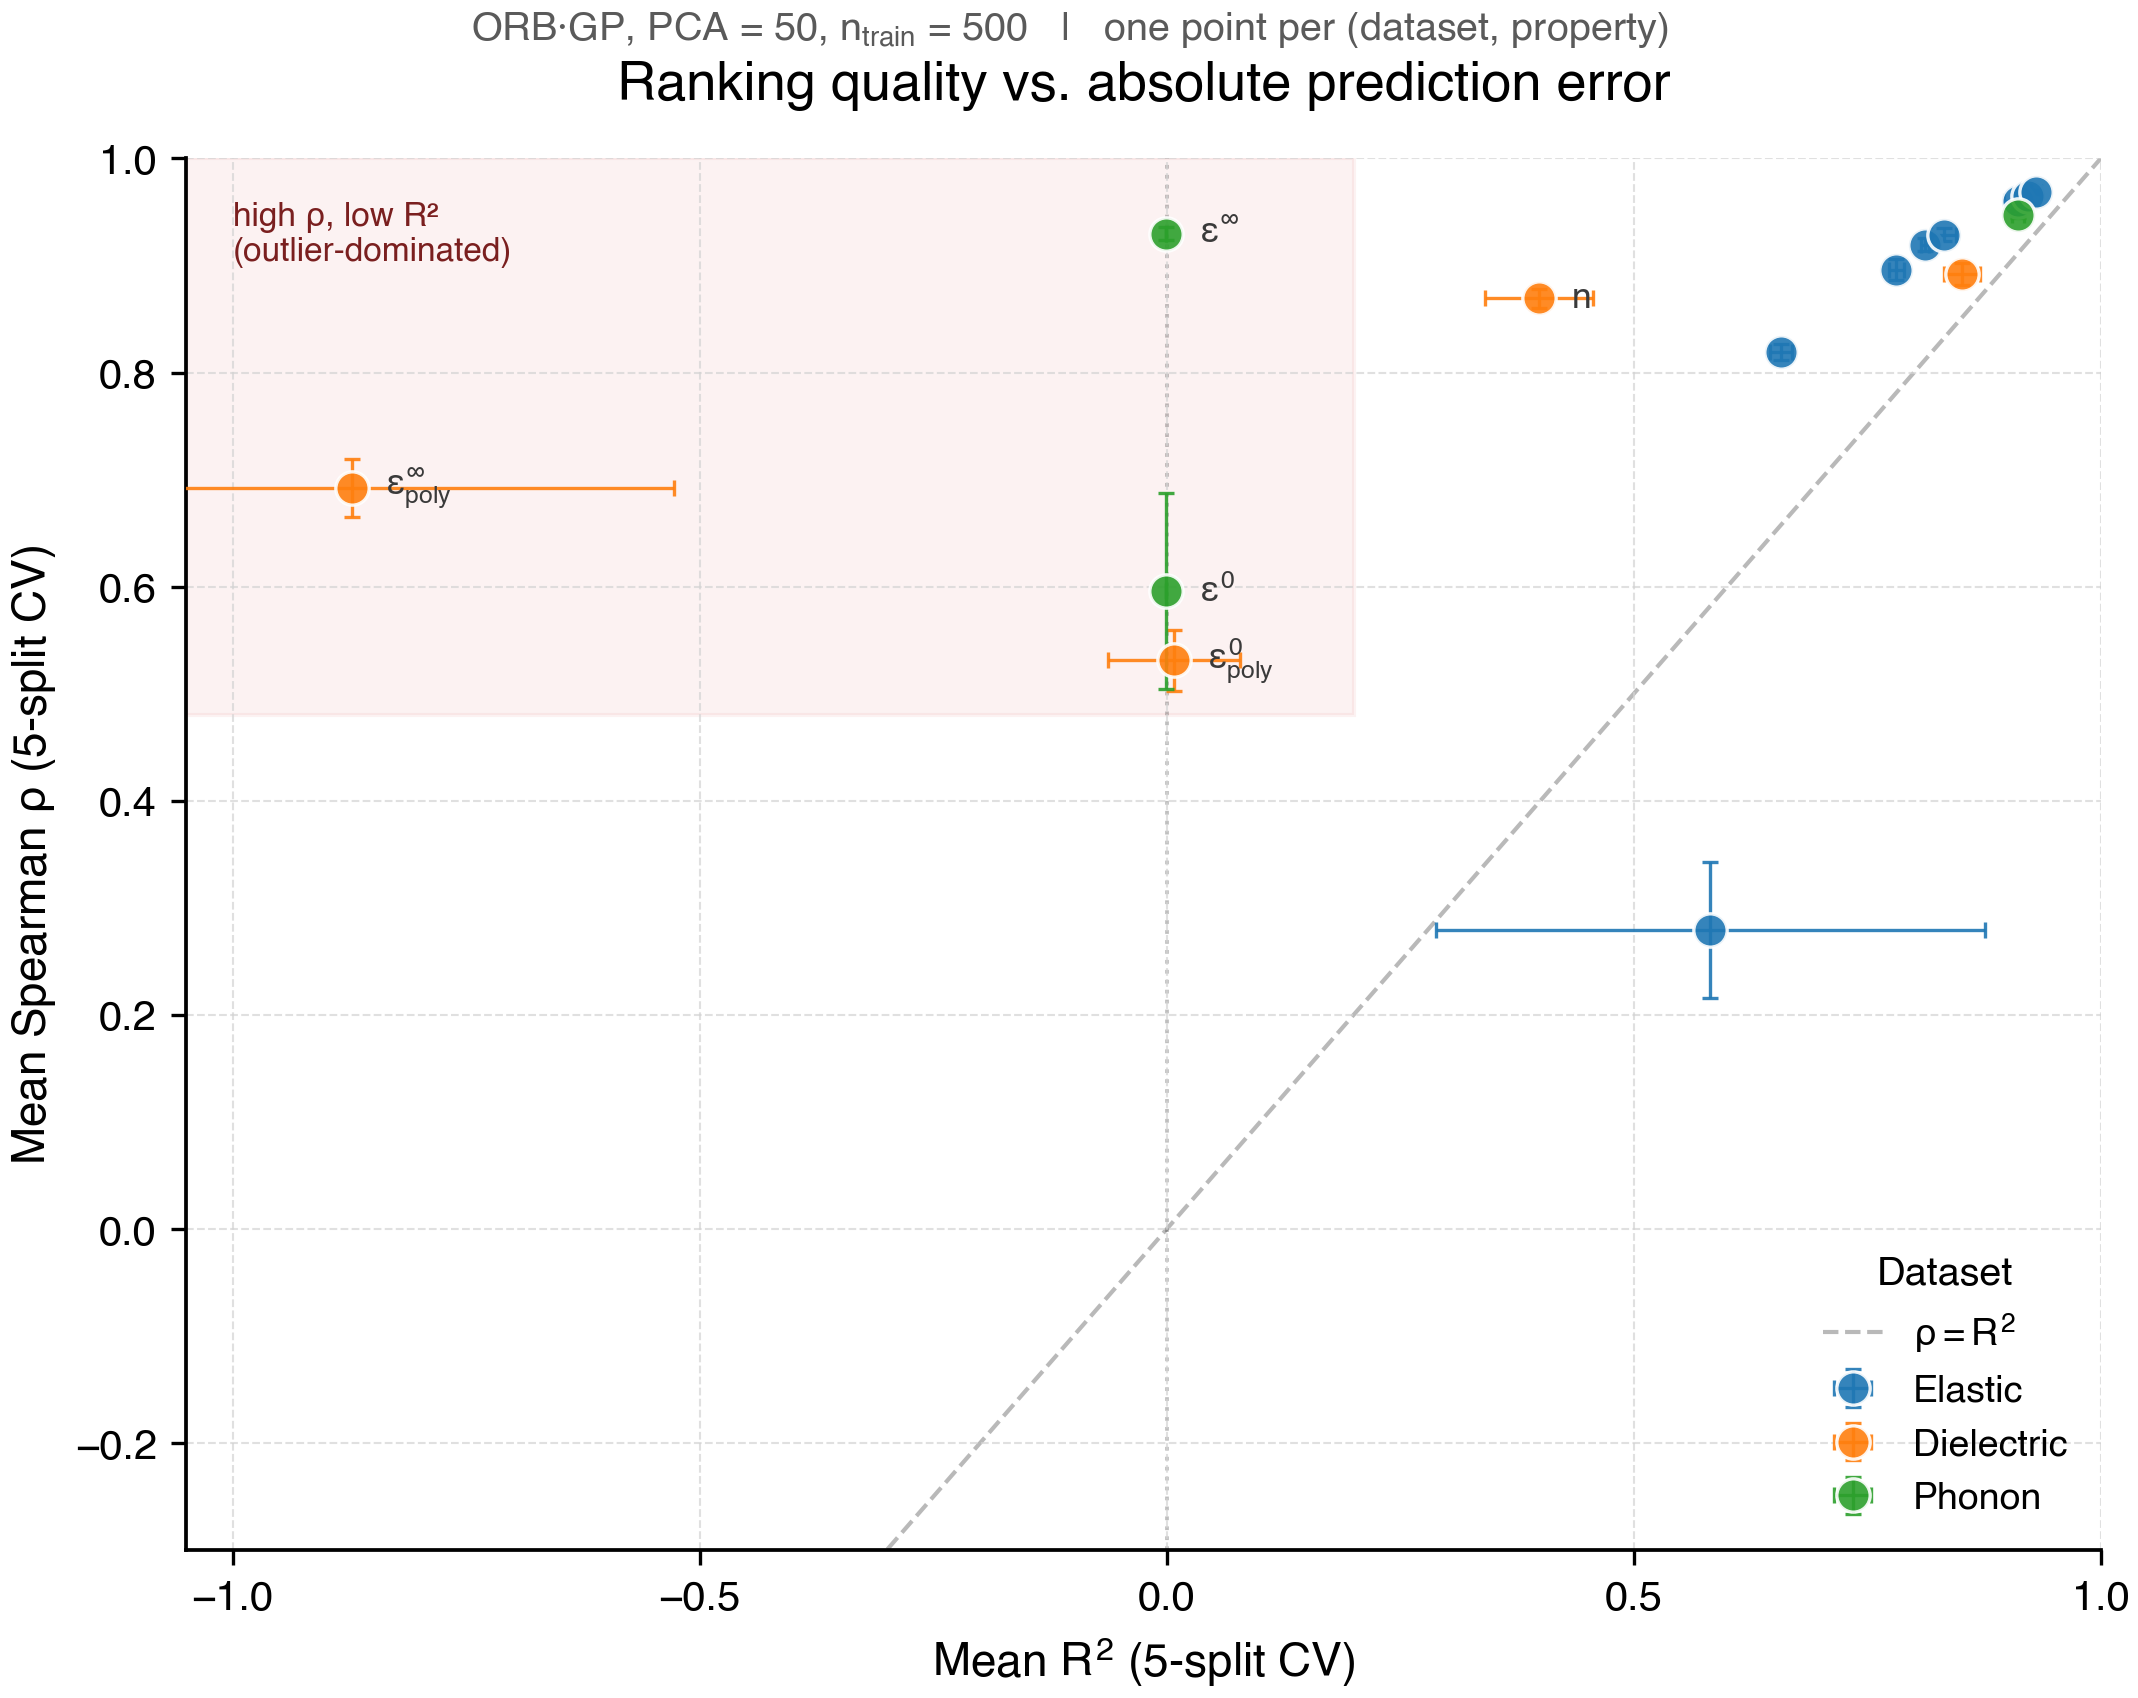
\includegraphics[width=\columnwidth]{figures/fig_metric_disagreement.png}
    \caption{Mean Spearman~$\rho$ vs.\ mean \Rtwo{} across all 16 (dataset, property) pairs under ORB\,+\,GP, PCA\,=\,50, $\ntrain = 500$, with 5-split standard-deviation bars. Points on the dashed $\rho = R^{2}$ diagonal indicate metric agreement. The shaded zone marks the regime where rank correlation remains high while \Rtwo{} collapses---driven by extreme outliers in the property distribution. Properties with $R^{2} < 0.3$ are labelled.}
    \label{fig:metric_disagreement}
\end{figure}

\FloatBarrier
Figure~\ref{fig:parity_examples} shows the best-predicted property in each dataset under the same setting (split~1).
All three sit tightly on the diagonal with calibrated uncertainty bands.
We do not show parity for the harder properties because their absolute-scale outliers dominate the visual; their cross-property structure is what Figure~\ref{fig:metric_disagreement} captures.

\begin{figure*}[!htb]
    \centering
    \begin{subfigure}[t]{0.32\textwidth}
        \centering
        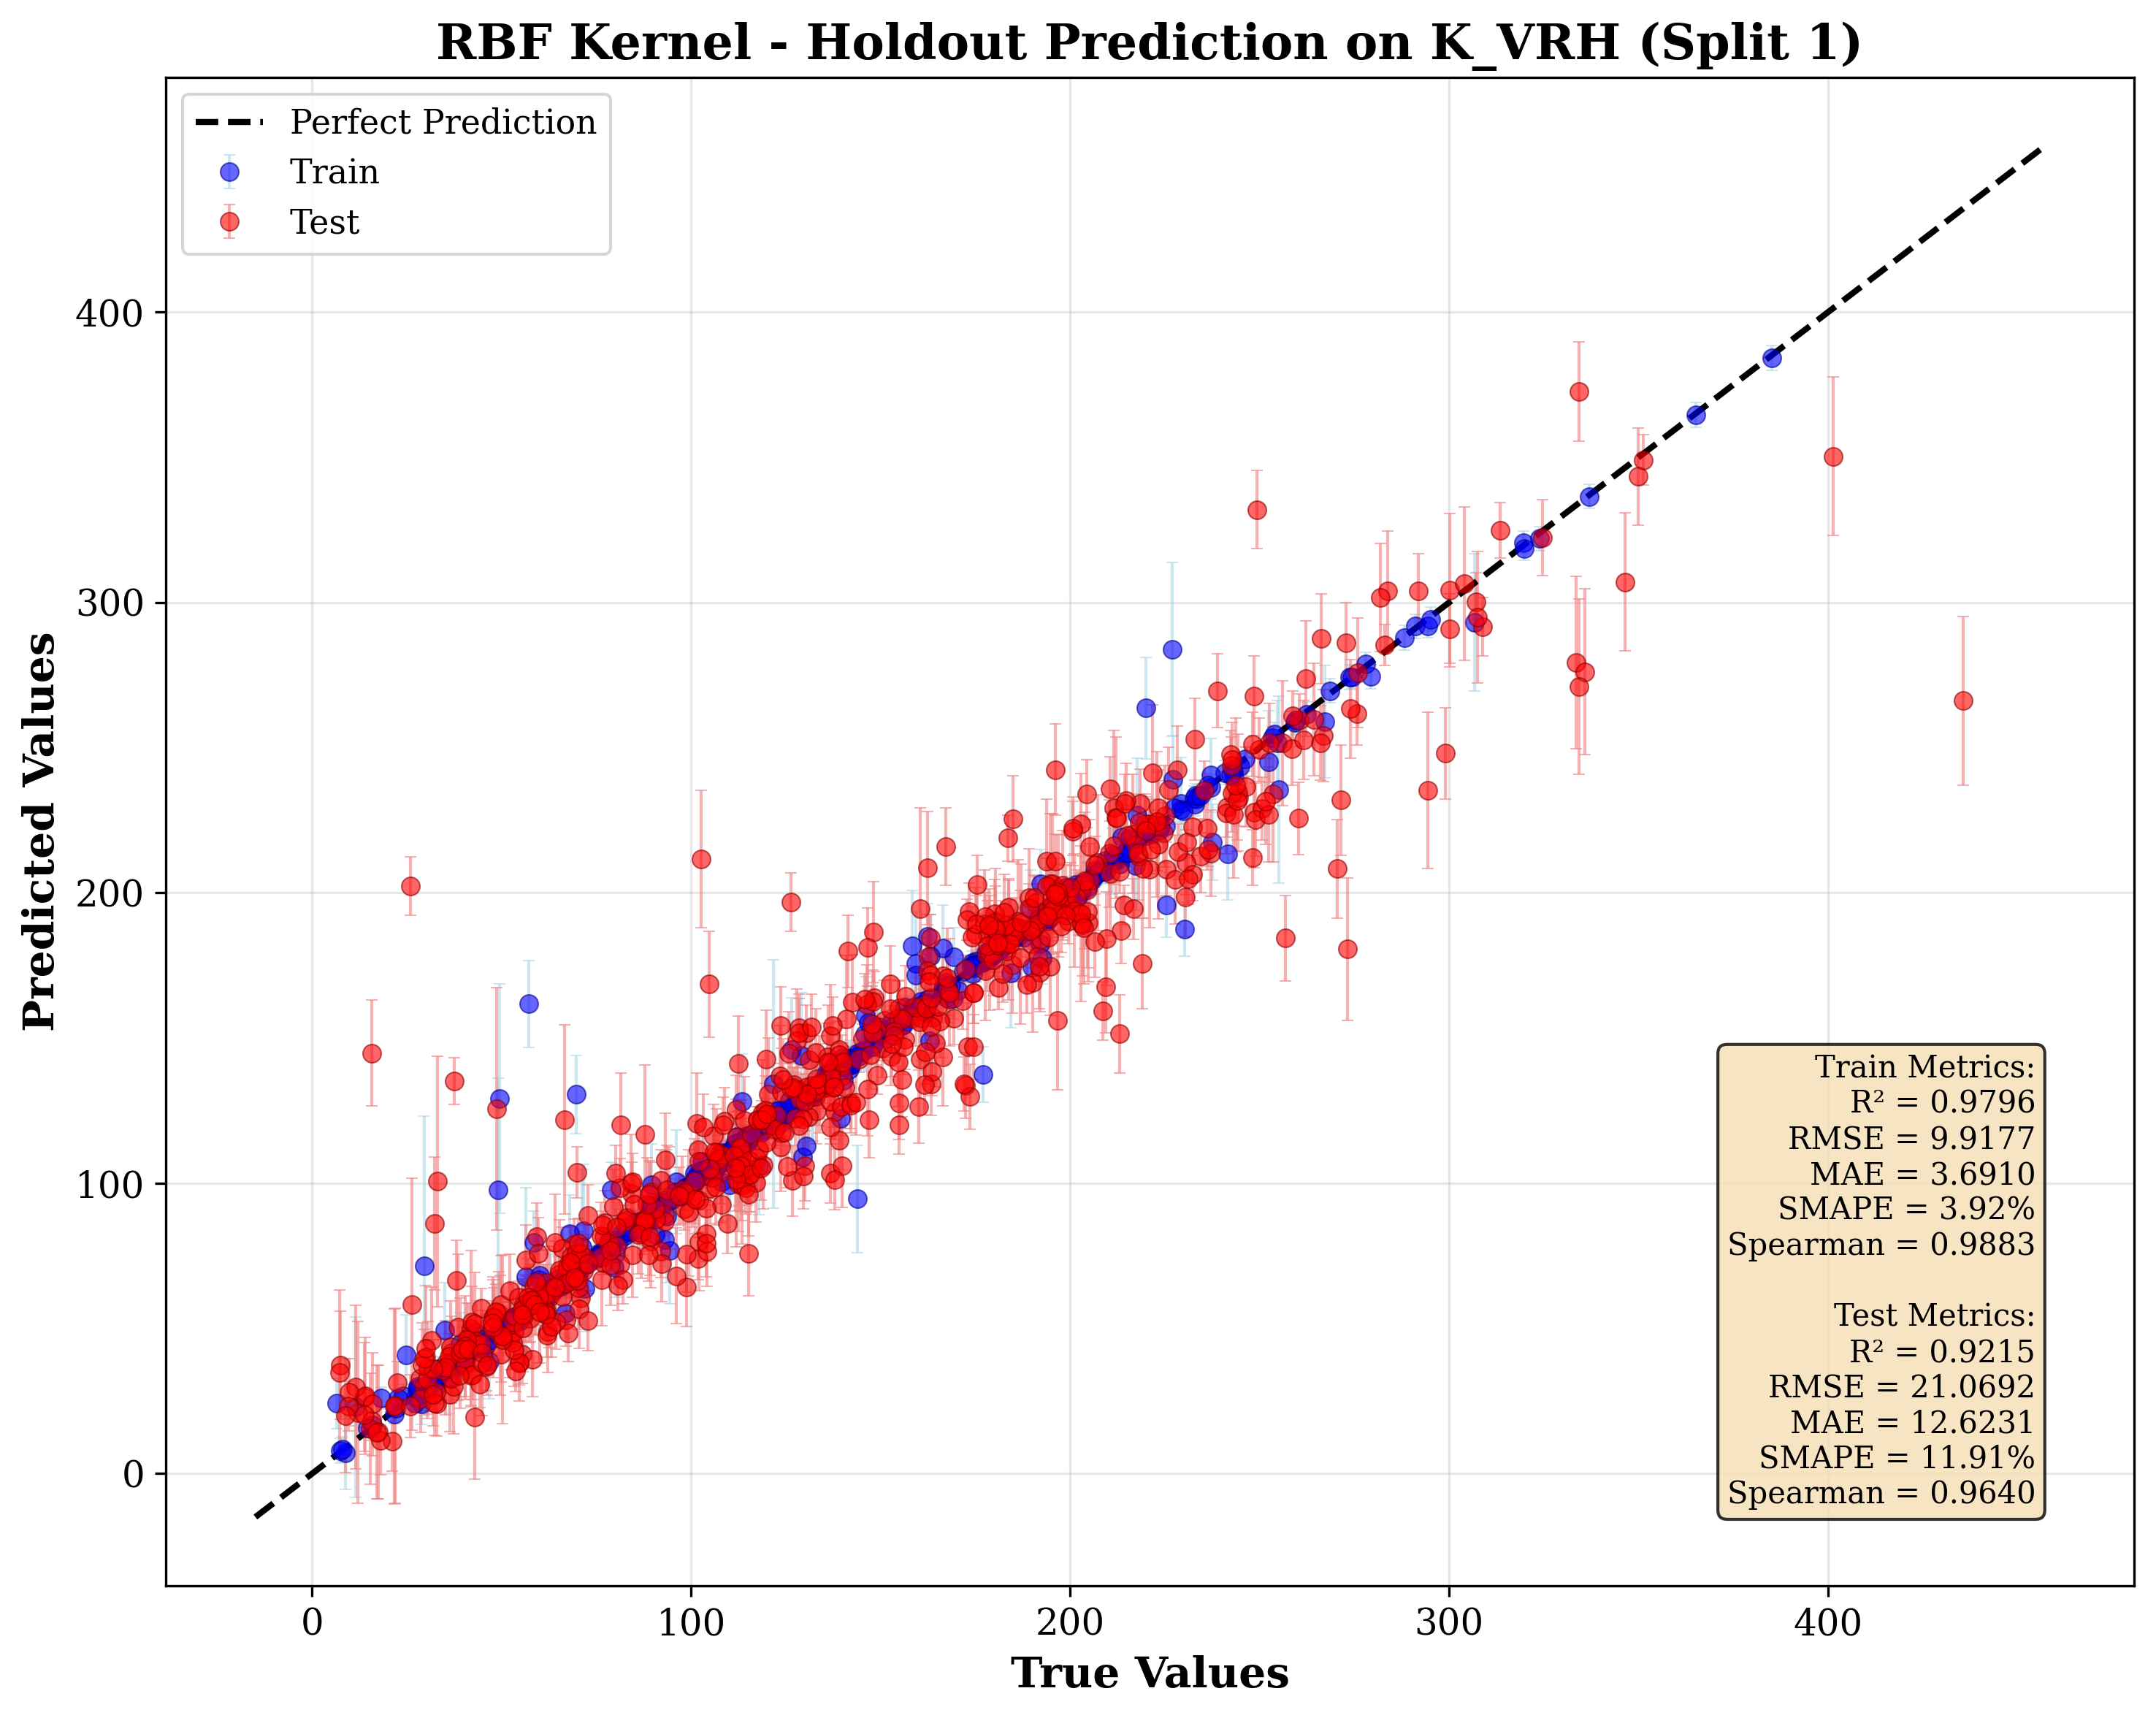
\includegraphics[width=\textwidth]{figures/fig_parity_elastic_K_VRH_orb_gp.png}
        \caption{Elastic: $K_{\text{VRH}}$ ($R^{2} = 0.922$)}
    \end{subfigure}
    \hfill
    \begin{subfigure}[t]{0.32\textwidth}
        \centering
        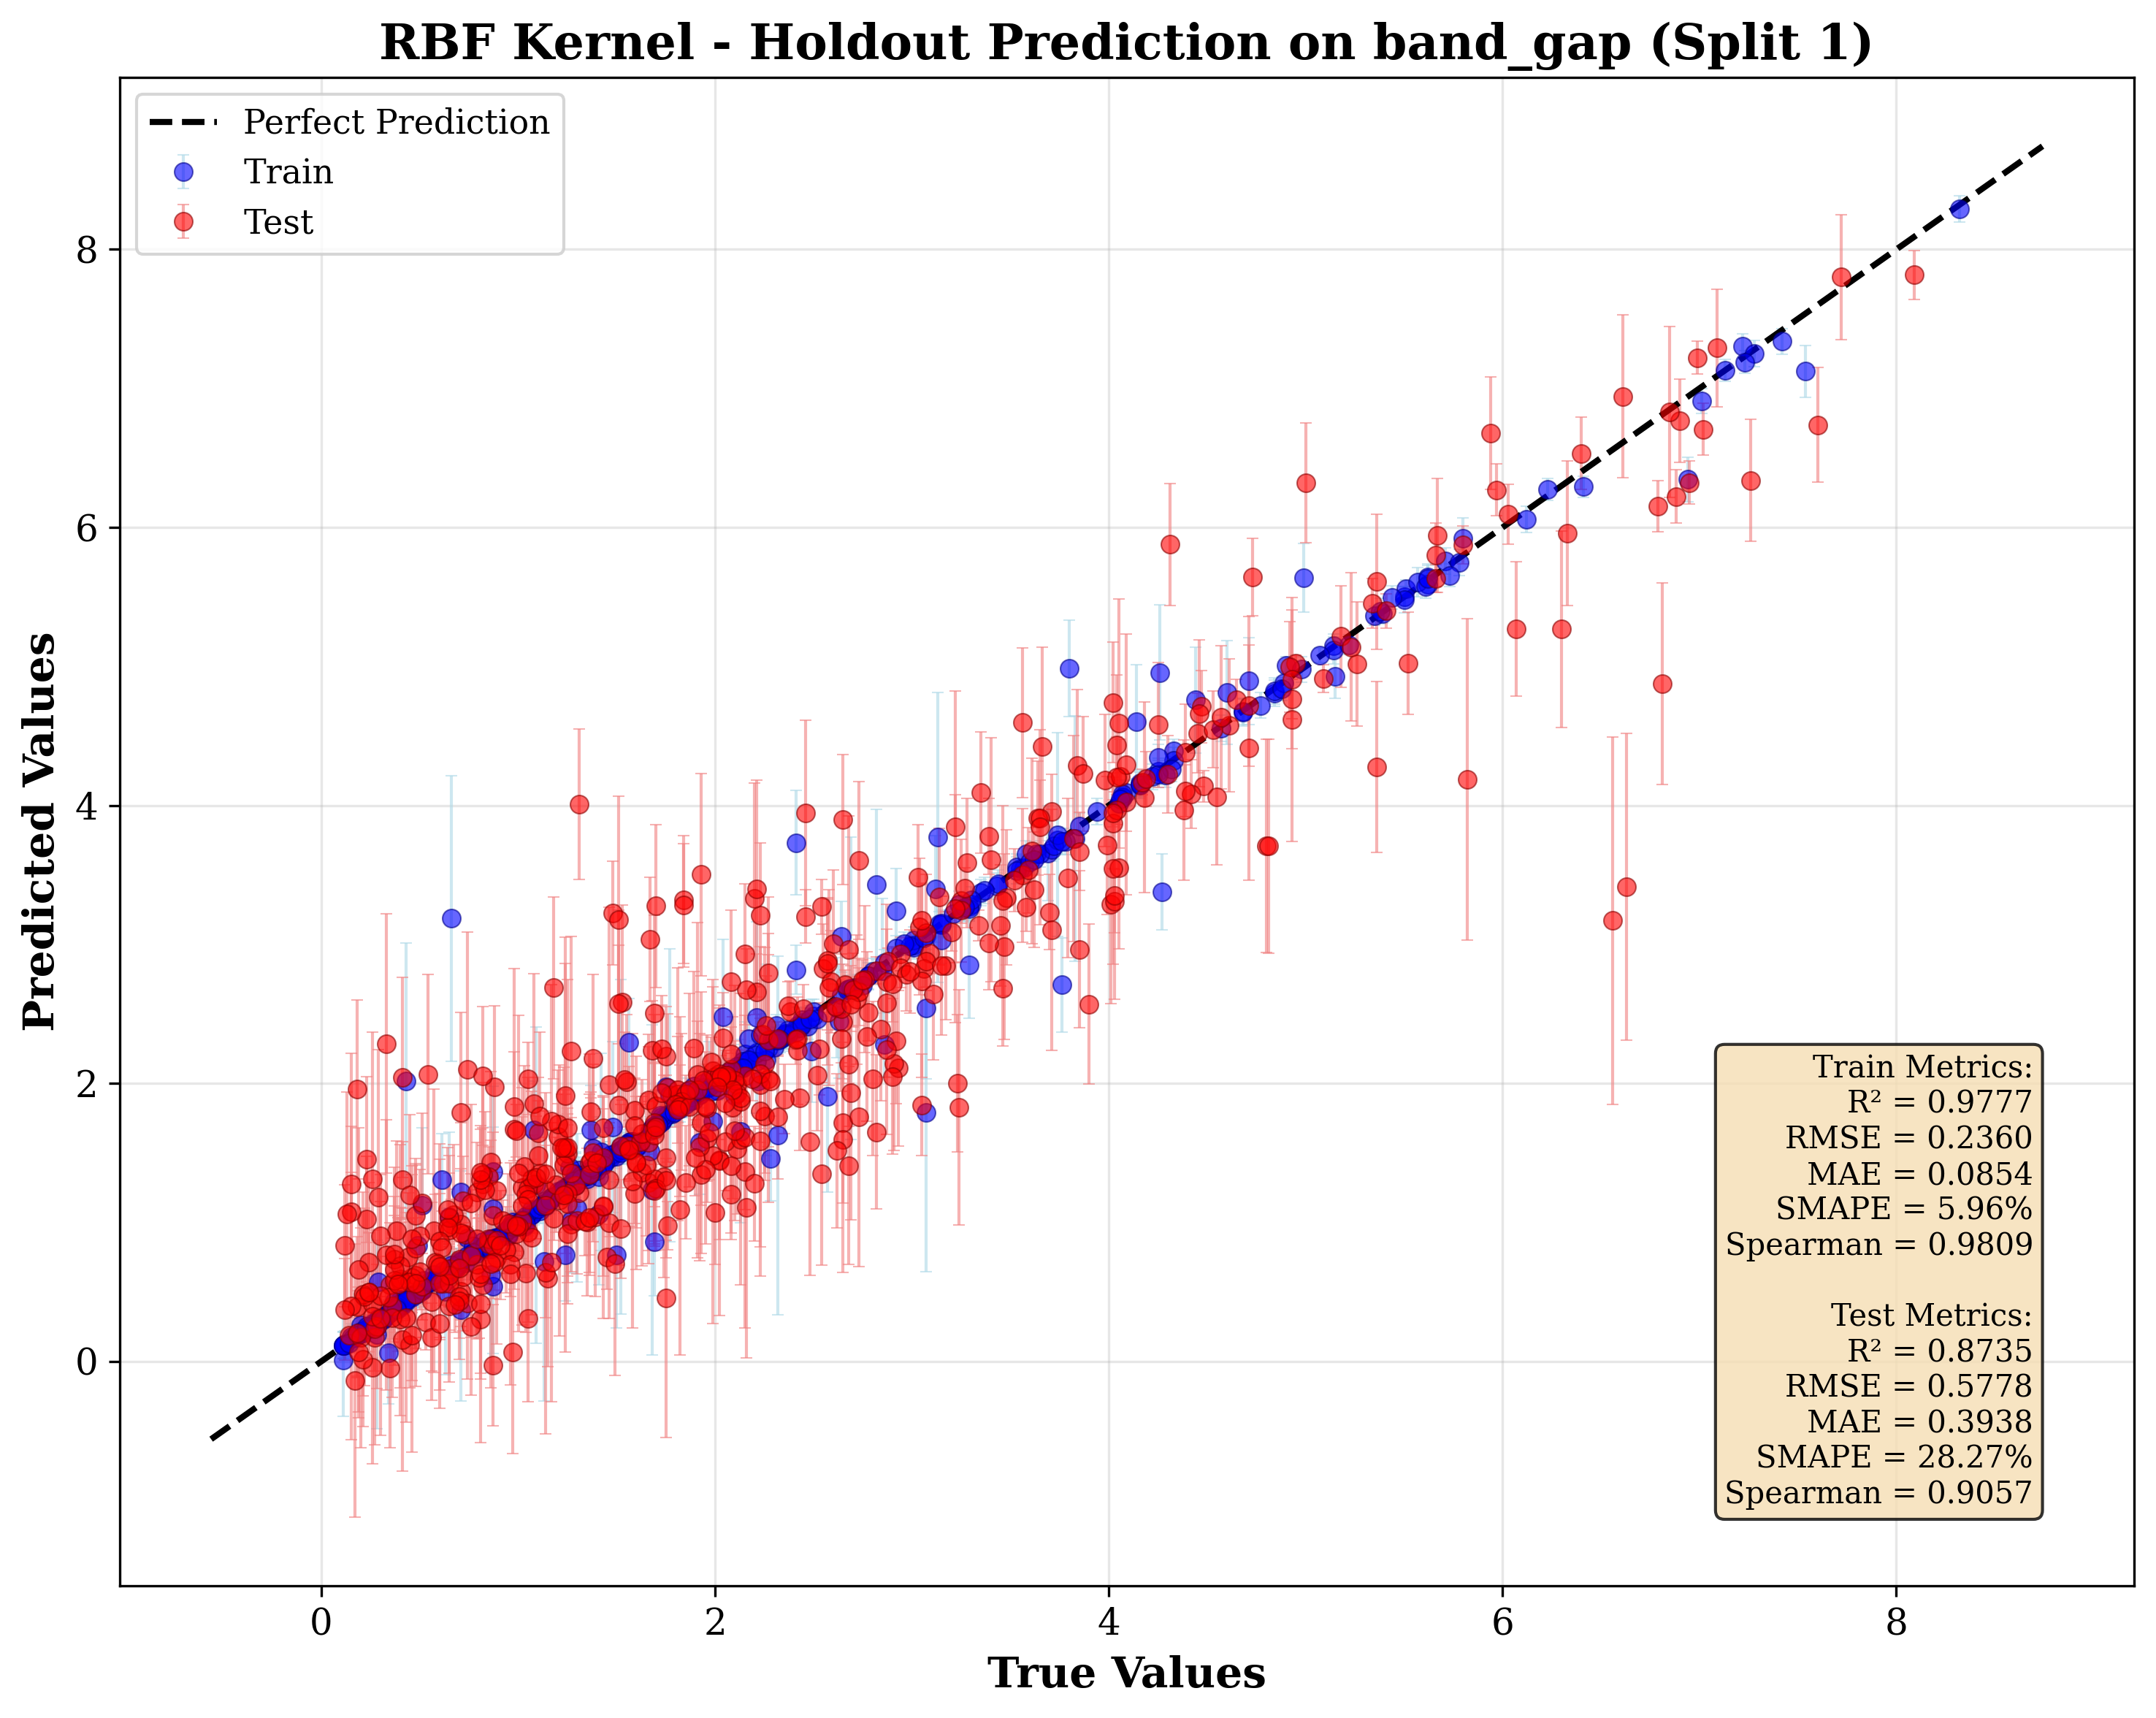
\includegraphics[width=\textwidth]{figures/fig_parity_dielectric_band_gap_orb_gp.png}
        \caption{Dielectric: band gap ($R^{2} = 0.852$)}
    \end{subfigure}
    \hfill
    \begin{subfigure}[t]{0.32\textwidth}
        \centering
        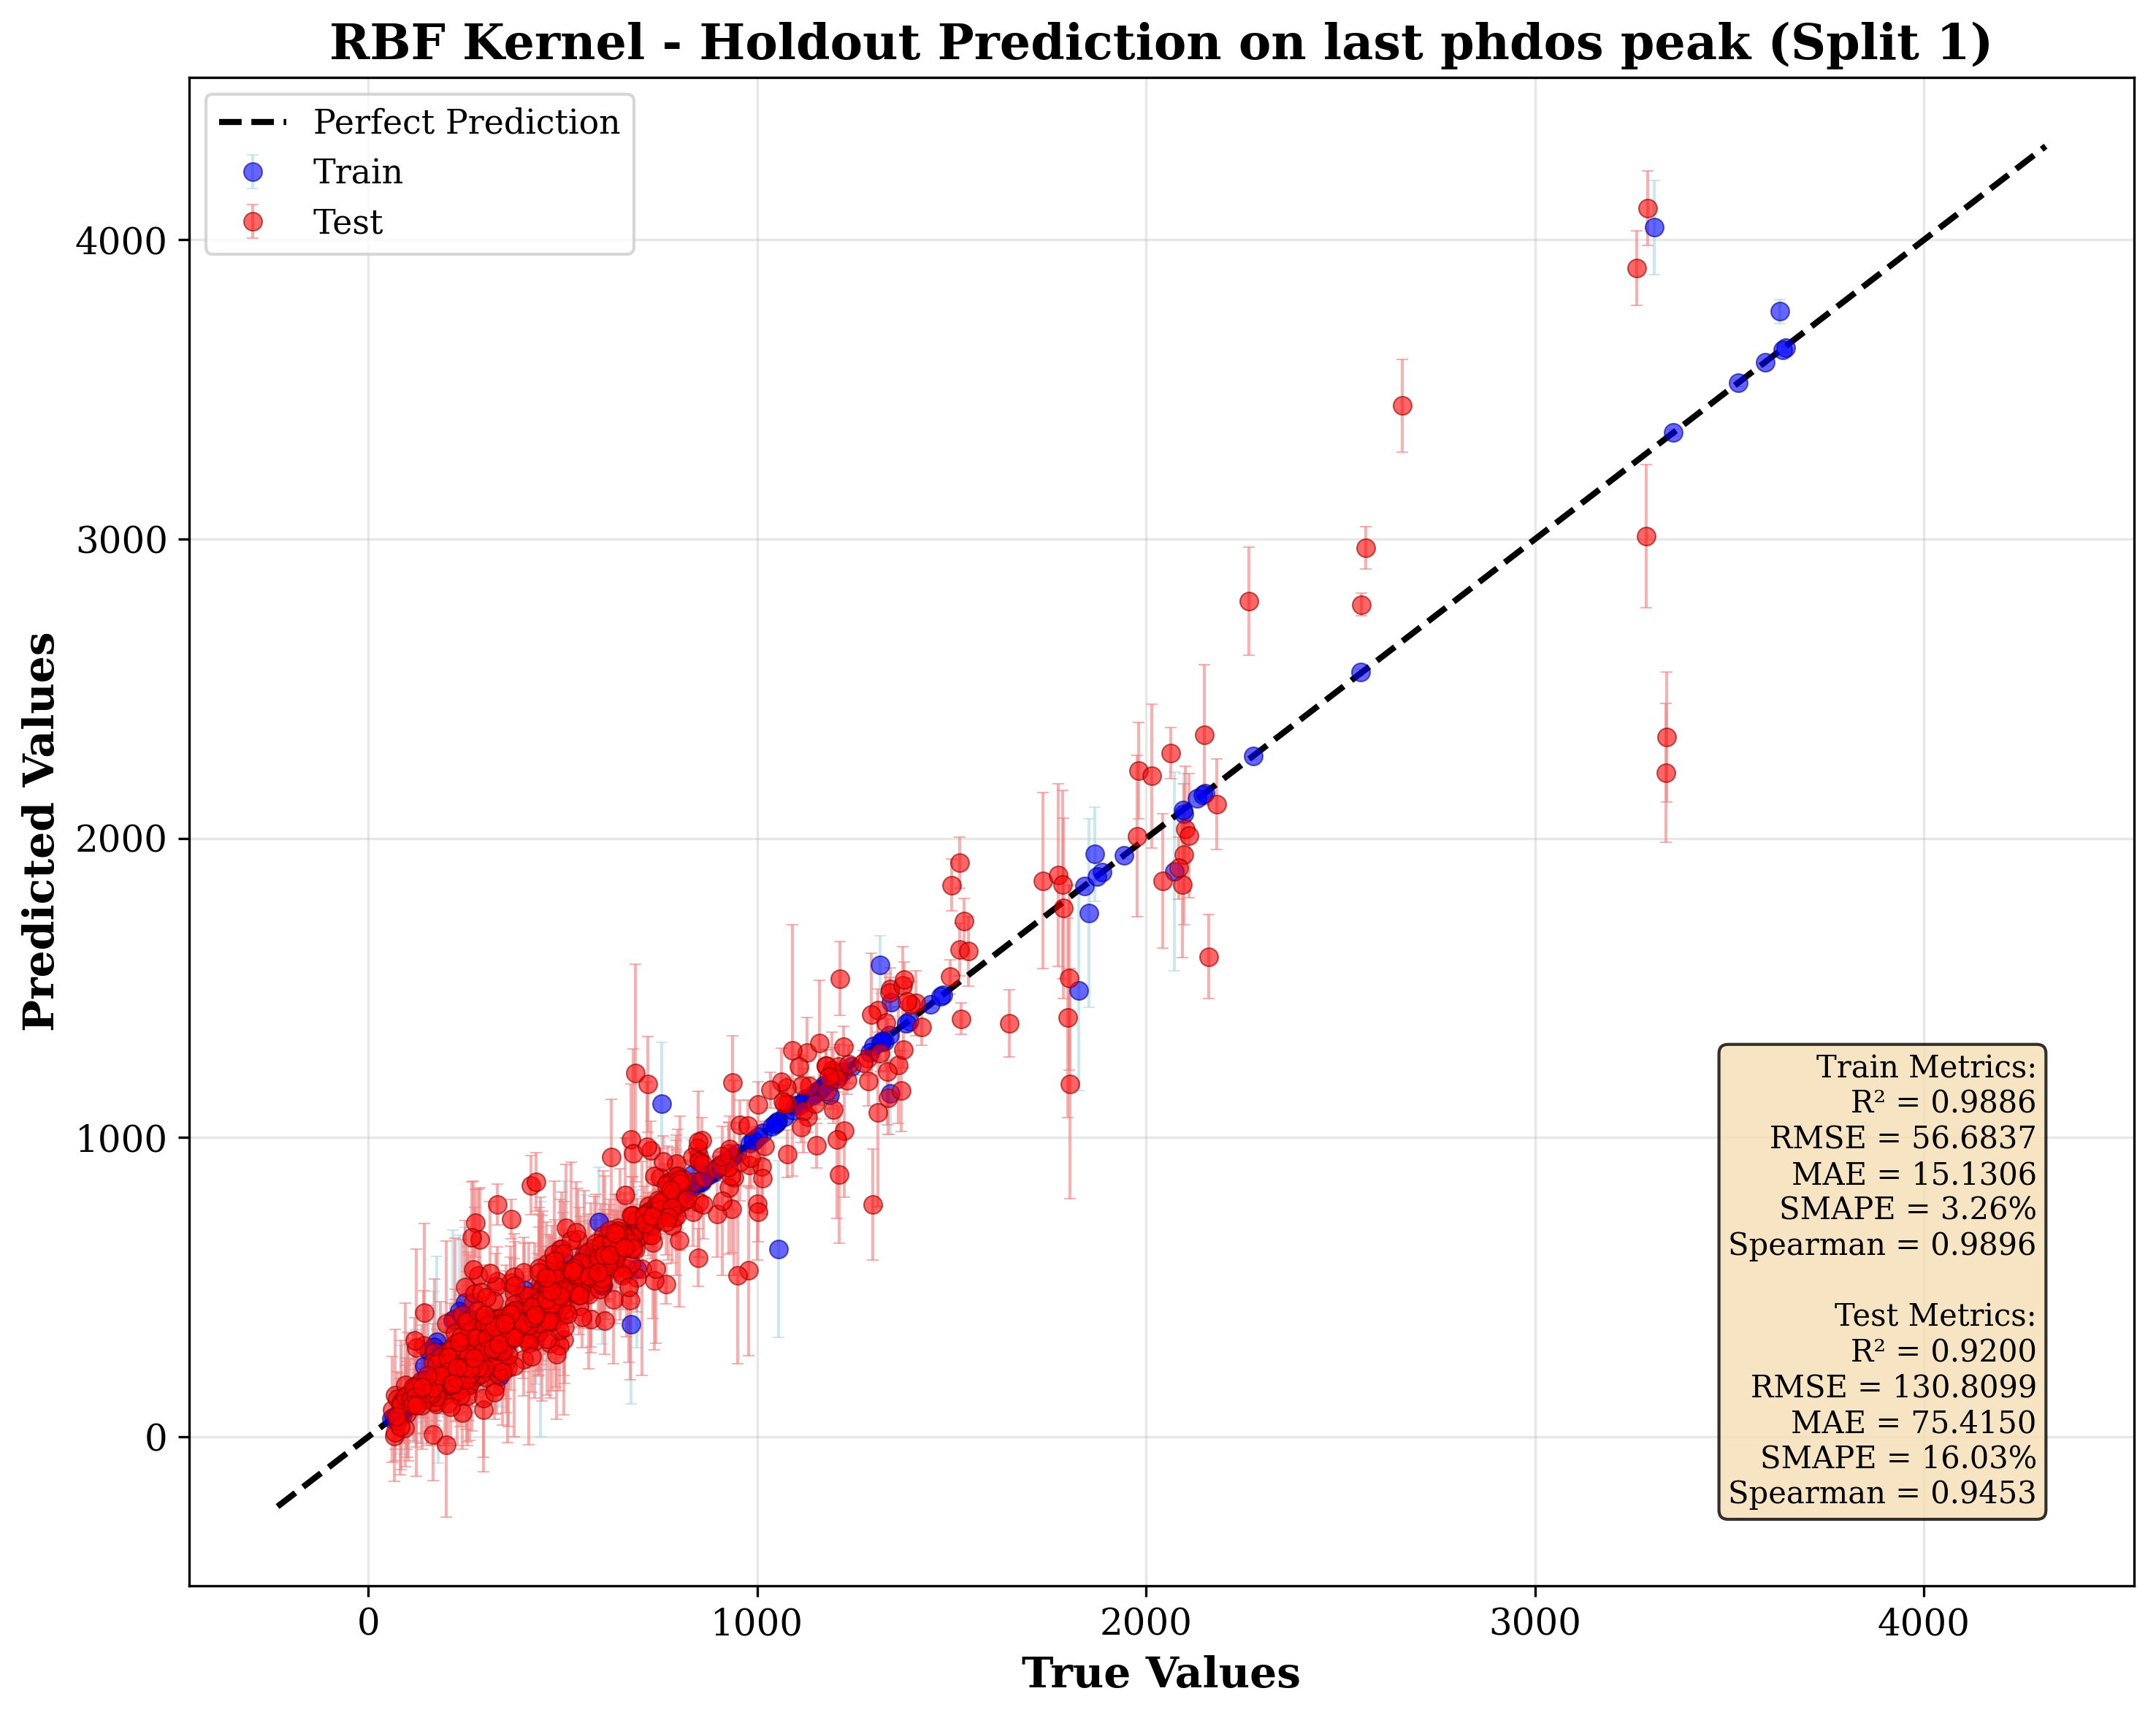
\includegraphics[width=\textwidth]{figures/fig_parity_phonon_phdos_peak_orb_gp.png}
        \caption{Phonon: phdos peak ($R^{2} = 0.911$)}
    \end{subfigure}
    \caption{Representative parity plots for the best-predicted property in each of the three benchmark datasets (ORB\,+\,GP, PCA\,=\,50, $\ntrain = 500$, split~1). All three show tight clustering around the diagonal with well-calibrated uncertainty bands.}
    \label{fig:parity_examples}
\end{figure*}

\FloatBarrier
\subsection{Cross-Dataset Synthesis}
\label{sec:cross_dataset}

Table~\ref{tab:cross_dataset} summarises the key findings across all three datasets, revealing both universal patterns and dataset-specific insights.

\begin{table*}[!htb]
    \centering
    \caption{Cross-dataset comparison at $\ntrain = 500$. For each dataset, we report the best configuration and its averaged metrics, together with the easiest and hardest properties.}
    \label{tab:cross_dataset}
    \footnotesize
    \begin{tabular}{@{}llccll@{}}
        \toprule
        \textbf{Dataset} & \textbf{Best Config} & \textbf{Avg.\ \Rtwo{}} & \textbf{Avg.\ $\rho$} & \textbf{Easiest Property} & \textbf{Hardest Property} \\
        \midrule
        Elastic tensor & ORB+DGP+PCA25 & 0.807 & 0.826 & $K_{\text{Voigt}}$ (0.931) & Poisson (0.658) \\
        Dielectric     & DGP+ORB+PCA10 & 0.336 & 0.778 & band\_gap (0.852) & poly\_elec ($-$0.180) \\
        Phonon dielec. & GP+ORB+PCA50  & 0.303 & 0.824 & phdos\_peak (0.911) & eps\_elec ($-$0.001) \\
        \bottomrule
    \end{tabular}
\end{table*}

Figure~\ref{fig:cross_descriptor} visualises this comparison: for each descriptor, we show the best achievable \Rtwo{} and Spearman~$\rho$ across all three datasets, with the name of the best-performing surrogate overlaid on each bar.

\begin{figure*}[!htb]
    \centering
    \begin{subfigure}[t]{0.48\textwidth}
        \centering
        
\includegraphics[width=\textwidth]{figures/fig_cross_dataset_R2_by_descriptor.png}
        \caption{Best \Rtwo{} per descriptor (label = best surrogate)}
        \label{fig:cross_desc_r2}
    \end{subfigure}
    \hfill
    \begin{subfigure}[t]{0.48\textwidth}
        \centering
        
\includegraphics[width=\textwidth]{figures/fig_cross_dataset_spearman_by_descriptor.png}
        \caption{Best Spearman~$\rho$ per descriptor (label = best surrogate)}
        \label{fig:cross_desc_spearman}
    \end{subfigure}
    \caption{Cross-dataset comparison of best achievable performance per descriptor at $\ntrain = 500$. Each bar shows the best \Rtwo{} (a) or Spearman~$\rho$ (b) across all surrogate--PCA combinations, with the winning surrogate name overlaid. ORB achieves the highest \Rtwo{} on all three datasets. Spearman correlations are consistently $>$0.7 for ORB across all datasets, confirming its utility for BO even when \Rtwo{} is low.}
    \label{fig:cross_descriptor}
\end{figure*}

Three universal patterns emerge:

\textbf{Pattern 1: ORB dominance.}
ORB is the best featuriser on every dataset, every surrogate, and nearly every individual property.
Its advantage is largest on the elastic dataset ($\Delta R^2 \approx 0.07$ over UMA/MACE) and smallest on the phonon dataset ($\Delta R^2 \approx 0.03$), but it never loses.
This consistency strongly supports ORB as the default featuriser for materials BO.

\textbf{Pattern 2: DGP fragility.}
The DGP collapses at PCA\,=\,50 on all three datasets, regardless of featuriser.
This is not a coincidence: the variational inference in the two-layer DGP involves $O(d^2)$ parameters in the hidden layer, and at PCA\,=\,50 with $\ntrain = 500$, the model is severely over-parameterised.
At PCA\,$\leq$\,25, the DGP can match or exceed the GP, but the risk of catastrophic failure makes it unreliable.

\textbf{Pattern 3: Spearman outperforms \Rtwo{}.}
Across all datasets, Spearman rank correlations are substantially higher than \Rtwo{} values.
This is most dramatic on the phonon dataset, where $\bar{R}^2 = 0.303$ but $\bar{\rho} = 0.824$.
For Bayesian optimisation, where the acquisition function depends on relative rankings, this means that even ``poorly'' fitting surrogates (by \Rtwo{}) can effectively guide the search.

Beyond these universals, we find dataset-specific insights.
On the elastic dataset, the property hierarchy (bulk modulus $>$ shear modulus $>$ anisotropy $>$ Poisson's ratio) mirrors the physical hierarchy of sensitivity to geometric vs.\ electronic structure.
On the dielectric dataset, band gap and refractive index are reasonably predicted because they correlate with bonding character, while the polycrystalline dielectric constants require many-body electronic structure information beyond geometric embeddings.
On the phonon dataset, the extreme \Rtwo{}-Spearman gap for eps\_electronic ($R^2 = -0.001$, $\rho = 0.930$) suggests that log-transforming or robust-scaling the target before training could dramatically improve \Rtwo{} without sacrificing ranking ability.

\FloatBarrier
\subsection{Closed-Loop Probe with Diffusion Backbones}
\label{sec:closed_loop_probe}

The static benchmark predicts an ORB\,+\,GP surrogate should remain useful in closed-loop Bayesian optimisation (BO) when $R^{2}$ is low but $\rho$ is high.
We tested this with three architecturally distinct pretrained diffusion priors, fine-tuned online via the policy-gradient procedure of MatInvent~\cite{chen2025matinvent}, with a Gaussian Process surrogate inserted between the SUN-filter and the property oracle.
The reinforcement-learning side of the procedure follows the lineage of DDPO~\cite{black2023ddpo} and DPOK~\cite{fan2023dpok} from the image domain, ported to crystals by MatInvent and (concurrently, for an autoregressive transformer prior) by CrystalFormer-RL~\cite{cao2025crystalformerrl}.
Existing tutorials and reviews of RL fine-tuning of diffusion models~\cite{uehara2024rldiffusion} catalogue several policy-gradient and value-based families, none of which include a Bayesian-optimisation gate at acquisition time; the recent npj Comp Mat review of generative AI for crystals~\cite{generative_review_2025} surveys the design space without devoting a section to closed-loop, online surrogate-gated refinement, although it does note one offline precedent---Qi et al.'s Latent Conservative Objective Models (LCOM)~\cite{qi2023lcom}, which trains a conservative surrogate over a CDVAE latent space to minimise formation energy.
LCOM differs from the present work in being offline (no online policy update of the generator), single-property (formation energy), and built around a CDVAE rather than a diffusion prior; we view it as a complementary precedent rather than a baseline.
The probe in this section sits in that gap.

We ran two property targets ($C_p$ and $K_{\text{VRH}}$), two policies (BASE and ACC, defined below), three backbones, and five seeds---thirty closed-loop runs in total, with a matching set for the bulk-modulus target.
The diffusion priors are not retrained from scratch; they are updated only through online REINFORCE-style rollouts.
The oracle is itself a learned surrogate (eSEN-30M-OAM~\cite{uma2025} fed into phonopy~\cite{togo2015first} for $C_p$ and a Birch--Murnaghan fit~\cite{birch1947finite} for $K_{\text{VRH}}$), and top candidates are not DFT-validated here.
With those caveats noted, the runs are large enough to examine cross-backbone behaviour, characterise the GP surrogate as the loop progresses, and report the practical effect of inserting the gate into a published RL pipeline.

\subsubsection{Pipeline and Setup}
\label{sec:cl_pipeline}

The three backbones are MatterGen~\cite{zeni2025mattergen} (\texttt{mg}), CrystalFlow~\cite{luo2025crystalflow} (\texttt{cf}), and ADiT~\cite{joshi2025adit} (\texttt{adit}).
Each runs under two policies.
BASE follows the published MatInvent recipe~\cite{chen2025matinvent} verbatim: policy-gradient updates with reward-weighted KL regularisation against the pretrained prior ($\sigma = 0.025$), an experience-replay buffer (size 100, sample size 10, reward cutoff 0.1), and a diversity filter on the long-term memory (tolerance 3, buffer 6).
ACC differs from BASE only in the property calculator: between the SUN filter and the oracle it inserts a Gaussian Process surrogate over ORB\,+\,PCA50 features, scores SUN-survivors by the acquisition rule (Expected Improvement plus a Determinantal Point Process diversity term), and dispatches only the top $K = 4$ to the oracle each cycle; the remaining candidates receive NaN reward, so they do not contribute to the policy-gradient update.
Every other RL hyperparameter (KL coefficient, replay buffer, diversity filter, finetune epochs, batch size $\sim 16$ candidates per cycle) is byte-identical between BASE and ACC.
Each run lasts 20 cycles, and every candidate passes the Stable+Unique+Novel (SUN) screen before any oracle or surrogate call.

\begin{figure}[H]
    \centering
    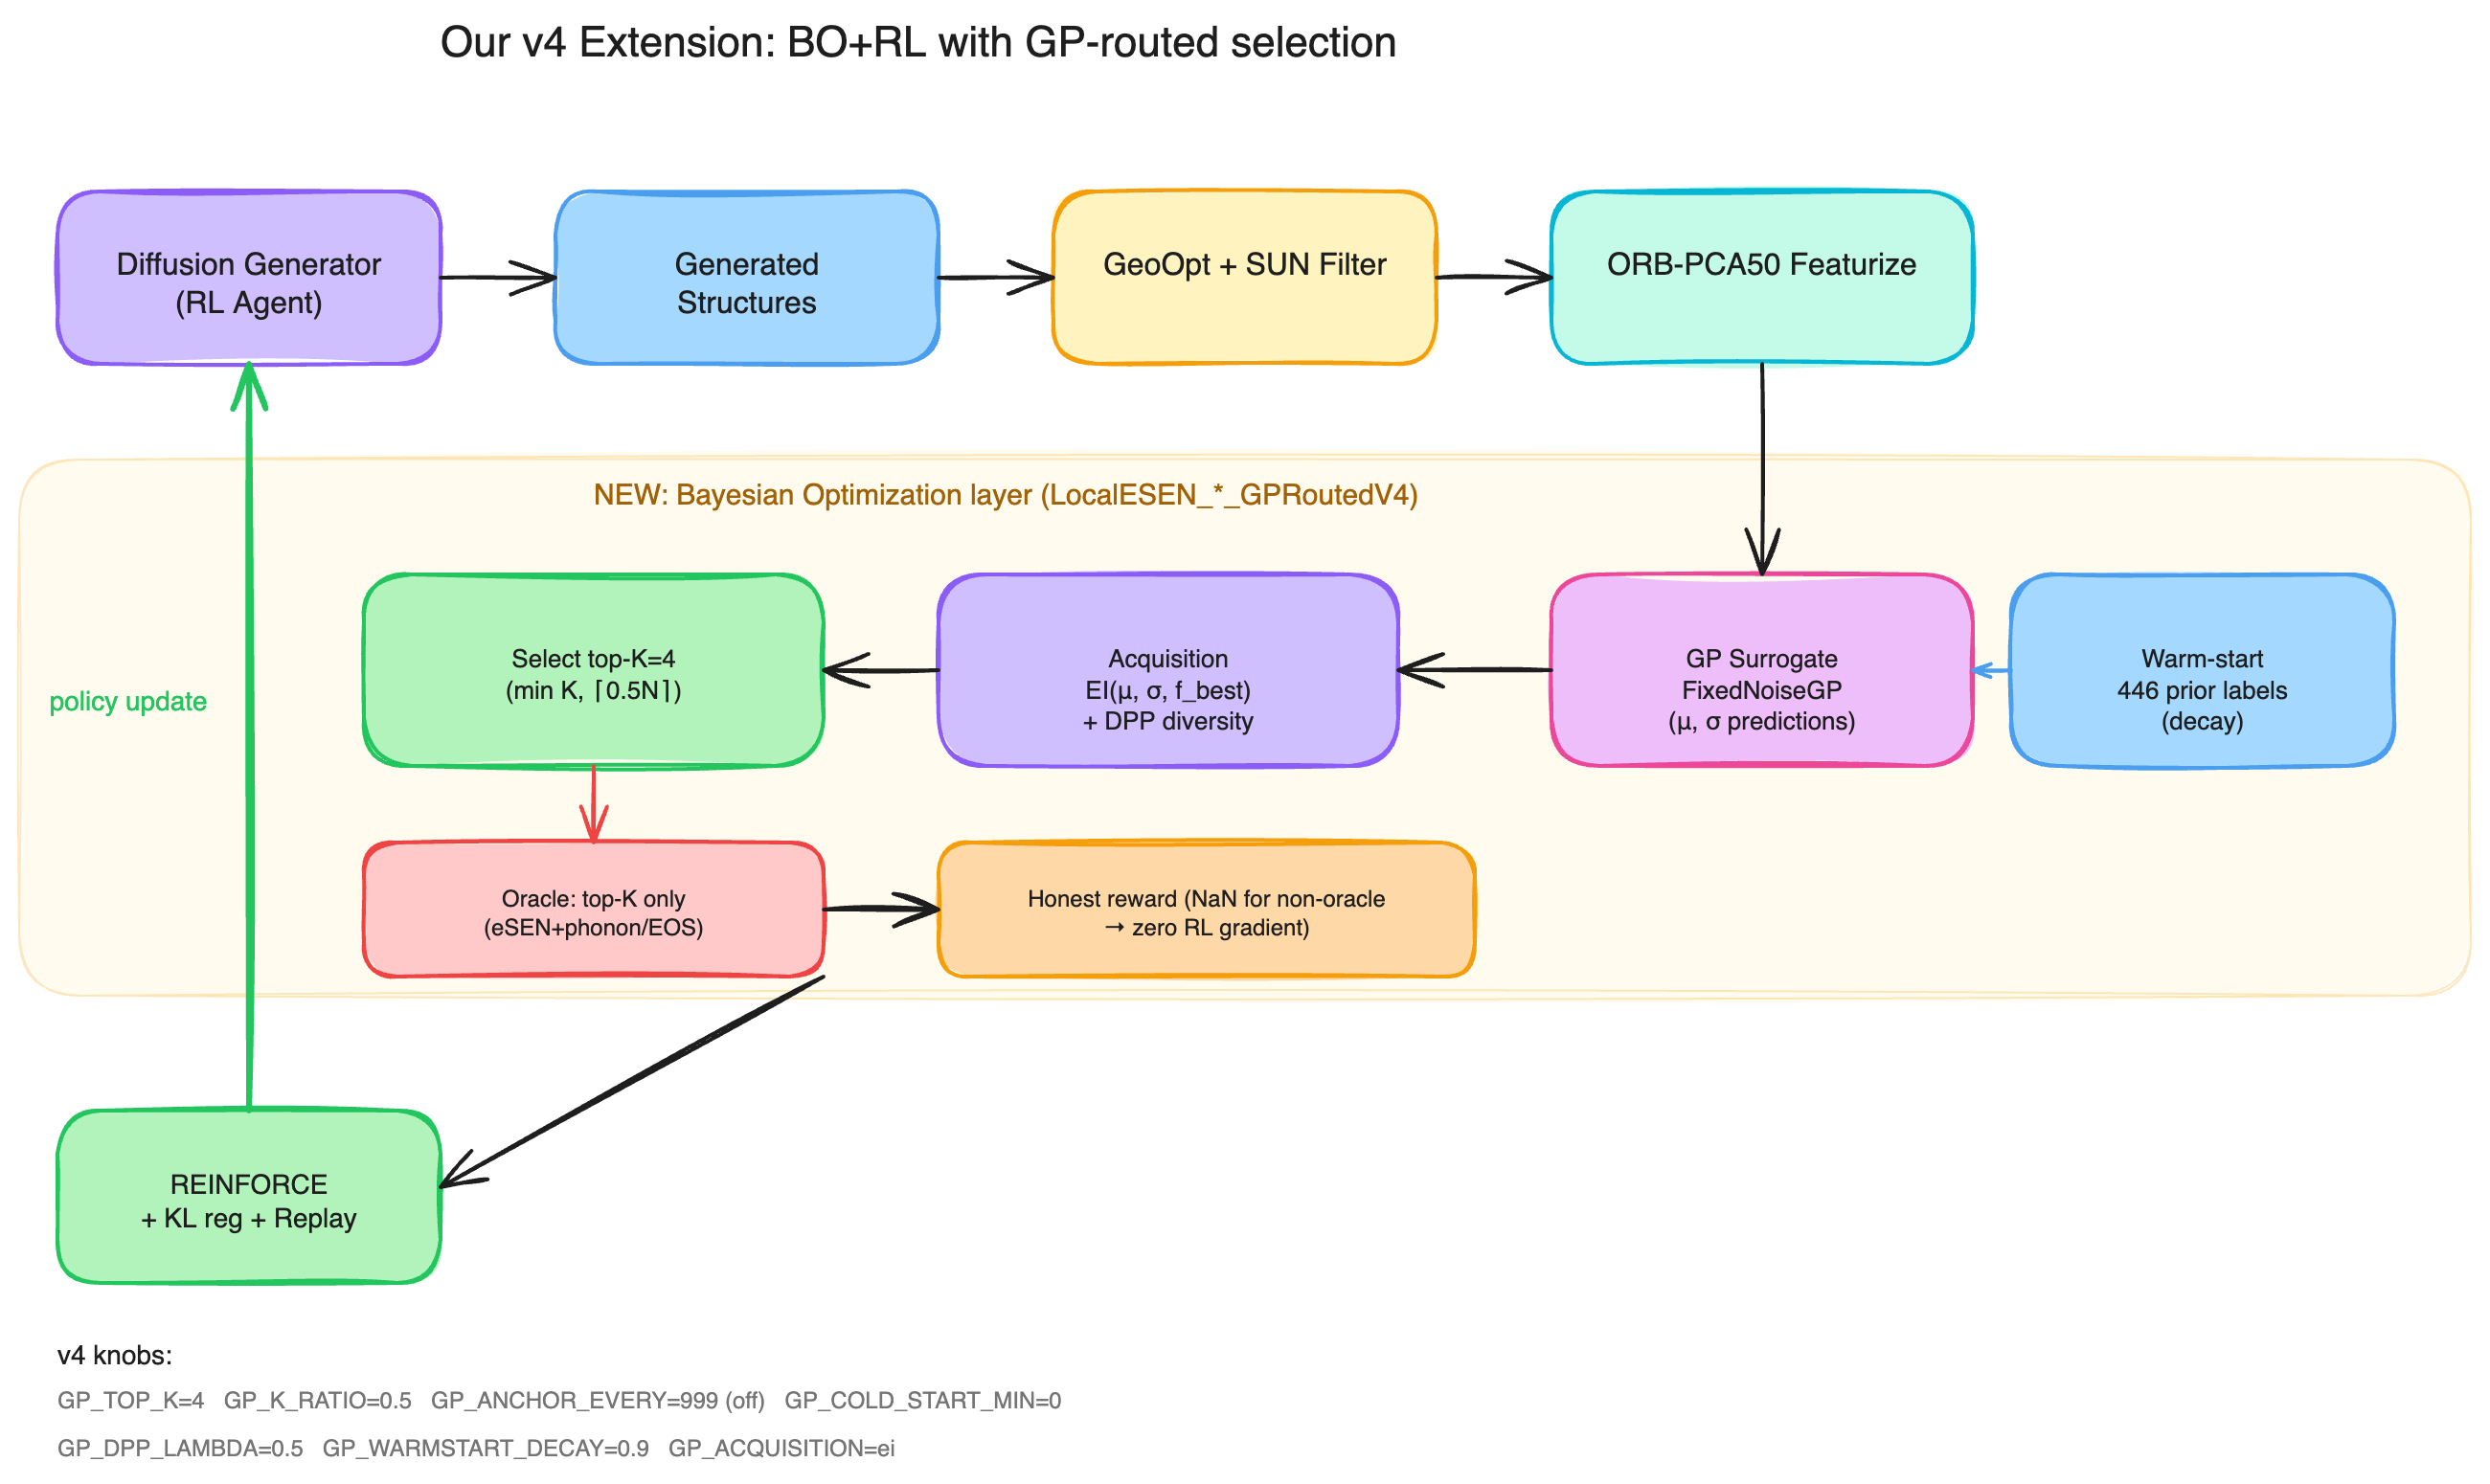
\includegraphics[width=\columnwidth]{figures/fig_closed_loop_pipeline.png}
    \caption{The closed-loop pipeline. The diffusion generator proposes structures; geometry optimisation and a SUN filter remove unstable, duplicate, or non-novel candidates; ORB\,+\,PCA50 featurises the survivors; the GP scores them; an acquisition rule (EI plus a DPP diversity term) selects the top $K=4$; only those reach the oracle (eSEN+phonon for $C_p$, EOS fit for $K_{\text{VRH}}$); REINFORCE then updates the diffusion policy. Non-oracle candidates receive NaN rewards and contribute zero RL gradient, so the surrogate's choice of which $K$ to call is the only training signal.}
    \label{fig:closed_loop_pipeline}
\end{figure}

\FloatBarrier
\subsubsection{Discovery Curves Across Backbones}
\label{sec:cl_curves}

Figure~\ref{fig:closed_loop_curves} tracks the running best property value over the 20 cycles, broken out by backbone and policy; per-seed running-bests are forward-filled to the full cycle horizon before averaging so that the cross-seed mean is itself non-decreasing.
For $C_p$, ACC reaches 1.0--1.2~J/g/K---approaching but short of the 1.5~J/g/K reference---in all three backbones, and exceeds BASE consistently in MatterGen, ADiT, and (more modestly) CrystalFlow.
For $K_{\text{VRH}}$, MatterGen and ADiT plateau near 310~GPa under ACC; the single best structure (375~GPa) is an MoN polymorph in space group $P\,\bar{6}m2$ (\#187) found by ADiT/ACC at seed 7.
CrystalFlow shows the largest between-seed spread of the three backbones for both targets, so its mean comparison is the noisiest of the panel, but the ACC mean still sits above the BASE mean throughout.
The qualitative pattern is consistent with the static-benchmark prediction in Section~\ref{sec:spearman_r2}: a high-$\rho$, low-\Rtwo{} surrogate suffices to drive acquisition without breaking the underlying RL update.
Trajectories at cycle 20 are also consistent with the published MatInvent runs at the equivalent loop count---Fig.~2c of \cite{chen2025matinvent} (10-seed mean) shows a heat-capacity mean of roughly 0.7--0.9~J/g/K at loop 20 in their MatterGen-based setup, within the seed-level error bands of our 5-seed BASE run.

\begin{figure*}[!htb]
    \centering
    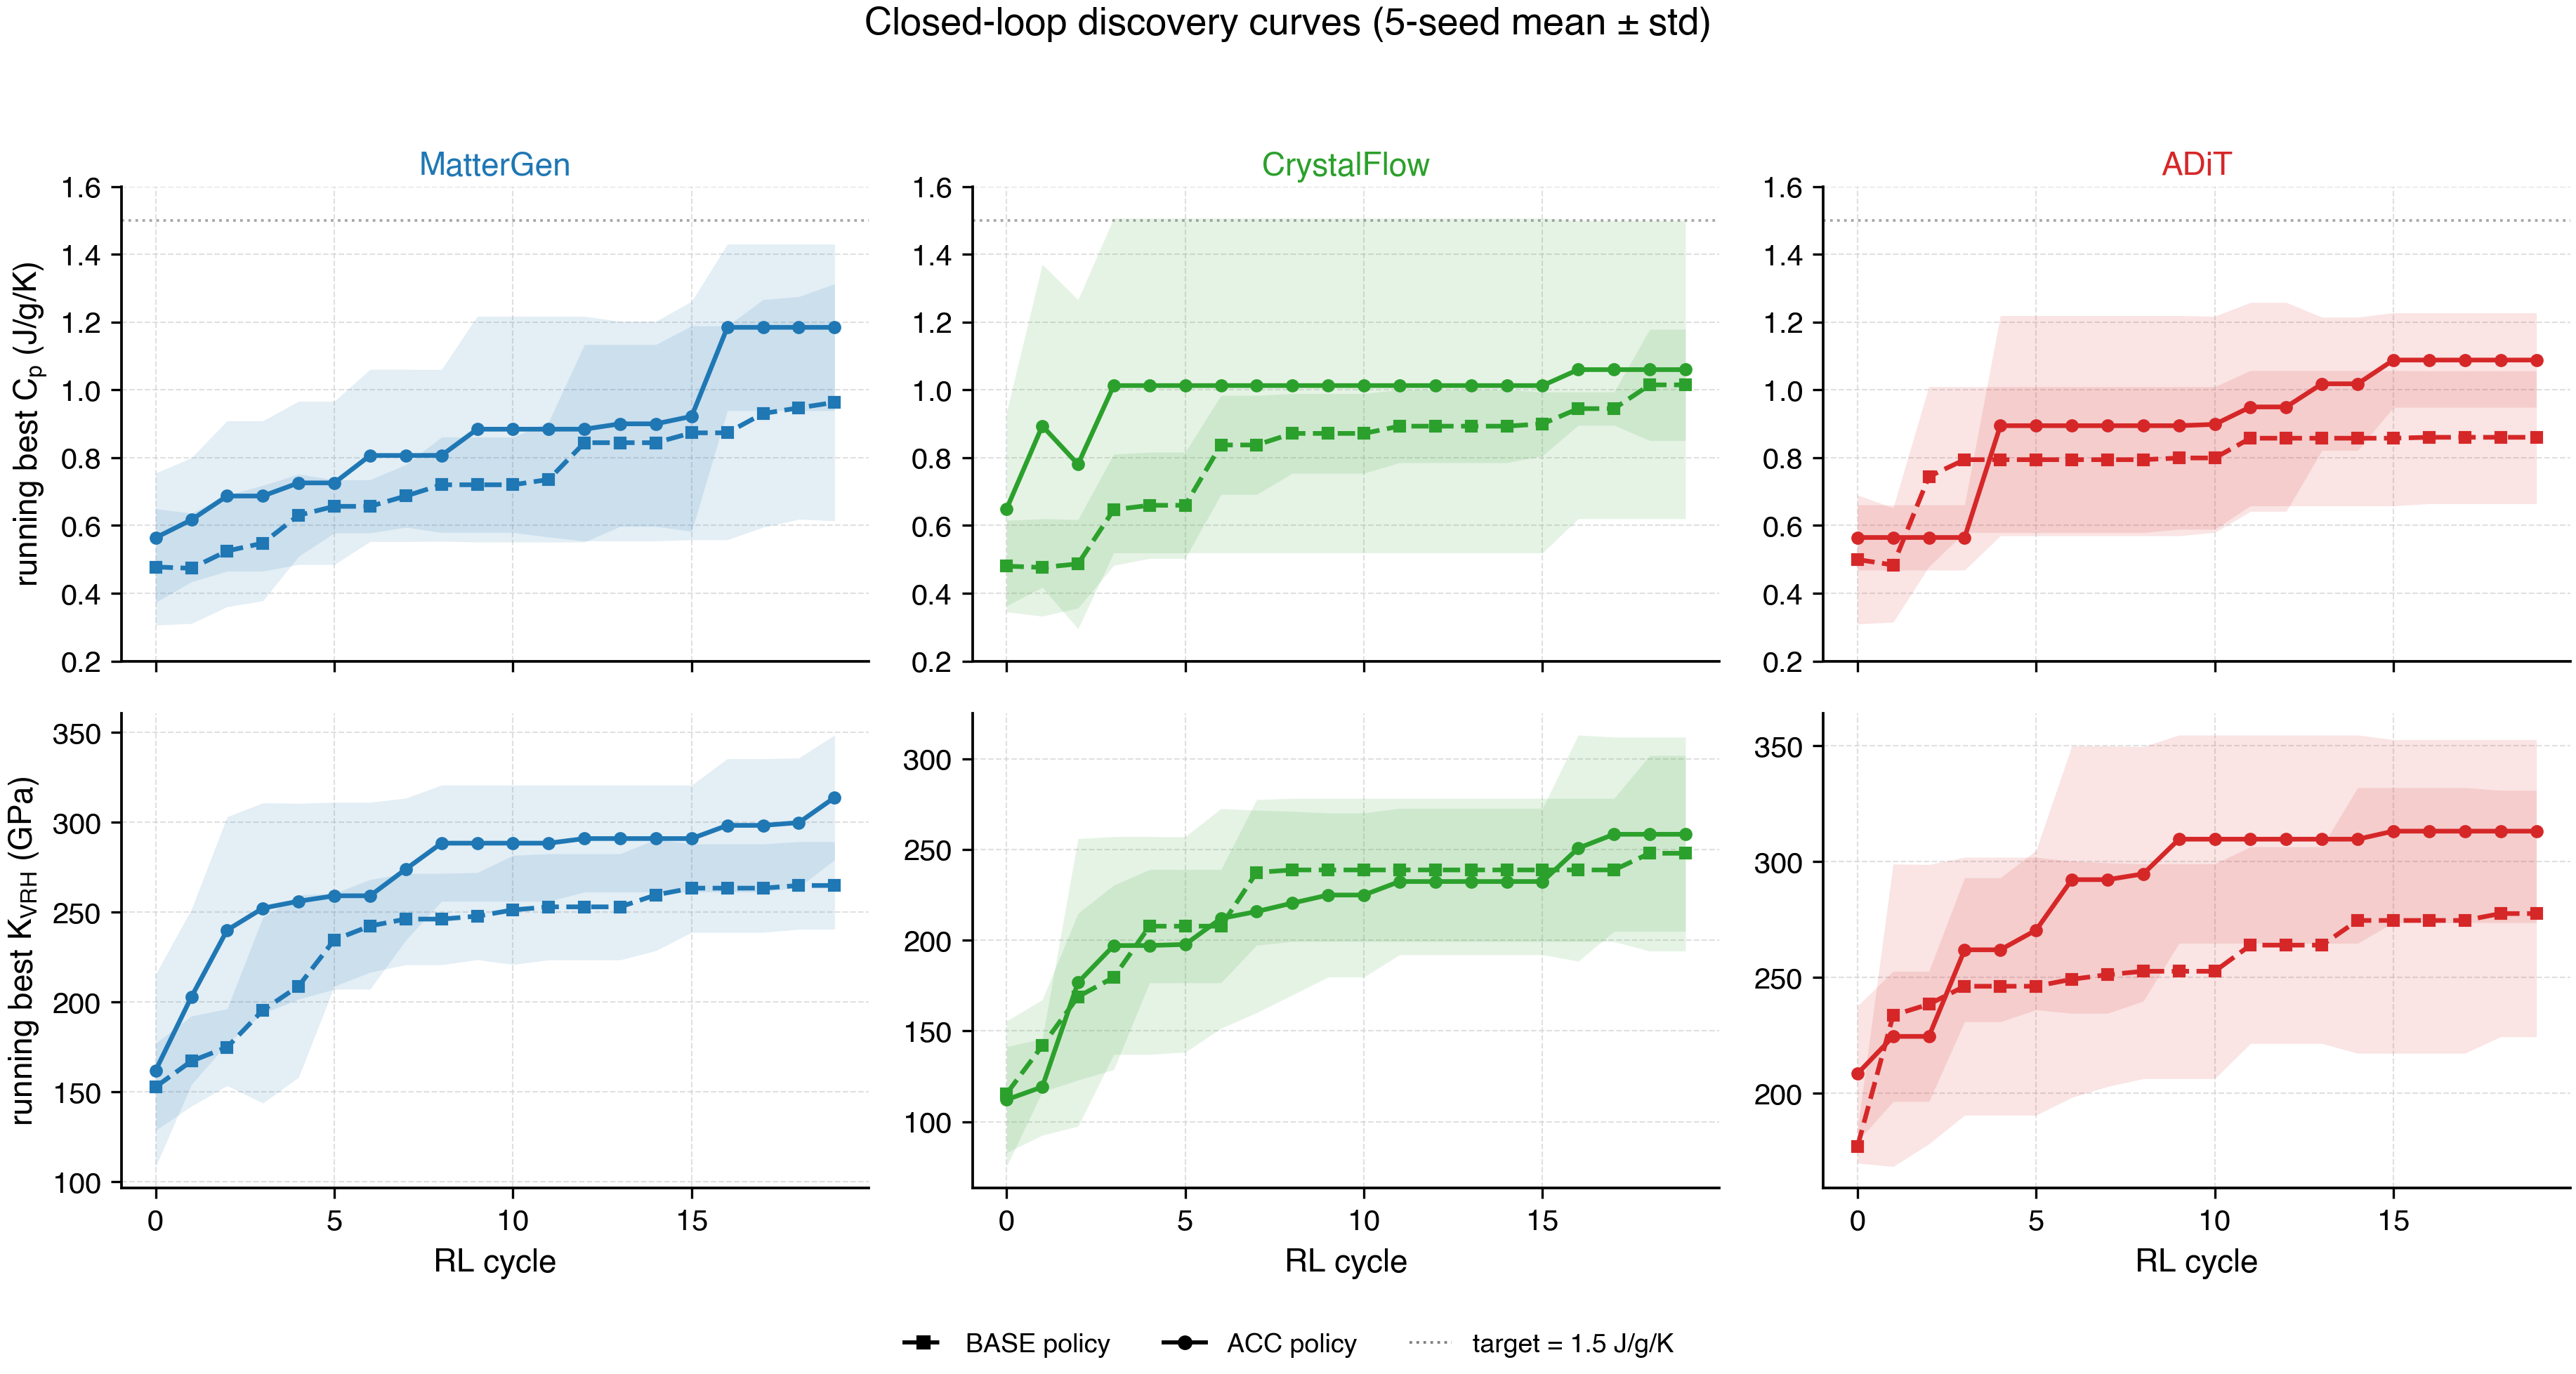
\includegraphics[width=\textwidth]{figures/fig_bogen_curves.png}
    \caption{Running best property value over 20 RL cycles, 5-seed mean $\pm$ std. Top row: $C_p$ (target $\to$ 1.5~J/g/K, dotted line). Bottom row: $K_{\text{VRH}}$ (max). Solid lines and circles: GP-gated BO (ACC); dashed lines and squares: vanilla REINFORCE (BASE). MatterGen and ADiT show a clean ACC-over-BASE lift on both targets; CrystalFlow's seed variance is too large to call either policy a winner.}
    \label{fig:closed_loop_curves}
\end{figure*}

\FloatBarrier
\subsubsection{Surrogate Quality Across Cycles}
\label{sec:cl_surrogate}

Figure~\ref{fig:closed_loop_surrogate} plots the GP CV5 RMSE per cycle, ACC runs only.
This metric is 5-fold cross-validation on the GP's accumulated training set---the oracled candidates from the warm-start plus all top-$K$ acquisitions up to the current cycle (16 points at cycle~0, growing by 4 per cycle to 92 by cycle 19).
It measures how well the GP fits its own oracled labels under leave-one-fold-out resampling; it does \emph{not} measure error on the next batch of fresh diffusion proposals, which is the quantity the gate actually uses $\mu$ to score.
On $C_p$ the CV5 RMSE sits at 0.075--0.090 (normalised property scale) and is statistically flat across cycles---mean RMSE in cycles 0--5 differs from cycles 15--19 by less than one between-seed standard deviation.
$K_{\text{VRH}}$ shows the same pattern at the 21--26~GPa level, with a mild downward trend in MatterGen and CrystalFlow.
The fair reading is that the GP remains internally consistent as the training set grows---the loop does not break self-consistency---which is a necessary but not sufficient condition for surrogate-gated BO health.
A held-out RMSE on the diffusion proposals before they reach the gate is not in our current logs; this is the metric we would need to claim true generalisation, and we flag its absence as a limitation in Section~\ref{sec:cl_caveats}.

\begin{figure*}[!htb]
    \centering
    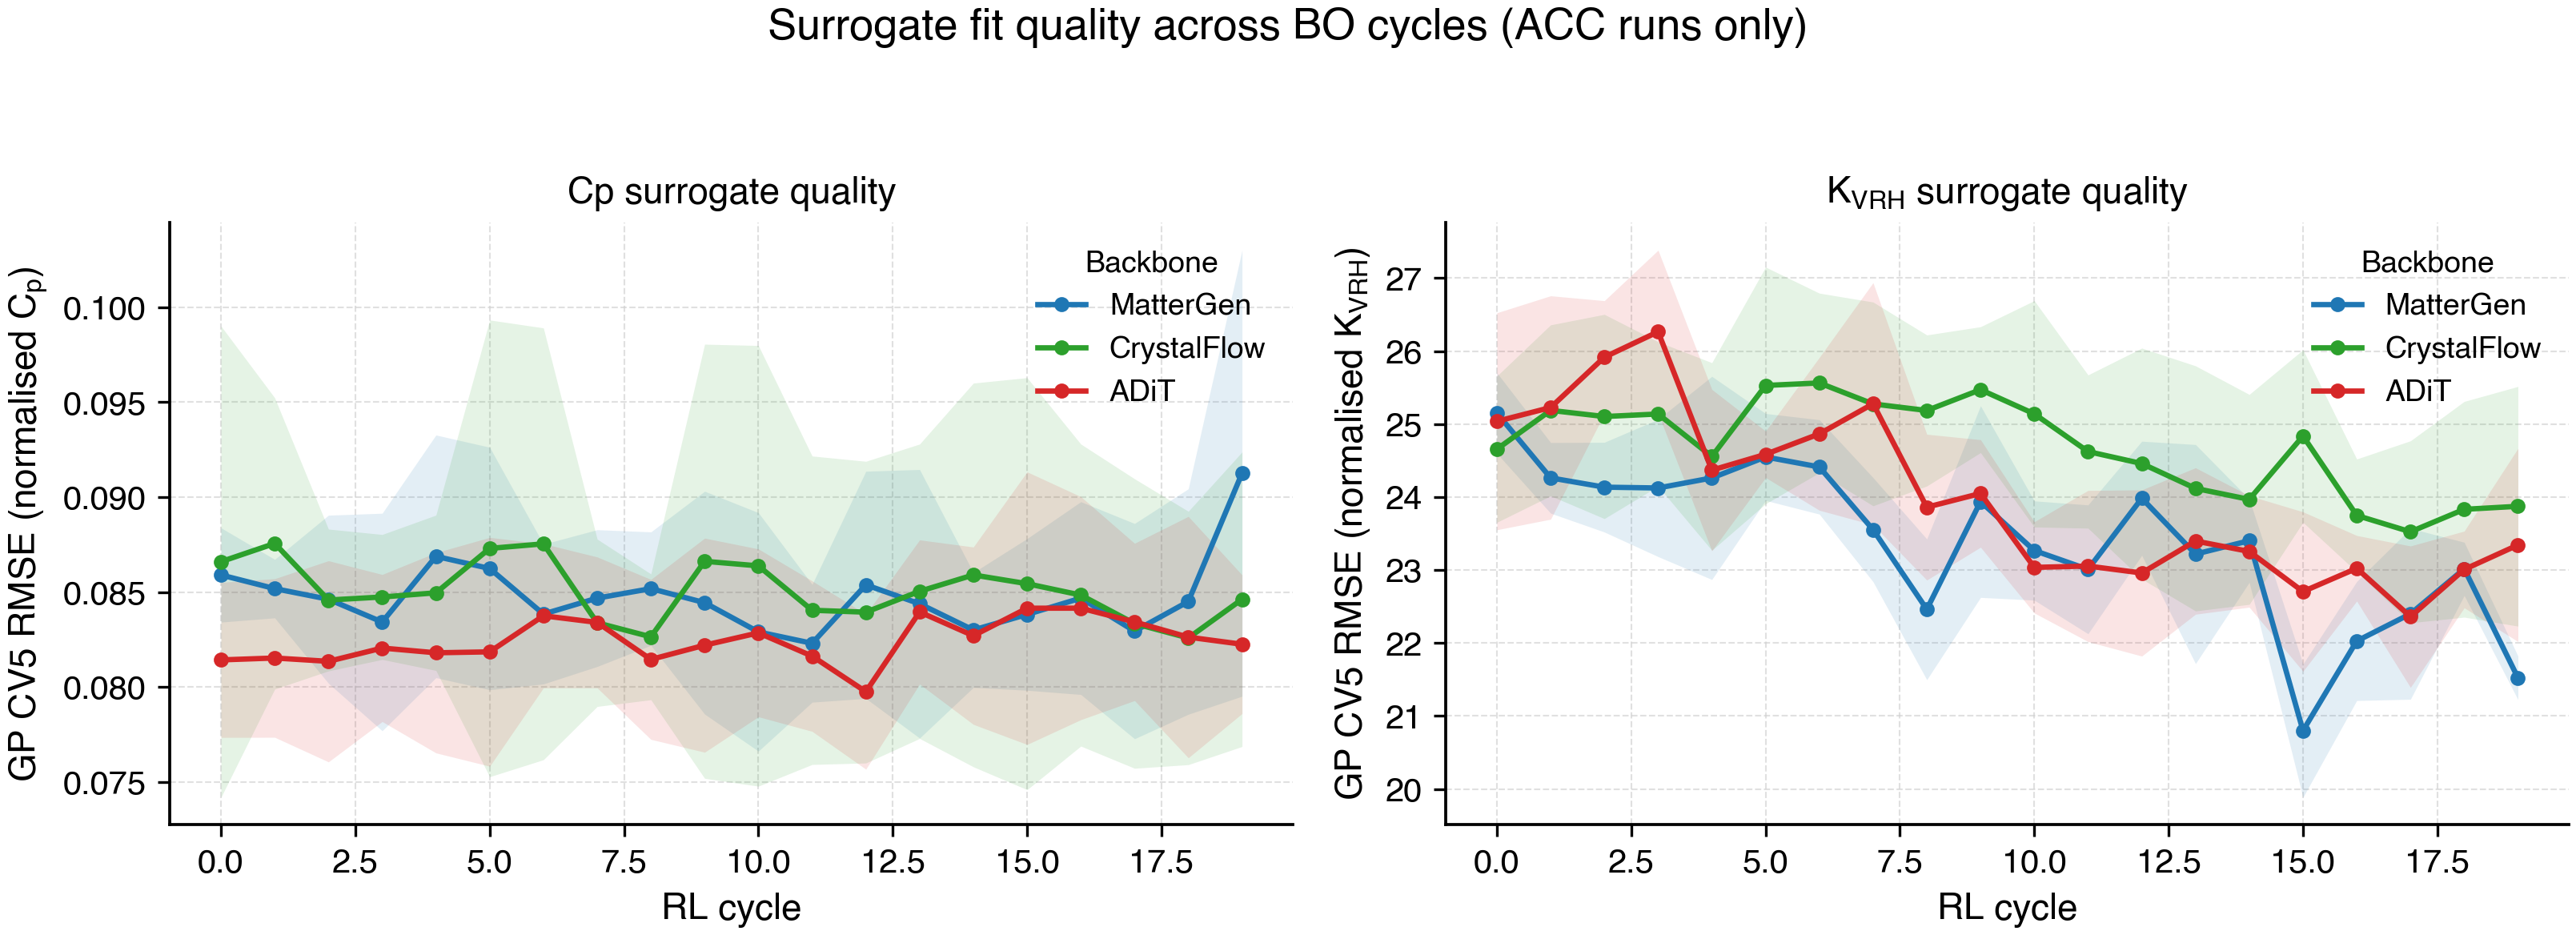
\includegraphics[width=\textwidth]{figures/fig_bogen_surrogate_quality.png}
    \caption{GP CV5 RMSE (normalised property scale) per RL cycle, ACC runs only, mean $\pm$ std across 5 seeds. CV5 is computed on the GP's accumulated oracled training set (16 points at cycle~0, growing to 92 by cycle 19), not on held-out fresh diffusion proposals. The flatness across cycles indicates that the loop does not break the GP's self-consistency as the training pool grows; it does not directly demonstrate generalisation to unseen candidates.}
    \label{fig:closed_loop_surrogate}
\end{figure*}

\FloatBarrier
\subsubsection{Oracle-Call Savings from the GP Gate}
\label{sec:cl_oracle}

The GP gate's practical payoff is that it caps the number of expensive oracle calls per cycle at $K=4$ regardless of how many candidates pass the SUN filter, replacing the rest with cheap GP-$\mu$ pseudo-evaluations.
Figure~\ref{fig:closed_loop_oracle_savings} compares cumulative oracle calls per run between BASE (every SUN-survivor goes to the oracle) and ACC (top-$K=4$ only) for both targets.
ACC's curve is the same straight line for every backbone---16 oracle calls for the warm-start at cycle 0, then 4 per cycle, totalling 92 calls per 20-cycle run.
BASE's curve depends on each backbone's SUN-survival rate.

Total oracle calls per run, 5-seed mean: for $C_p$, BASE/ACC is 169/92 in MatterGen ($1.83\times$ saving), 49/70 in CrystalFlow ($0.69\times$, i.e.\ ACC actually costs more), and 70/84 in ADiT ($0.83\times$); for $K_{\text{VRH}}$, BASE/ACC is 320/92 in MatterGen ($3.47\times$), 124/68 in CrystalFlow ($1.83\times$), and 206/83 in ADiT ($2.49\times$).
The pattern is consistent: where SUN survival per cycle exceeds $K=4$ (MatterGen on both targets, all backbones on $K_{\text{VRH}}$), the gate pays off; where survival is below $K$ (CrystalFlow and ADiT on $C_p$, where the unfiltered REINFORCE produces few stable+unique+novel candidates), BASE is naturally throttled and ACC's fixed $K$ raises rather than lowers the call count.
The trade-off in those low-throughput cases is not a saving in oracle calls but a saving in candidate quality: the gate forces a top-$K$ selection by EI\,+\,DPP rather than letting whatever survives SUN drift through to the oracle.

\begin{figure*}[!htb]
    \centering
    
\includegraphics[width=\textwidth]{figures/fig_bogen_oracle_savings.png}
    \caption{Cumulative oracle calls per closed-loop run, 5-seed mean $\pm$ std. ACC's straight line at +4 per cycle (after a warm-start of 16) reflects the fixed top-$K=4$ gate. BASE varies with each backbone's SUN-survival rate. The gate saves oracle calls for backbones with high SUN survival (MatterGen on both targets, all backbones on $K_{\text{VRH}}$, $1.8$--$3.5\times$ reduction); for low-survival backbones on $C_p$, ACC's fixed $K$ slightly raises the call count, with the trade-off being that the candidates picked are EI\,+\,DPP-selected rather than arbitrary SUN survivors.}
    \label{fig:closed_loop_oracle_savings}
\end{figure*}

\FloatBarrier
\subsubsection{Crystal-System Distribution of Generated Top Structures}
\label{sec:cl_crystal_systems}

The space groups of the top-3 candidates per run reveal a strong asymmetry across backbones (Figure~\ref{fig:closed_loop_spacegroup}).
For $C_p$, CrystalFlow and ADiT both produce more than half of their top structures in triclinic and monoclinic systems---the lowest-symmetry crystal classes---while MatterGen splits more evenly, contributing the bulk of the orthorhombic and tetragonal hits.
This is consistent with each prior's training distribution: MatterGen is trained on Materials Project ground-state structures (symmetry-rich), whereas the latent and flow priors more often emerge from optimisation in low-symmetry space.
For $K_{\text{VRH}}$ (Supporting Information) the dominance of low-symmetry systems persists, but cubic and hexagonal structures are over-represented relative to $C_p$, reflecting the well-known correlation between high bulk modulus and densely packed cubic/hexagonal lattices.
Splitting by policy (right panel) shows that the GP gate (ACC) does not bias the loop towards any particular crystal system---both BASE and ACC produce the same broad triclinic/monoclinic dominance, so the GP is screening on the property rather than on geometric proxies.

\begin{figure*}[!htb]
    \centering
    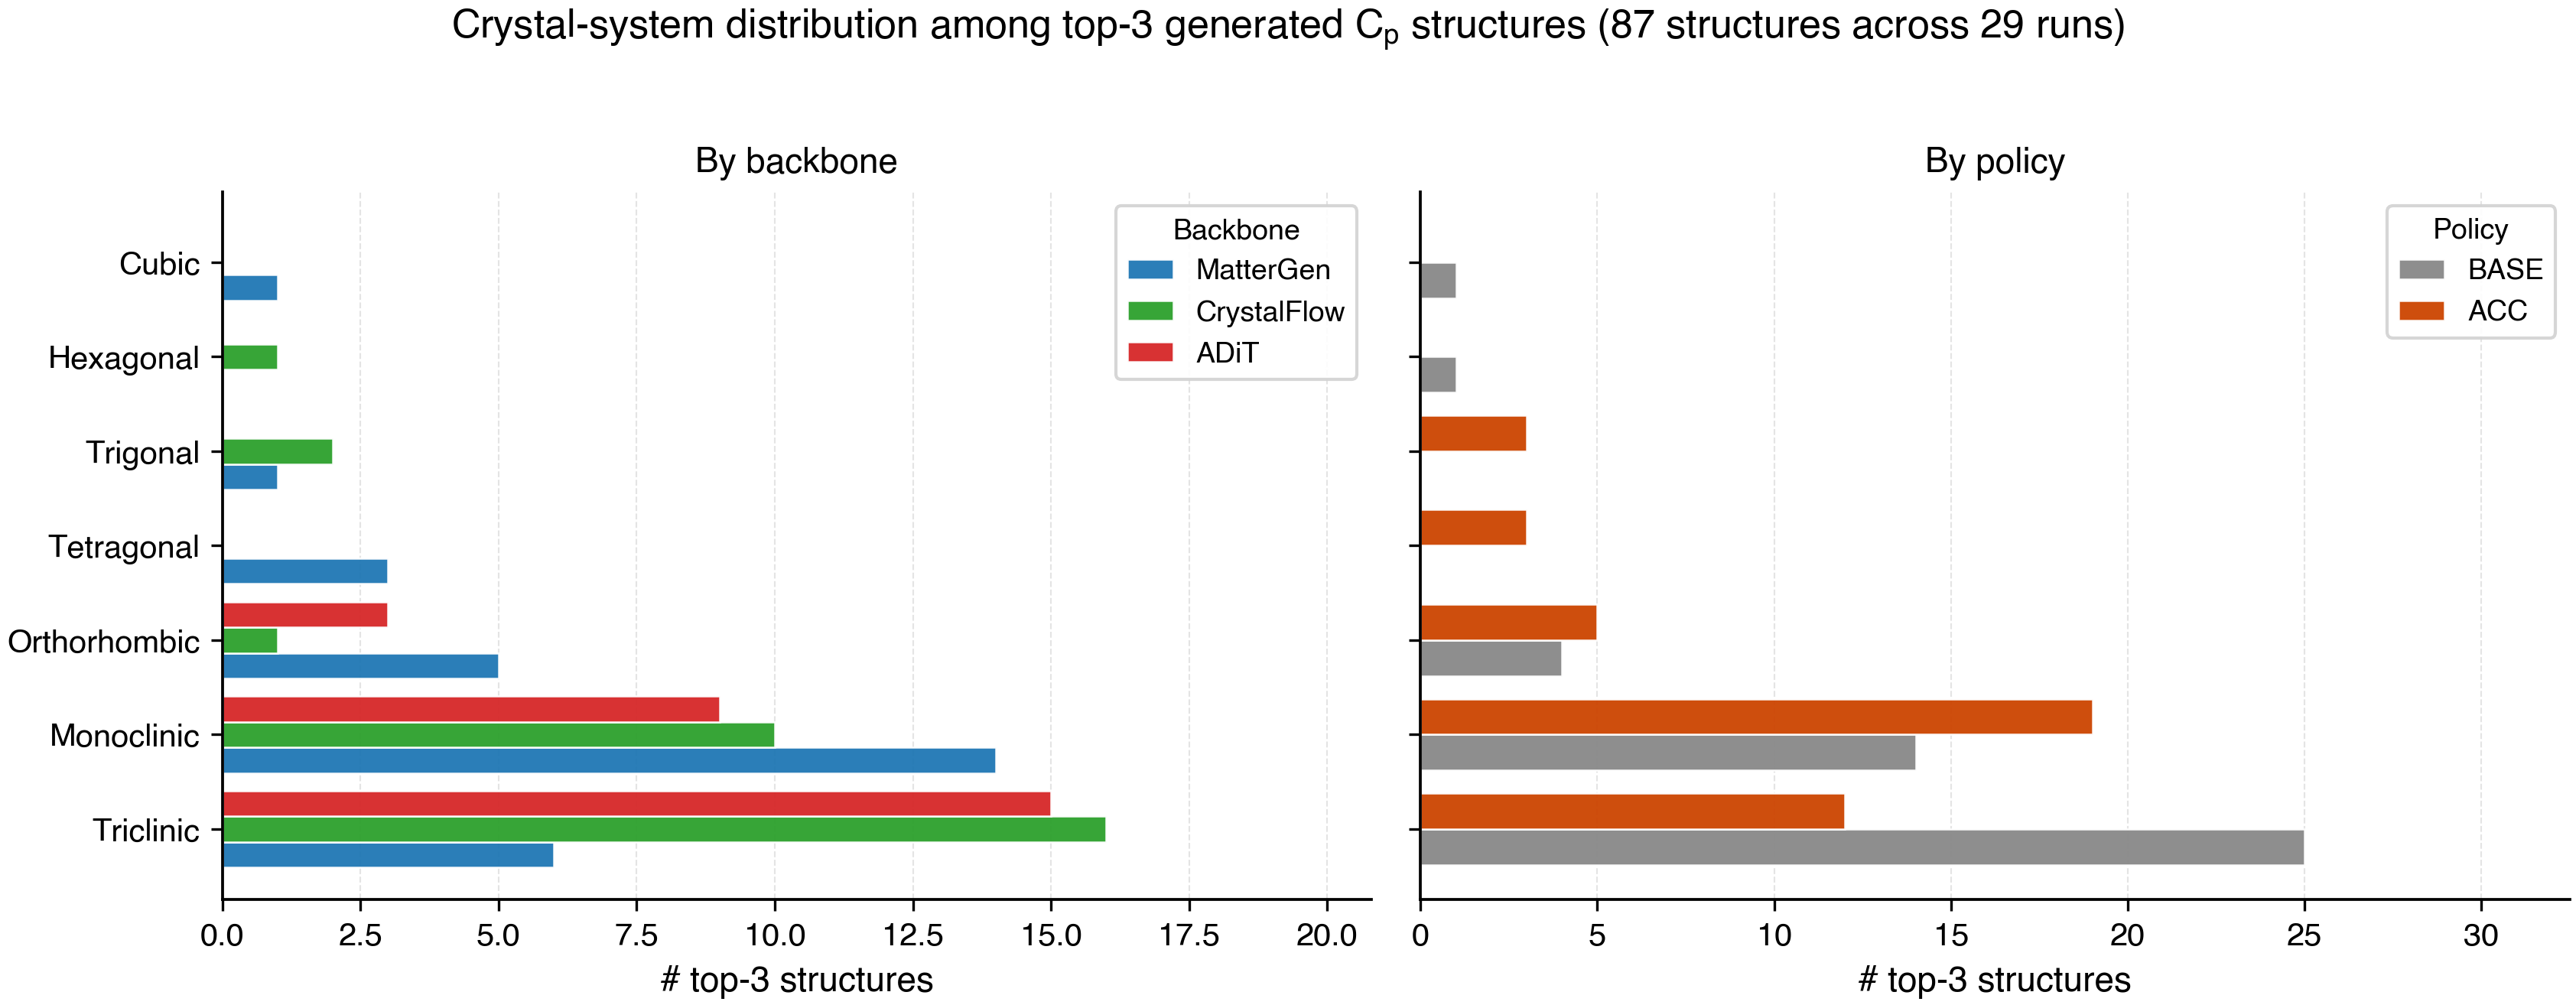
\includegraphics[width=\textwidth]{figures/fig_bogen_spacegroup_dist_cp.png}
    \caption{Crystal-system distribution among top-3 generated $C_p$ structures (87 structures across 30 runs). Left: by backbone. Right: by policy. CrystalFlow and ADiT skew strongly towards low-symmetry (triclinic, monoclinic) systems; MatterGen is the only backbone producing tetragonal hits; the BASE-vs-ACC split is balanced across systems, so the GP gate is property-driven, not geometry-driven. The matching $K_{\text{VRH}}$ panel is in the Supporting Information.}
    \label{fig:closed_loop_spacegroup}
\end{figure*}

\FloatBarrier
\subsubsection{Per-Backbone Summary}
\label{sec:cl_per_model}

Figure~\ref{fig:closed_loop_per_model} consolidates the headline numbers per backbone across all 30 runs.
Best-value bars (left column) split BASE vs.\ ACC: MatterGen and CrystalFlow both hit the 2.0~J/g/K reward ceiling (oracle-imposed cap, attained on a few seeds) while ADiT plateaus at 1.28~J/g/K; for $K_{\text{VRH}}$, ADiT's 375~GPa hit pulls its best-value bar above MatterGen's 340 and CrystalFlow's 336~GPa.
Mean top-3 (right column) is the more honest comparator because best-of-30 picks up lucky seeds: on $C_p$ the three backbones land at 1.11~$\pm$~0.56, 0.89~$\pm$~0.40, and 0.80~$\pm$~0.18~J/g/K---differences smaller than the within-backbone seed spread.
On $K_{\text{VRH}}$ the corresponding means are 273~$\pm$~37, 224~$\pm$~43, and 259~$\pm$~45~GPa, again with overlapping error bars.
Novelty against the warm-start seed pool is uniform across backbones at 100\% for $C_p$ and 96.7\% for $K_{\text{VRH}}$, so we report it verbally rather than as a separate panel; details and the formula-level analysis are in Section~\ref{sec:cl_novelty}.
The ACC-vs-BASE lift on best-of-30 is consistent in MatterGen and ADiT (Section~\ref{sec:cl_curves}) but never large enough to outweigh seed variance, so we report it as a trend rather than a measured difference.

\begin{figure*}[!htb]
    \centering
    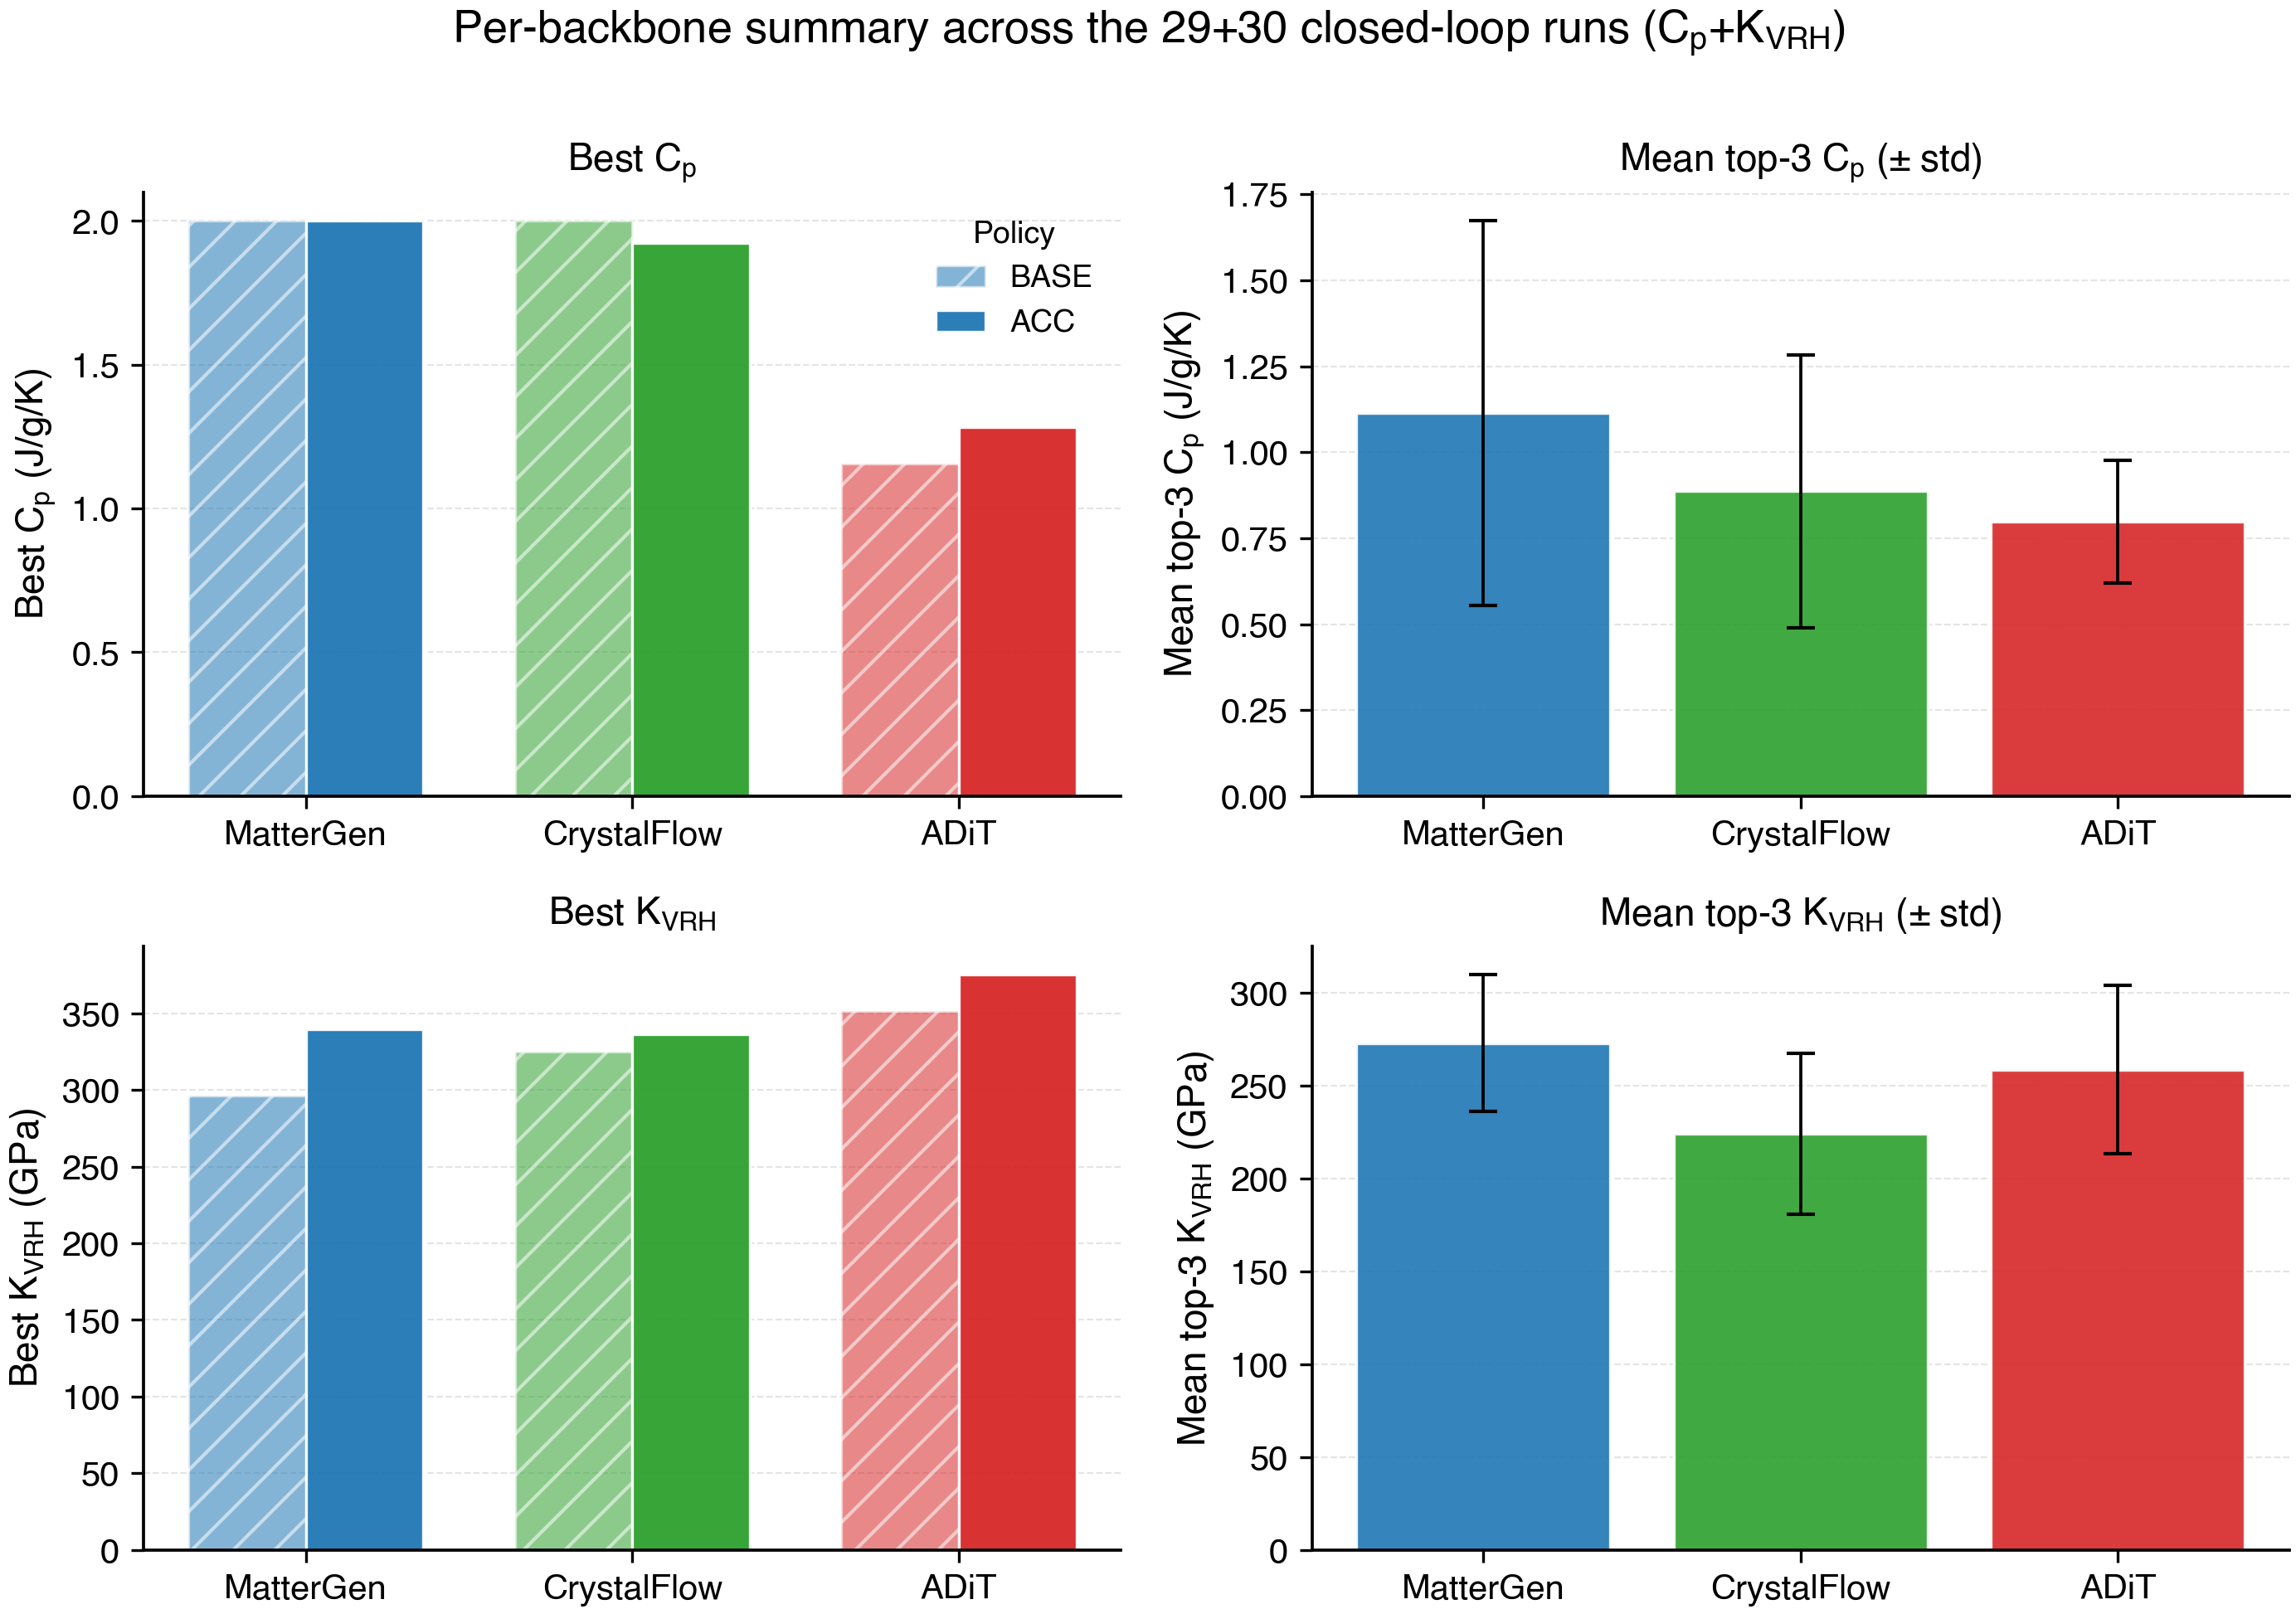
\includegraphics[width=0.85\textwidth]{figures/fig_bogen_per_model_summary.png}
    \caption{Per-backbone summary across the 30 closed-loop runs. Left column: best property value (hatched = BASE, solid = ACC). Right column: mean top-3 value $\pm$ std across runs. Top row: $C_p$. Bottom row: $K_{\text{VRH}}$. The best-value spread across backbones is small once seed variance is taken into account; ACC's lift over BASE is consistent but modest. Novelty rates against the warm-start seed pool are 100\% ($C_p$) and 96.7\% ($K_{\text{VRH}}$) for all three backbones (Section~\ref{sec:cl_novelty}).}
    \label{fig:closed_loop_per_model}
\end{figure*}

\FloatBarrier
\subsubsection{Novelty vs.\ the Warm-Start Seed Pool}
\label{sec:cl_novelty}

A natural worry is that the loop is retrieving the structures we used to warm-start the GP rather than producing new ones.
We checked this with \texttt{StructureMatcher}~\cite{pymatgen2013} at default tolerances.
For $C_p$, none of the 87 top-3 structures (aggregated across all 30 runs) shares a reduced formula with the seed pool, and zero pass strict matching.
For $K_{\text{VRH}}$, 3 of 90 share a reduced formula but again zero pass strict matching.
The GP is acting as a property prior, not as memory.

Figure~\ref{fig:closed_loop_zoo} shows the top-20 structures per target, borders coded by backbone.
The compositions split along physical lines: light-element binaries and ternaries (Li, Mg, Na, F, O) for $C_p$, transition-metal carbides, nitrides, and borides (Mo, W, Os, Re) for $K_{\text{VRH}}$---roughly what each property's known physical drivers would predict.

\begin{figure*}[!htb]
    \centering
    \begin{subfigure}[t]{0.48\textwidth}
        \centering
        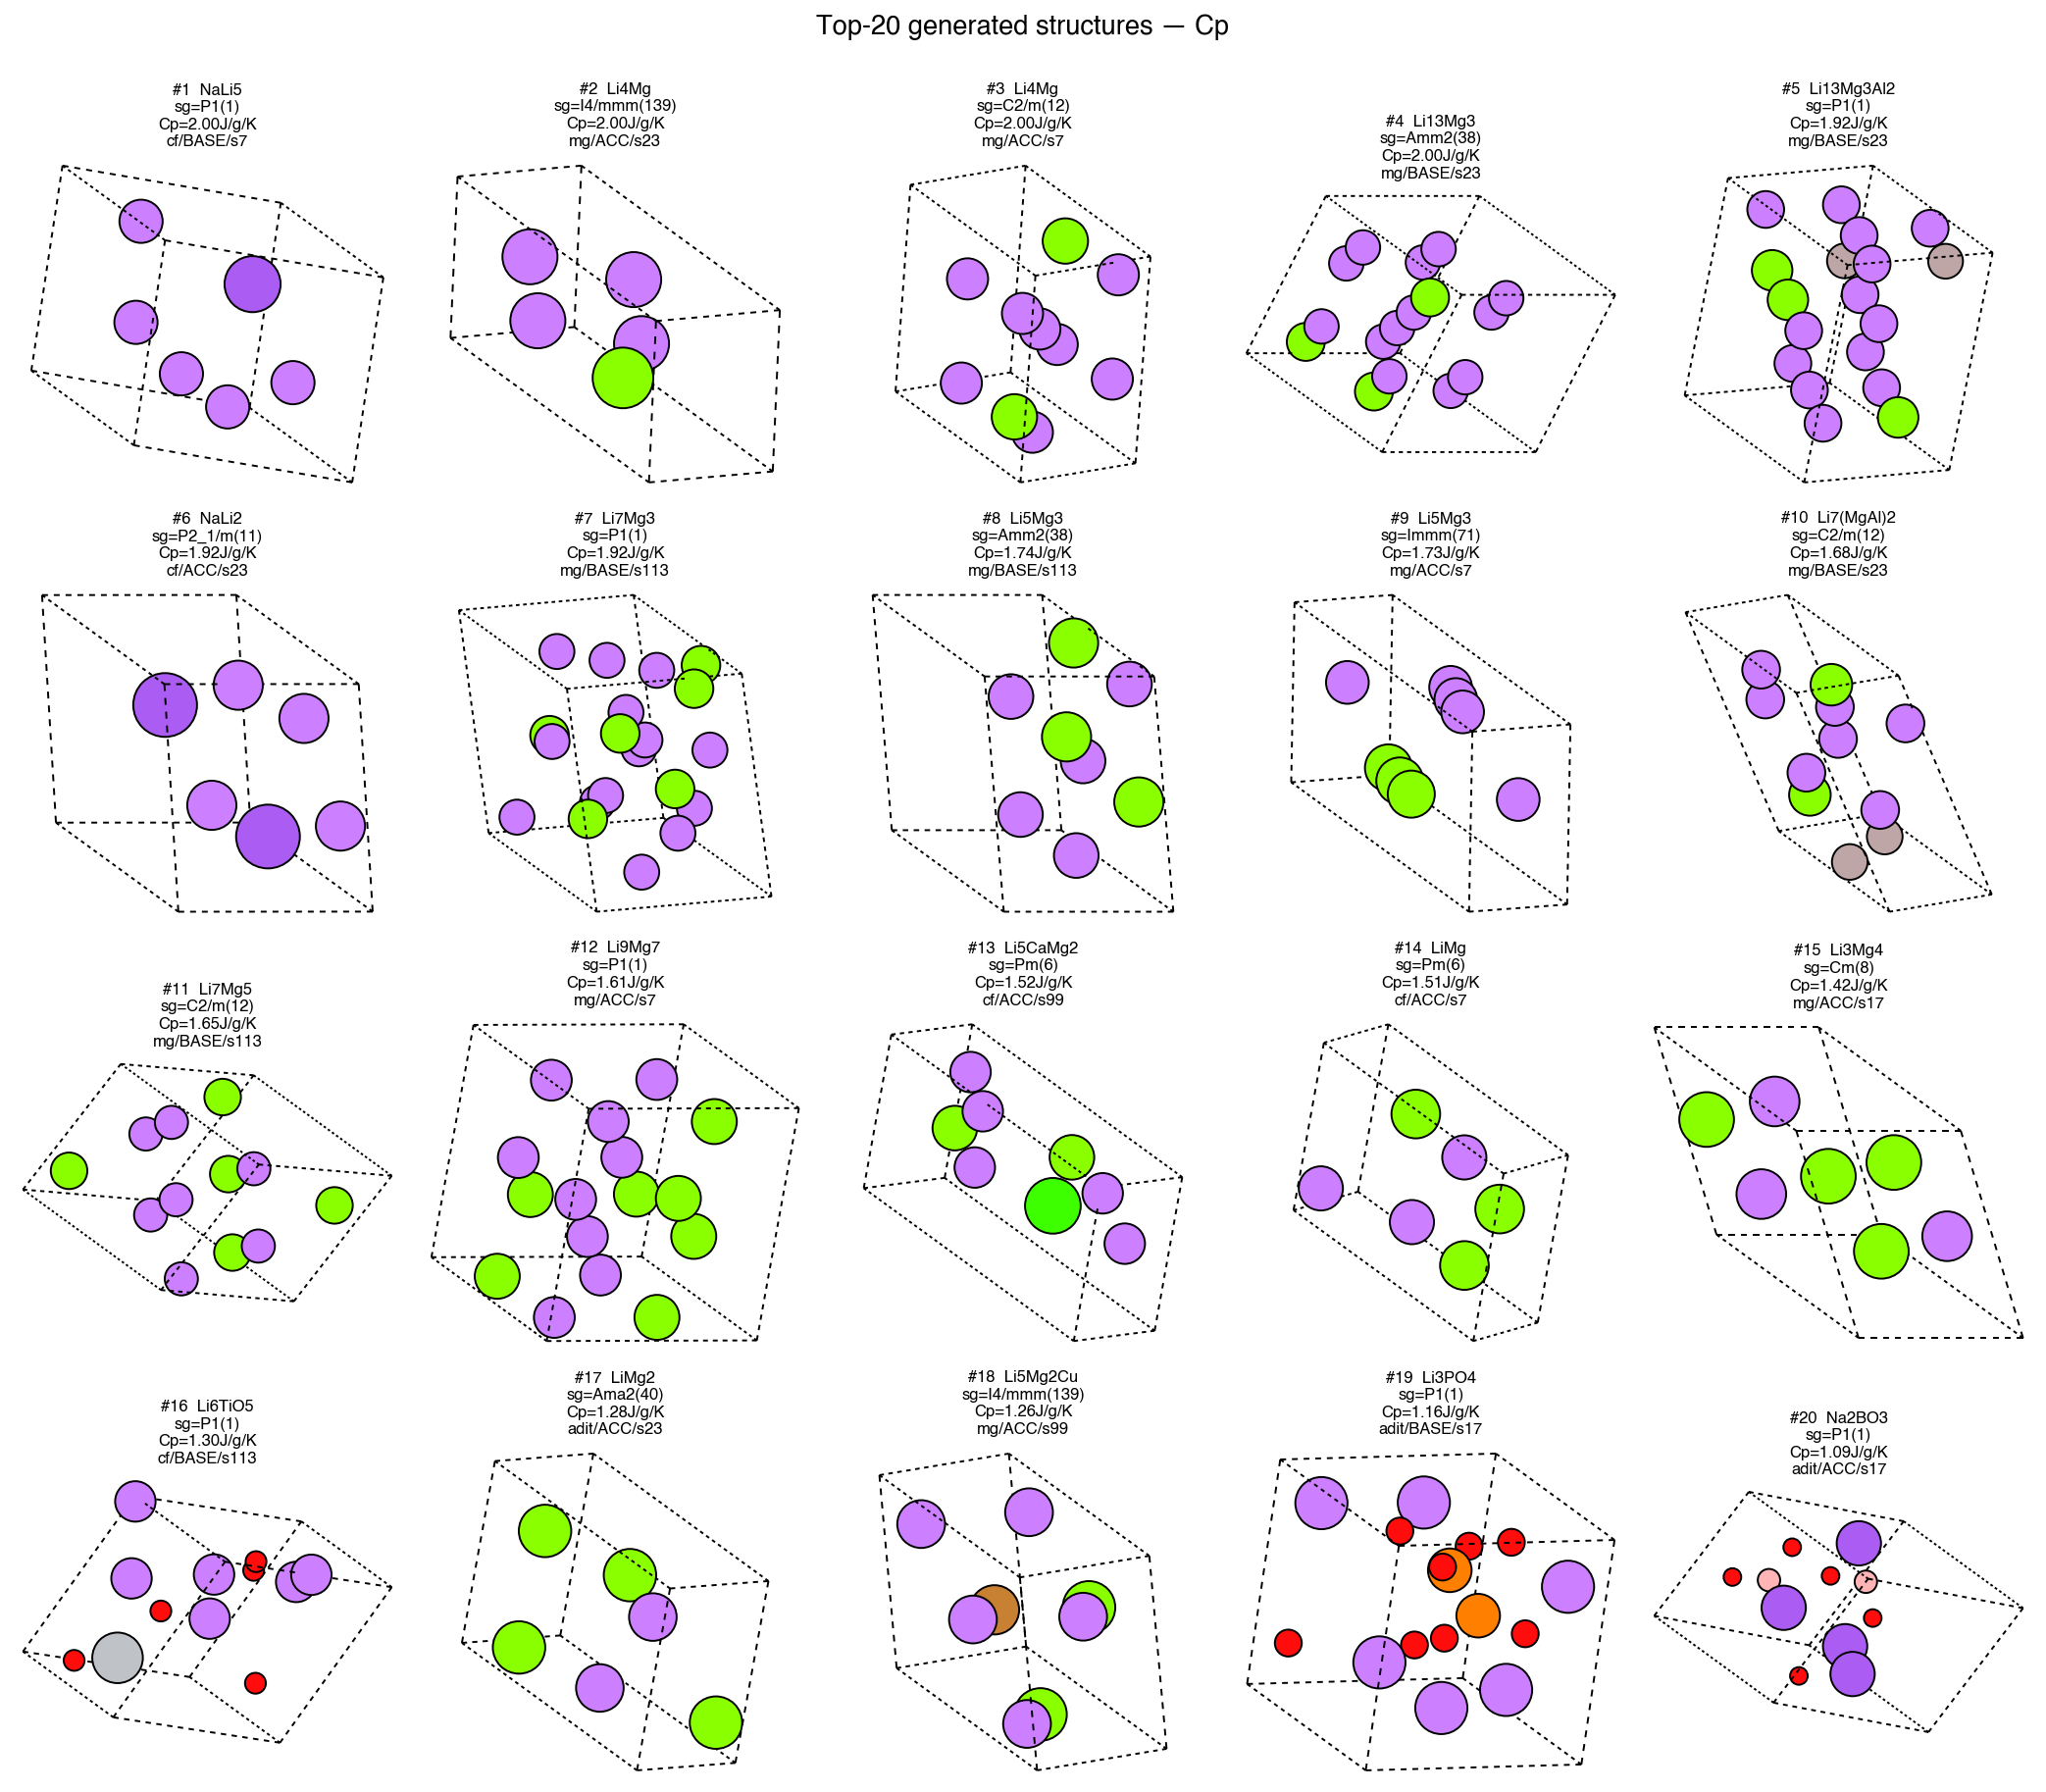
\includegraphics[width=\textwidth]{figures/fig_bogen_structure_zoo_cp.png}
        \caption{Heat capacity ($C_p$)}
    \end{subfigure}
    \hfill
    \begin{subfigure}[t]{0.48\textwidth}
        \centering
        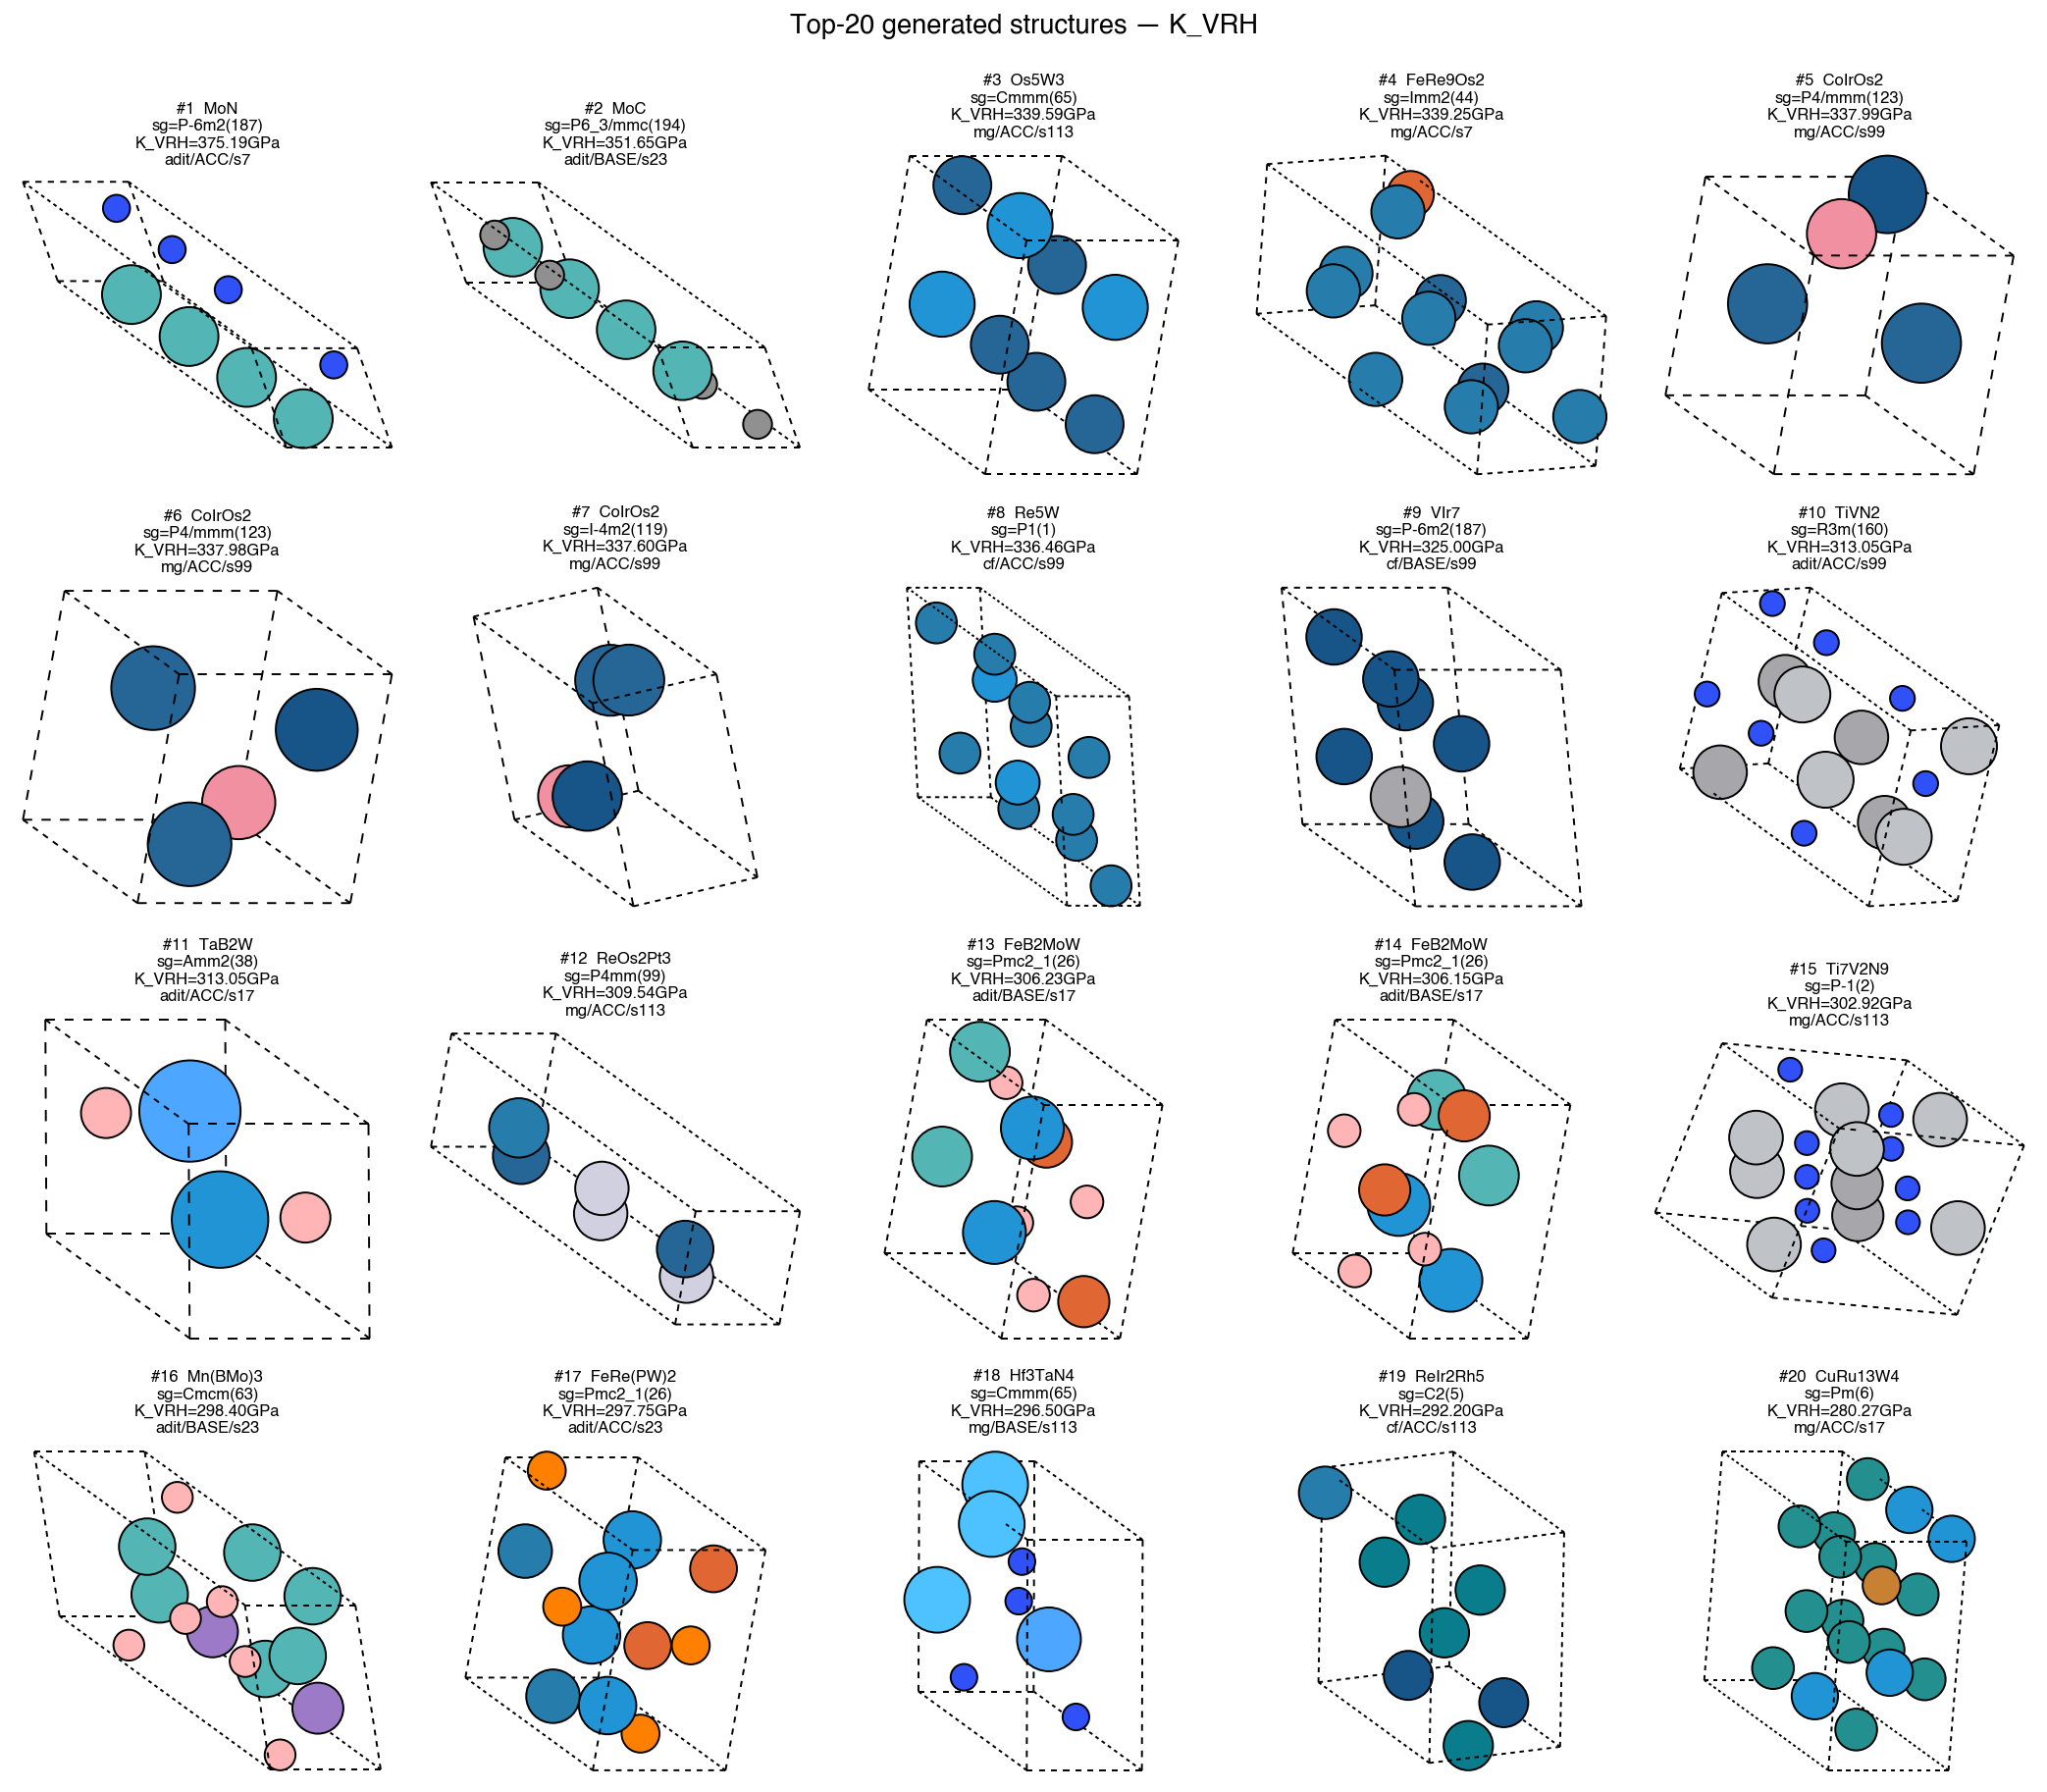
\includegraphics[width=\textwidth]{figures/fig_bogen_structure_zoo_bm.png}
        \caption{Bulk modulus ($K_{\text{VRH}}$)}
    \end{subfigure}
    \caption{Top-20 generated structures per target (4$\times$5 grid), ranked by the oracle. Border colour: blue = MatterGen, green = CrystalFlow, red = ADiT. Each panel reports formula, space group, target value, and the originating (cycle, seed). None pass strict \texttt{StructureMatcher} against the warm-start seed pool.}
    \label{fig:closed_loop_zoo}
\end{figure*}

\subsubsection{What the Probe Does and Does Not Establish}
\label{sec:cl_caveats}

Five seeds, three pretrained backbones, and a learned (not DFT) oracle are enough to draw a few methodological conclusions, not to crown a winning generator.
The loop closes across three architecturally distinct priors with internally self-consistent GP fits across cycles; ACC outperforms BASE in two of three backbones for both targets; the generator does not retrieve memorised seeds; and the crystal-system mix follows each prior's bias.
What the probe does \emph{not} establish is a final ranking of MatterGen vs.\ CrystalFlow vs.\ ADiT.
The cross-seed variance, especially in CrystalFlow, is too large for that, and our oracle is itself a learned surrogate.
A second gap is in the surrogate diagnostics themselves: the only GP-quality signal we log is CV5 on the accumulated training set (Section~\ref{sec:cl_surrogate}), which is a self-consistency check rather than a generalisation test on fresh diffusion proposals.
A definitive comparison would therefore require more seeds per cell, fine-tuning of the diffusion priors against the target property, DFT validation of the top-K hits per backbone, and a held-out RMSE---measured on each cycle's fresh candidates before they reach the gate---to track whether the GP generalises rather than just stays self-consistent.

\section{Discussion}
\label{sec:discussion}

\subsection{Why ORB Embeddings Win}
\label{sec:why_orb}

ORB's consistent dominance across all three datasets, all surrogates, and nearly every individual property demands explanation.
On the elastic tensor dataset, ORB achieves $\bar{R}^2 = 0.803$ with the GP---a margin of $\Delta R^2 \approx 0.07$ over UMA (0.734) and MACE (0.731).
On the dielectric dataset, ORB\,+\,DGP at PCA\,=\,10 reaches $\bar{R}^2 = 0.336$, outperforming the next best (MACE\,+\,DGP, 0.239) by nearly 0.10 absolute points.
On the phonon dataset, the gap narrows to $\Delta R^2 \approx 0.03$ (ORB 0.303 vs.\ UMA 0.272), yet ORB never cedes the top position.
We attribute this universality to three factors.

First, \emph{pre-training data scale and diversity}.
ORB was trained on the combined Alexandria and MPTrj datasets, comprising approximately 120~million atomic configurations spanning most of the periodic table.
This is roughly three orders of magnitude larger than MACE-MP-0's training set ($\sim$150{,}000 structures) and gives ORB broader chemical coverage.
The analogy is instructive: just as a language model trained on all of Wikipedia produces richer sentence embeddings than one trained on a single textbook, even if both share the same architecture, the sheer diversity of ORB's pre-training corpus endows its embeddings with a more comprehensive map of chemical space.

Second, \emph{architectural design for periodic systems}.
ORB's graph attention mechanism with explicit edge features is specifically designed for crystalline materials with periodic boundary conditions.
While MACE's equivariant message passing captures many-body interactions through tensor products, ORB's attention mechanism learns which atomic interactions matter most, effectively performing a soft feature selection during pre-training.
This architectural difference may explain why ORB's advantage is largest on the elastic dataset, where long-range elastic interactions between atoms contribute to bulk properties.

Third, \emph{embedding compactness}.
When we reduce ORB embeddings via PCA, even the first 10~components capture sufficient variance to outperform SOAP at PCA\,=\,50 on the elastic dataset (ORB: $\bar{R}^2 = 0.736$ vs.\ SOAP: $\bar{R}^2 = 0.445$).
On the phonon dataset, the same comparison holds: ORB at PCA\,=\,10 achieves $\bar{R}^2 = 0.281$ versus SOAP's best of 0.235 at PCA\,=\,50.
This implies that ORB's raw embedding space is more structured and informative, with the principal axes aligning naturally with property-relevant structural variation.

The near-parity between UMA and MACE across datasets ($\bar{R}^2 \approx 0.73$ for both at GP\,+\,PCA\,=\,50 on elastic; $\bar{R}^2 \approx 0.27$ on phonon) is also noteworthy.
Despite different architectures (eSCN-based vs.\ equivariant message passing) and different pre-training data, they converge on similar embedding quality.
This convergence hints at a ``representational ceiling'' that can only be broken by substantially larger pre-training corpora---precisely the advantage that ORB exploits.

One notable exception to ORB dominance is the dielectric dataset under GP and MTGP, where SOAP achieves higher \Rtwo{} than ORB (SOAP\,+\,MTGP: $\bar{R}^2 = 0.177$ vs.\ ORB\,+\,MTGP: 0.121; SOAP\,+\,GP: 0.132 vs.\ ORB\,+\,GP: 0.096).
This reversal occurs because dielectric response depends heavily on local bonding chemistry and electronic polarisability---features that SOAP's explicit encoding of local environments captures, while foundation model embeddings, optimised for energy and forces, may under-represent.
However, ORB recovers its lead under DGP ($\bar{R}^2 = 0.336$ vs.\ SOAP's $-0.016$), and critically, ORB's Spearman correlations are consistently higher ($\bar{\rho} = 0.746$--$0.778$ vs.\ SOAP's 0.019--0.583), indicating that ORB preserves material \emph{rankings} even when its absolute \Rtwo{} is lower.

\FloatBarrier
\subsection{PCA Sensitivity and DGP Configuration}
\label{sec:pca_sensitivity_discussion}

PCA dimensionality is a key hyperparameter in our pipeline, and its effect varies substantially across surrogates and datasets.
The GP and MTGP are generally robust to PCA dimension: increasing from 10 to 50 produces monotonic improvement or near-plateau on all datasets.
On the elastic data, GP\,+\,ORB improves from $\bar{R}^2 = 0.736$ (PCA\,=\,10) to 0.803 (PCA\,=\,50), while on the phonon data the equivalent gain is 0.281 to 0.303.
MACE is the most PCA-robust featuriser on the elastic dataset, varying by only $\Delta R^2 = 0.005$ across PCA levels.
SOAP benefits the most from higher PCA dimensions: on the elastic data, its $\bar{R}^2$ more than doubles from 0.197 (PCA\,=\,10) to 0.445 (PCA\,=\,50), reflecting the high intrinsic dimensionality of the SOAP descriptor.

The DGP requires more careful PCA selection but rewards it with strong performance.
On the elastic dataset, ORB\,+\,DGP at PCA\,=\,25 achieves the single best averaged $\bar{R}^2$ of 0.807---surpassing all GP and MTGP configurations.
On the dielectric dataset, DGP\,+\,ORB at PCA\,=\,10 achieves $\bar{R}^2 = 0.336$, substantially outperforming both GP ($0.096$) and MTGP ($0.121$).
On the phonon dataset, DGP\,+\,ORB at PCA\,=\,25 matches the GP ($\bar{R}^2 = 0.302$ vs.\ $0.303$).
Figure~\ref{fig:cross_surrogate} summarises this pattern: the DGP delivers the best \Rtwo{} on two of three datasets (elastic and dielectric), while the GP leads on the phonon dataset.
These results demonstrate that the DGP is a powerful surrogate when properly configured, not a fragile one.

\begin{figure}[H]
    \centering
    
\includegraphics[width=\columnwidth]{figures/fig_cross_surrogate_r2_pptx.png}
    \caption{Best averaged \Rtwo{} per surrogate across all three datasets (ORB descriptor, $\ntrain = 500$, best PCA per surrogate). The DGP achieves the highest \Rtwo{} on the elastic and dielectric datasets, while the GP leads on the phonon dataset. This complementary pattern supports using DGP for non-linear properties and GP as a robust default.}
    \label{fig:cross_surrogate}
\end{figure}

The learning curves for the dielectric and phonon datasets (Figures~\ref{fig:learning_curves_dielectric} and~\ref{fig:learning_curves_phonon}) add a temporal dimension to this analysis.
On the dielectric dataset, the DGP's \Rtwo{} remains relatively stable across training sizes while the GP and MTGP actually \emph{degrade}---a consequence of the heavy-tailed property distributions introducing more outliers as the dataset grows.
On the phonon dataset, all surrogates improve modestly, with the DGP catching up to the GP at $\ntrain = 500$.
These trends confirm that the DGP's non-linear capacity is most valuable when the property distribution is complex or when the training set is large enough to support its variational parameters.

The DGP's sensitivity to PCA dimension is a practical consideration rather than a fundamental limitation.
At PCA\,=\,50 with $\ntrain = 500$, the two-layer variational architecture must estimate $O(d^2)$ parameters in the hidden layer, pushing the data-to-parameter ratio below the threshold needed for stable ELBO optimisation.
At PCA\,$\leq$\,25, this ratio is favourable, and the DGP's non-linear feature transformations can capture structure--property relationships that the linear GP cannot.
This is most evident for elastic anisotropy, where DGP\,+\,ORB achieves $R^2 = 0.746$ versus GP\,+\,ORB's $0.582$---a 0.16-point advantage attributable to the DGP's ability to model complex, non-linear mappings.

\emph{Practical guideline:} Treat PCA dimension as a first-class hyperparameter when using DGP.
The combination PCA\,$\in\{10, 25\}$ with $\ntrain \geq 300$ yields strong, reliable results across all three datasets.
For GP and MTGP, PCA\,=\,50 is a safe default.

\FloatBarrier
\subsection{Multi-Task GP: When Correlation Helps}
\label{sec:mtgp_discussion}

The MTGP's performance across our three datasets reveals an instructive pattern about when multi-task learning adds value for materials property prediction.

On the elastic dataset, MTGP consistently underperforms the independent GP: MTGP\,+\,ORB achieves $\bar{R}^2 = 0.780$ versus the GP's 0.803.
This is surprising given the strong correlations among elastic properties---$K_{\text{Voigt}}$, $K_{\text{VRH}}$, and $K_{\text{Reuss}}$ are three averaging schemes of the same underlying elastic tensor, and the shear modulus variants are similarly related.
We identify three contributing factors.
The ICM kernel must estimate a $T \times T$ task correlation matrix (where $T = 8$ for the elastic dataset), adding $T(T-1)/2 = 28$ parameters that introduce regularisation overhead.
The heterogeneous property scales (bulk modulus in GPa vs.\ Poisson's ratio as a dimensionless ratio) can destabilise the shared lengthscale.
And when each property is already well-predicted independently---as ORB\,+\,GP demonstrates---the marginal improvement from multi-task learning diminishes, a regime known as ``negative transfer''~\cite{yamada2019predicting}.

On the phonon dataset, however, MTGP is essentially tied with the GP: $\bar{R}^2 = 0.302$ vs.\ 0.303, with $\bar{\rho} = 0.830$ vs.\ 0.824.
Here the MTGP may benefit from the correlation between eps\_electronic and eps\_total (both measuring dielectric response, differing only by the ionic contribution) and between the dielectric constants and the phonon DOS peak (which reflects the lightest-atom vibrations that also influence dielectric response).
With only 3~tasks, the correlation matrix adds just 3~extra parameters, keeping the overhead manageable.

On the dielectric dataset, MTGP\,+\,SOAP achieves $\bar{R}^2 = 0.177$ versus SOAP\,+\,GP's $0.132$---a 34\% relative improvement.
This suggests that multi-task learning can compensate for weaker featurisers when property correlations are strong (band gap and refractive index are physically related through the electronic structure).
With ORB, the MTGP benefit is smaller but still present in terms of Spearman correlation ($\bar{\rho} = 0.773$ vs.\ 0.746).

The emerging pattern is that MTGP helps most when the number of tasks is small ($T \leq 4$), the per-task prediction is weak (leaving room for multi-task transfer to fill in), and properties share a common physical origin.
It helps least when tasks are numerous, individually well-predicted, or span disparate physical phenomena.

\FloatBarrier
\subsection{Dataset Difficulty Spectrum}
\label{sec:difficulty_spectrum}

The three datasets span a wide difficulty spectrum that illuminates the fundamental limits of geometric embedding-based surrogates.
Elastic properties are the easiest ($\bar{R}^2$ up to 0.807), phonon dielectric properties are intermediate ($\bar{R}^2$ up to 0.303), and electronic dielectric properties occupy the hardest regime ($\bar{R}^2$ up to 0.336 overall, but with individual properties ranging from $R^2 = 0.852$ for band gap to $R^2 < 0$ for polycrystalline electronic dielectric constant).

This hierarchy has a clear physical explanation grounded in the ``information distance'' between crystal geometry and the target property.

\textbf{Elastic properties} depend primarily on bond stiffness, atomic packing density, and nearest-neighbour distances---precisely the features that geometric embeddings encode most directly.
Bulk modulus ($K$) is an isotropic measure of resistance to uniform compression, and its high predictability ($R^2 > 0.91$ for all three Voigt/VRH/Reuss variants) confirms that foundation model embeddings capture local bonding information effectively.
The energy landscape for elastic deformation is smooth and dominated by harmonic contributions near equilibrium, making it well-suited to the linear kernel of the GP.
Shear modulus ($G$) introduces directional dependence ($R^2 = 0.78$--$0.83$), while elastic anisotropy and Poisson's ratio ($R^2 = 0.66$--$0.75$) require global structural understanding beyond local atomic environments.

\textbf{Phonon properties} involve the vibrational modes of the crystal lattice, which depend on the potential energy surface (PES) beyond the harmonic regime.
The last phonon DOS peak is well-predicted ($R^2 = 0.911$) because the highest-frequency vibrational mode is strongly determined by the lightest atoms and their bond stiffness---information directly accessible from geometric embeddings.
However, the dielectric constants derived from phonon calculations (eps\_electronic, eps\_total) yield $R^2 \approx -0.001$ for all methods, reflecting the fact that dielectric response involves the collective, many-body polarisation of the electron density, which is far removed from geometric descriptors.
The high Spearman correlations ($\rho = 0.930$ for eps\_electronic) indicate that the \emph{ordering} is preserved even when absolute predictions fail.

\textbf{Dielectric properties} require electronic structure information---band gaps, orbital hybridisation, and many-body screening effects---that geometric embeddings capture only indirectly through correlations between bonding geometry and electronic structure.
Band gap is reasonably predictable ($R^2 = 0.852$) because it correlates with electronegativity differences, bond ionicity, and coordination environment, all of which leave geometric fingerprints.
The polycrystalline dielectric constants ($R^2 < 0$), however, depend on the full frequency-dependent polarisability tensor, which has no simple geometric proxy.

This difficulty gradient has practical implications: for properties near the ``geometric'' end of the spectrum (mechanical, thermal conductivity, phonon frequencies), our pipeline is immediately applicable.
For properties near the ``electronic'' end (optical gaps, dielectric response, magnetic moments), the Spearman correlations suggest that the surrogates can still guide Bayesian optimisation through reliable ranking, but absolute property predictions require electronic-structure-aware embeddings or hybrid featurisation strategies.

\FloatBarrier
\subsection{Ranking Accuracy Matters More Than Regression Accuracy}
\label{sec:spearman_r2}

We argue that the most practically important finding of this benchmark is the systematic and large discrepancy between Spearman rank correlation ($\rho$) and coefficient of determination (\Rtwo{}) across all three datasets.
This discrepancy fundamentally changes how we should evaluate surrogates for materials design, and suggests that the dielectric and phonon surrogates are far more useful than their \Rtwo{} values imply.

The numbers are striking.
On the elastic dataset, the gap is modest: $\bar{\rho} = 0.842$ vs.\ $\bar{R}^2 = 0.803$ for ORB\,+\,GP.
On the dielectric dataset, it widens: $\bar{\rho} = 0.778$ vs.\ $\bar{R}^2 = 0.336$ for ORB\,+\,DGP.
On the phonon dataset, it becomes dramatic: $\bar{\rho} = 0.824$ vs.\ $\bar{R}^2 = 0.303$ for ORB\,+\,GP.
The most extreme individual case is eps\_electronic in the phonon dataset, where $R^2 = -0.001$ coexists with $\rho = 0.930$---a surrogate that by conventional regression standards is \emph{worse than predicting the mean}, yet correctly orders 93\% of material pairs.

This discrepancy arises because \Rtwo{} is dominated by absolute prediction error and is sensitive to outliers, while Spearman correlation measures only monotonic association.
Figure~\ref{fig:metric_disagreement} shows where this happens. eps\_electronic and poly\_electronic sit in the high-$\rho$, low-\Rtwo{} zone: a handful of materials with dielectric constants orders of magnitude above the median dominates the squared-error sum and drags \Rtwo{} below zero, even though the surrogate still ranks the bulk of materials in the right order.
This is not a failure of the embedding or the surrogate---it is an artefact of heavy-tailed property distributions interacting with a scale-sensitive metric.

\textbf{Why this matters for Bayesian optimisation.}
In materials design, the goal is not to predict exact property values but to \emph{discover materials with extreme properties}---the highest bulk modulus, the widest band gap, the lowest thermal conductivity.
Acquisition functions such as Expected Improvement, Upper Confidence Bound, and Thompson Sampling depend on the surrogate's ability to \emph{rank} candidates relative to the current best observation.
A surrogate that correctly ranks material A above material B will guide the acquisition function to evaluate A first, regardless of whether it predicts A's property value as 150~GPa or 180~GPa.
Conversely, a surrogate with high \Rtwo{} but scrambled rankings (e.g., from systematic bias in one region of property space) would mislead the acquisition function despite its apparent regression accuracy.

The practical consequence is profound: with $\bar{\rho} > 0.80$ across all three datasets for ORB\,+\,GP, the surrogate reliably identifies the top decile of materials---the set most likely to contain the global optimum.
Even on the phonon dataset, where $\bar{R}^2 = 0.303$ might lead a practitioner to dismiss the surrogate as inadequate, $\bar{\rho} = 0.824$ means the surrogate correctly orders more than 80\% of material pairs.
This ranking accuracy is more than sufficient to guide iterative BO search toward optimal candidates.
On the dielectric dataset, the DGP's $\bar{\rho} = 0.778$ translates to reliable identification of the top quartile, enabling efficient BO even for properties where absolute prediction is poor.

\textbf{Implications for surrogate evaluation practice.}
We therefore recommend that the materials informatics community adopt Spearman rank correlation (or equivalently, Kendall's $\tau$) as a \emph{primary} evaluation metric for surrogates destined for BO, alongside but not subordinate to \Rtwo{}.
Reporting only \Rtwo{} can lead to premature dismissal of surrogates that are in fact highly effective for their intended use in ranked search.
The eps\_electronic case ($\rho = 0.930$, $R^2 = -0.001$) is perhaps the clearest illustration: this surrogate is not broken---it is miscalibrated in scale but excellent in ordinality.

The learning curves reinforce this message.
On the dielectric dataset (Figure~\ref{fig:learning_curves_dielectric}), the Spearman correlations remain stable or improve with training size even as \Rtwo{} \emph{decreases}---a striking illustration that ranking accuracy and regression accuracy can decouple entirely.
On the phonon dataset (Figure~\ref{fig:learning_curves_phonon}), Spearman correlations improve steadily to $\bar{\rho} > 0.83$, while \Rtwo{} plateaus near $0.30$.
This divergent scaling behaviour across training sizes provides dynamic evidence that Spearman is the more reliable indicator of surrogate utility for BO.

\textbf{Preprocessing to close the gap.}
For heavy-tailed properties (dielectric constants, formation energies of highly metastable compounds), log-transforming or robust-scaling the target variable before training could substantially improve \Rtwo{} without sacrificing the ranking accuracy already captured by high Spearman correlations.
The eps\_electronic distribution spans several orders of magnitude, and a simple $\log(1 + y)$ transform would compress the outlier range, allowing the GP to fit both the bulk and tails of the distribution.
This is a calibration problem, not a representation problem---the embeddings already encode the relevant structural information, as evidenced by $\rho = 0.930$.

\FloatBarrier
\subsection{Practical Recommendations}
\label{sec:practical_recommendations}

Our cross-dataset benchmark yields an updated recipe for practitioners setting up surrogate-assisted materials design campaigns.

\emph{Default stack:} ORB\,+\,GP\,+\,PCA\,=\,50.
This combination offers the best balance of accuracy, stability, and computational efficiency across all three datasets.
On elastic properties, it achieves $\bar{R}^2 = 0.803$ and $\bar{\rho} = 0.842$.
On phonon properties, $\bar{R}^2 = 0.303$ and $\bar{\rho} = 0.824$.
On dielectric properties, $\bar{R}^2 = 0.096$ but $\bar{\rho} = 0.746$---sufficient for BO ranking.
The GP trains in seconds on a single GPU and requires no hyperparameter tuning beyond the standard marginal likelihood optimisation.

\emph{When to upgrade to DGP:} The DGP is the best-performing surrogate on both the elastic and dielectric datasets when configured at PCA\,$\leq$\,25.
If your target property is suspected to have a non-linear relationship with structural features (e.g., elastic anisotropy, dielectric constants), has sufficient training data ($\ntrain \geq 300$), and you can afford to treat PCA dimension as a tuned hyperparameter, the DGP can provide substantial gains---up to $\Delta R^2 = 0.24$ on dielectric properties (DGP\,+\,ORB at PCA\,=\,10 vs.\ GP\,+\,ORB at PCA\,=\,50).
We recommend sweeping PCA\,$\in \{10, 25\}$ with multiple optimiser restarts.

\emph{When to use MTGP:} Multi-task GPs are beneficial when predicting a small number ($T \leq 4$) of physically correlated properties, especially with weaker featurisers.
On the dielectric dataset, MTGP\,+\,SOAP improves over GP\,+\,SOAP by $\Delta R^2 = 0.045$.
On the phonon dataset, MTGP achieves the highest Spearman correlation ($\bar{\rho} = 0.830$).
For large task sets ($T = 8$) or independently well-predicted properties, the independent GP is preferable.

\emph{Featuriser budget:} If computational cost for featurisation is a concern (e.g., for very large virtual libraries), ORB and MACE are roughly comparable in inference speed.
SOAP is the fastest featuriser but pays a substantial accuracy penalty on most datasets, with the notable exception of dielectric properties under GP and MTGP.
UMA/eSEN offers an intermediate option with accuracy near MACE.

\emph{PCA dimension:} For GP and MTGP, PCA\,=\,50 is the safe default across all datasets.
For DGP, PCA\,$\in \{10, 25\}$ is strongly recommended; PCA\,=\,50 should be avoided at $\ntrain = 500$.

\FloatBarrier
\subsection{Implications for Bayesian Optimisation in Materials Design}
\label{sec:bo_implications}

The surrogate quality findings reported here translate directly to expectations for closed-loop Bayesian optimisation campaigns.
Three aspects deserve particular attention.

First, as argued in Section~\ref{sec:spearman_r2}, the high Spearman correlations across all three datasets ($\bar{\rho} > 0.80$ for ORB\,+\,GP) mean that these surrogates are substantially more useful for BO than their \Rtwo{} values suggest.
A concrete way to quantify this: if we define ``BO-useful'' as $\bar{\rho} > 0.75$ (i.e., the surrogate correctly ranks three out of four material pairs), then our pipeline qualifies on \emph{all three datasets} with GP, MTGP, and DGP alike.
By contrast, the \Rtwo{}\,$> 0.75$ threshold is met only on the elastic dataset.
This difference in pass rate---100\% vs.\ 33\%---illustrates how much surrogate utility is underestimated by conventional regression metrics.

Second, the DGP's superior non-linear modelling on properties like elastic anisotropy ($R^2 = 0.746$ vs.\ GP's 0.582) and dielectric constants ($\bar{R}^2 = 0.336$ vs.\ 0.096) suggests that DGP-based surrogates could be particularly effective for BO on complex, non-linear target properties.
The DGP's richer posterior also provides more informative uncertainty estimates in regions of feature space where the structure--property relationship deviates from linearity, potentially improving exploration--exploitation balance.

Third, the data efficiency of ORB embeddings---matching SOAP\,+\,GP at $\ntrain = 500$ with only $\ntrain = 100$---has profound implications for BO campaign length.
A typical materials BO campaign runs for 50--200 iterations.
If each evaluation corresponds to a DFT calculation requiring hours of compute time, saving 400 initial evaluations translates to weeks of wall-clock time.
The combination of ORB's pre-trained representations and a GP surrogate allows the BO loop to start with a stronger prior, requiring fewer ``warm-up'' evaluations before the acquisition function begins making useful suggestions.

We note, however, that surrogate accuracy is a necessary but not sufficient condition for efficient BO.
Uncertainty calibration---how well the predicted confidence intervals match actual errors---is equally important for acquisition function performance.
Over-confident surrogates under-explore and miss optima; under-confident surrogates over-explore and waste evaluations.
Our benchmark does not assess calibration, which we leave to future work.

\FloatBarrier
\subsection{Lessons from the Closed-Loop Probe}
\label{sec:diffusion_lessons}

The closed-loop runs in Section~\ref{sec:closed_loop_probe} place a Gaussian Process surrogate inside the published MatInvent~\cite{chen2025matinvent} workflow without otherwise modifying it.
This sits naturally within two open directions named by MatInvent's own discussion: incorporating ``uncertainty-aware property predictors to provide informative gradients and enhance learning robustness,'' and integrating the workflow toward closed-loop materials discovery.
A GP is one such uncertainty-aware predictor; the EI\,+\,DPP gate is one minimal closed-loop step.
Reviews of RL fine-tuning of diffusion models~\cite{uehara2024rldiffusion} catalogue several policy-gradient and value-based families but do not, to our reading, include a Bayesian-optimisation acquisition step; recent surveys of generative AI for crystal structures~\cite{generative_review_2025} likewise survey the design space without devoting a section to online, closed-loop surrogate gating, while still noting Qi et al.'s offline, latent-space conservative surrogate (LCOM~\cite{qi2023lcom}) as a related precedent.
Concurrent benchmark efforts on closed-loop materials discovery~\cite{made_benchmark} and on cross-model evaluation of crystal generators~\cite{lematbench2025} are complementary in scope: they provide the environments and metrics; we report a specific gating method run end-to-end across three architecturally distinct pretrained priors.

The closed-loop runs let us test a few claims that the static benchmark only suggests.

The static-benchmark prediction holds in the loop.
Both targets in the closed-loop probe sit in the high-$\rho$, low-\Rtwo{} regime that Section~\ref{sec:spearman_r2} identified as benign for BO, and the GP-gated policy (ACC) tops vanilla REINFORCE (BASE) in MatterGen and ADiT for both $C_p$ and $K_{\text{VRH}}$.
The GP's CV5 RMSE on its accumulated oracled training set stays flat across cycles (Figure~\ref{fig:closed_loop_surrogate}), so the loop at least does not collapse the surrogate's self-consistency---a necessary, not sufficient, signal that the gating step is operating in a sane regime.
We do not log a held-out RMSE on the next cycle's fresh diffusion proposals, so we cannot directly attribute ACC's lift to GP generalisation; what we can say is that the lift is consistent with the static-benchmark prediction and is not accompanied by surrogate breakdown on the points the GP is trained on.

Best-of-30 hides backbone variance; mean top-3 is the more honest comparator.
Best-value bars in Figure~\ref{fig:closed_loop_per_model} make MatterGen and CrystalFlow look interchangeable on $C_p$ (both saturate at the 2.0~J/g/K oracle ceiling on a few seeds) and ADiT look like a clear winner on $K_{\text{VRH}}$ thanks to a single 375~GPa MoN polymorph.
Mean top-3 collapses those gaps: on $C_p$ the three backbones land at 1.11~$\pm$~0.56, 0.89~$\pm$~0.40, and 0.80~$\pm$~0.18~J/g/K with overlapping error bars; on $K_{\text{VRH}}$ at 273~$\pm$~37, 224~$\pm$~43, and 259~$\pm$~45~GPa, again overlapping.
The implication is that for a closed-loop benchmark with limited compute budget, reporting only the best hit per backbone over-states real differences---practitioners should report distributions over seeds, not maxima.

The three priors disagree on geometry more than on property.
The crystal-system histograms in Figure~\ref{fig:closed_loop_spacegroup} show that CrystalFlow and ADiT pull most of their top hits from triclinic and monoclinic systems, while MatterGen produces the only tetragonal hits and a substantially flatter distribution.
This matches each prior's training: MatterGen was trained on Materials Project ground states (symmetry-rich) and the diffusion update lets it stay in those modes; CrystalFlow's vector-field parameterisation and ADiT's latent DiT both default to lower-symmetry structures because the unconstrained learned manifold contains many more low-symmetry states than high-symmetry ones.
A useful corollary: when the target property correlates with high symmetry (e.g.\ cubic structures for high $K_{\text{VRH}}$), MatterGen-style symmetric priors are an asset; when the target is symmetry-agnostic, they are not.

What the GP gate actually buys.
ACC's lift over BASE is consistent but modest---the discovery curves separate by 0.1--0.2~J/g/K on $C_p$ and 30--50~GPa on $K_{\text{VRH}}$.
The size of the gap is set by how much the prior already concentrates in the right region of property space.
For a prior that produces high-$C_p$ structures at most cycles (MatterGen), the GP gate amplifies that signal cleanly.
For a prior with high seed-to-seed variance (CrystalFlow), the GP gate cannot rescue runs where the diffusion samples never enter the right region in the first place.
This is the same trade-off that motivates using stronger priors with weaker exploration policies, or weaker priors with stronger exploration---the closed-loop probe reproduces it in the diffusion-+-RL setting.

The headline efficiency number is conditional, not uniform.
The GP gate caps oracle calls at $K=4$ per cycle (= 92 calls per 20-cycle run including warm-start), so it pays off whenever the unfiltered SUN-survivor rate exceeds 4 per cycle.
That condition holds for MatterGen on both targets and for all three backbones on $K_{\text{VRH}}$, where ACC reduces oracle calls by $1.8$--$3.5\times$ relative to BASE (Section~\ref{sec:cl_oracle}, Figure~\ref{fig:closed_loop_oracle_savings}).
It does \emph{not} hold for CrystalFlow and ADiT on $C_p$, where the unfiltered REINFORCE produces fewer than 4 SUN-passing candidates per cycle on average; in those cases ACC's fixed $K$ slightly raises the oracle call count.
The honest framing is that the gate \emph{bounds} oracle cost rather than monotonically reducing it: ACC trades a guaranteed top-$K$ EI\,+\,DPP selection for a fixed per-cycle budget, and the size of the saving depends on how often the unfiltered policy would have hit the oracle anyway.

Pretrained-only is not enough to beat the prior's ceiling.
The $\sim$1.2~J/g/K plateau in $C_p$ and the $\sim$310~GPa plateau in mean $K_{\text{VRH}}$ both reflect what each pretrained backbone can sample without parametric updates beyond REINFORCE rollouts on a few hundred candidates.
Pushing past those ceilings will require either fine-tuning the diffusion priors against the target property (so the support of the prior shifts towards the high-property region) or a more exploratory acquisition rule than EI\,+\,DPP.
The probe rules in the GP+diffusion+RL pipeline as a working unit; it does not yet rule in any particular backbone or oracle for production use.

\FloatBarrier
\subsection{Extension to Other Materials Systems}
\label{sec:alloy_extension}

A central question for the materials design community is how this pipeline transfers beyond the crystalline benchmark datasets studied here.
We outline adaptation strategies for three important materials classes.

\subsubsection{High-Entropy Alloys (HEAs)}

HEAs present a unique challenge: their compositional disorder means that a single composition can produce many distinct atomic arrangements, each yielding a different embedding.
The adaptation requires computing ORB embeddings on multiple special quasirandom structure (SQS) supercells per composition and averaging to obtain a disorder-averaged representation.
\emph{Dataset:} AFLOW~\cite{curtarolo2012aflow} or custom VASP/LAMMPS calculations for specific alloy families (e.g., CrMnFeCoNi, refractory HEAs), with 200--500 unique compositions and 5--10 SQS cells each.
\emph{Input/output:} PCA\,=\,25 averaged embeddings $\rightarrow$ scalar property (formation energy, yield strength, hardness).
\emph{Training:} 5-fold CV, $\ntrain \in \{50, 100, 200, 500\}$; 1$\times$~A100 for $\sim$2~hours (GP) or $\sim$6~hours (DGP).
\emph{Benchmarks:} matminer compositional features\,+\,Random Forest~\cite{ward2016general}, CGCNN~\cite{xie2018crystal}, MEGNet~\cite{chen2019graph}, CHGNet embeddings~\cite{deng2023chgnet}.
\emph{Current SOTA:} GNoME embeddings~\cite{merchant2023scaling}\,+\,GP where available.

Our results suggest that the ORB advantage may be reduced for HEAs if the compositional disorder produces embeddings with high variance across SQS realisations, effectively adding noise to the averaged representation.
The DGP's non-linear capacity might prove especially valuable here, as the composition--property relationship in HEAs is known to be highly non-linear.

\subsubsection{Inorganic Glasses}

Amorphous materials lack the periodicity that crystalline foundation models are optimised for, presenting a test case where classical descriptors might regain competitiveness.
\emph{Dataset:} MD-generated structures from LAMMPS or the GlassNet database; target properties include glass transition temperature ($T_g$), elastic modulus, and fragility index; 100--500 compositions.
\emph{Key hypothesis:} SOAP may outperform foundation model embeddings for glasses, because the local atomic order (coordination shells, bond angle distributions) that determines glass properties is precisely what SOAP encodes, while models trained on crystalline data may introduce periodic biases.
Our dielectric dataset finding that SOAP\,+\,MTGP outperforms ORB\,+\,GP in \Rtwo{} (0.177 vs.\ 0.096) hints that when properties depend on local chemistry rather than long-range structure, SOAP can be competitive.

\subsubsection{Metal--Organic Frameworks (MOFs)}

MOFs present a scalability challenge: unit cells containing 100+ atoms push the computational cost of message-passing featurisers.
\emph{Dataset:} CoRE MOF database or hMOF hypothetical database; target properties: CO$_2$ uptake, H$_2$ storage capacity, band gap, thermal stability.
\emph{Key adaptation:} Compute embeddings on the inorganic node and organic linker separately, then combine them---analogous to sentence embeddings from word embeddings.
\emph{Benchmarks:} MOFTransformer, CGCNN-MOF variants, and textual descriptor approaches.
Our observation that band gap is well-predicted across datasets ($R^2 = 0.852$ on the dielectric set) suggests that MOF band gap prediction is tractable with this pipeline, though pore-geometry-dependent properties (gas uptake) may require augmenting geometric embeddings with topological descriptors.

\FloatBarrier
\subsection{Limitations}
\label{sec:limitations}

We identify several limitations that should temper interpretation of our results.

\emph{Dataset scope.}
Our benchmark comprises three datasets with up to 500~training samples each.
While these span mechanical, electronic, and vibrational property domains, they are all drawn from Matminer's curated collections of ordered crystalline structures.
Disordered alloys, amorphous materials, interfaces, and defected structures---where materials design campaigns are increasingly focused---are not represented.

\emph{No closed-loop BO evaluation.}
We evaluate surrogate quality in a static, one-shot regression setting.
Actual BO performance depends on the interplay between surrogate accuracy, uncertainty calibration, and acquisition function, which may not track \Rtwo{} or even Spearman correlation monotonically.
A surrogate with slightly lower accuracy but better-calibrated uncertainty may outperform a more accurate but overconfident surrogate in closed-loop discovery.

\emph{No uncertainty calibration assessment.}
We do not evaluate the quality of predicted confidence intervals, which is critical for BO acquisition functions.
The GP provides analytically tractable posterior variances, while the DGP and MTGP use approximate inference, potentially producing differently calibrated uncertainties.
This difference could offset or amplify the \Rtwo{} advantages reported here.

\emph{No fine-tuning.}
All foundation model embeddings are used as frozen, pre-trained representations.
Task-specific fine-tuning---even a lightweight linear probe on top of the frozen embeddings---could potentially close the gap between ORB and MACE/UMA, or between foundation model embeddings and electronic-structure-aware models for dielectric properties.

\emph{Fixed training protocol.}
We use a single training protocol (marginal likelihood for GP/MTGP, ELBO for DGP) without extensive hyperparameter search.
The DGP's sensitivity to PCA dimension suggests that its performance ceiling may be higher with adaptive learning rate schedules, warm restarts, or alternative variational inference schemes.

\emph{Sample size ceiling.}
With $\ntrain \leq 500$, we operate in the low-data regime that characterises early-stage BO campaigns.
At larger sample sizes ($\ntrain > 1{,}000$), the surrogate ranking may shift: the MTGP may benefit more from inter-task transfer with richer correlation estimates, and the DGP may tolerate higher PCA dimensions.

\section{Conclusion}
\label{sec:conclusion}

We have presented the largest cross-factorial benchmark to date for evaluating foundation model embeddings as featurisers for probabilistic surrogates in materials property prediction.
Across 8{,}640 cross-validated experiments spanning 4~featurisers, 3~surrogates, 3~PCA levels, 3~training sizes, and 3~materials property datasets---elastic tensor (8~properties), dielectric constant (4~properties), and phonon dielectric (3~properties)---six key findings emerge.

\textbf{1.\ ORB embeddings are the universal winner.}
ORB outperforms all alternatives on every dataset and every surrogate model.
On elastic properties, ORB\,+\,GP achieves $\bar{R}^2 = 0.803$ and $\bar{\rho} = 0.842$, compared to 0.731/0.820 for MACE, 0.734/0.811 for UMA, and 0.445/0.688 for SOAP.
On dielectric properties, ORB\,+\,DGP leads with $\bar{R}^2 = 0.336$ and $\bar{\rho} = 0.778$.
On phonon properties, ORB\,+\,GP achieves $\bar{R}^2 = 0.303$ and $\bar{\rho} = 0.824$.
This dominance stems from ORB's large and diverse pre-training corpus ($\sim$120M configurations) and its graph attention architecture optimised for periodic crystals.

\textbf{2.\ Ranking accuracy far exceeds regression accuracy.}
Across all three datasets, Spearman rank correlations substantially exceed \Rtwo{} values.
The gap widens with property difficulty: modest on elastic data ($\bar{\rho} = 0.842$ vs.\ $\bar{R}^2 = 0.803$), large on dielectric data ($\bar{\rho} = 0.778$ vs.\ $\bar{R}^2 = 0.336$), and dramatic on phonon data ($\bar{\rho} = 0.824$ vs.\ $\bar{R}^2 = 0.303$).
The extreme case of eps\_electronic ($\rho = 0.930$, $R^2 = -0.001$) demonstrates that surrogates can correctly order 93\% of material pairs even when absolute predictions fail entirely.
For Bayesian optimisation---where acquisition functions depend on relative ranking, not absolute prediction---this means our surrogates are useful across \emph{all three property domains}, not just elastic.
We recommend that the community adopt Spearman correlation as a primary metric for BO surrogates.

\textbf{3.\ The GP is the most reliable surrogate; the DGP is the most powerful when properly configured.}
The standard GP offers the best balance of accuracy, stability, and computational efficiency, serving as a robust default across all datasets and PCA settings.
The DGP achieves the single best \Rtwo{} on both the elastic dataset ($\bar{R}^2 = 0.807$ at PCA\,=\,25) and the dielectric dataset ($\bar{R}^2 = 0.336$ at PCA\,=\,10), demonstrating its ability to capture non-linear structure--property relationships that the linear GP cannot.
The key practical consideration is PCA dimensionality: the DGP performs strongly at PCA\,$\leq$\,25 but requires careful configuration at higher dimensions.

\textbf{4.\ Property predictability follows a physical gradient.}
Properties that depend on local bonding geometry (bulk modulus, $R^2 > 0.91$; phonon DOS peak, $R^2 = 0.911$) are substantially easier than properties that require electronic structure information (band gap, $R^2 = 0.852$; refractive index, $R^2 = 0.552$) or involve collective many-body responses (polycrystalline dielectric constants, $R^2 < 0$; phonon-derived dielectric constants, $R^2 \approx -0.001$).
This gradient maps directly onto the ``information distance'' between crystal geometry---what the embeddings encode---and the target physical phenomenon.

\textbf{5.\ Foundation model embeddings are remarkably data-efficient.}
ORB\,+\,GP at $\ntrain = 100$ surpasses SOAP\,+\,GP at $\ntrain = 500$ on the elastic dataset ($\bar{R}^2 = 0.535$ vs.\ $0.445$), providing a head start equivalent to $\sim$400 additional DFT calculations.
For BO campaigns where each evaluation costs hours of compute, this efficiency translates directly to shorter discovery timelines.

\textbf{6.\ Multi-task GPs help selectively.}
The MTGP shows no advantage over independent GPs on the elastic dataset ($T = 8$ tasks), but matches or exceeds the GP on the phonon dataset ($T = 3$; $\bar{\rho} = 0.830$ vs.\ 0.824) and improves over GP for weaker featurisers on the dielectric dataset (SOAP\,+\,MTGP: $\bar{R}^2 = 0.177$ vs.\ SOAP\,+\,GP: 0.132).
Multi-task learning is most beneficial when the number of tasks is small, properties share a common physical origin, and per-task prediction is weak.

\emph{Our updated practical recommendation:} Use ORB\,+\,GP\,+\,PCA\,=\,50 as the default stack for materials BO campaigns.
Upgrade to DGP at PCA\,$\in \{10, 25\}$ for non-linear properties with sufficient data ($\ntrain \geq 300$).
Evaluate surrogates by Spearman $\rho$, not only \Rtwo{}, especially for heavy-tailed or electronic properties.
For heavy-tailed targets, apply log-transforms before training to close the Spearman--\Rtwo{} gap.

\textbf{Limitations.}
Our benchmark uses three datasets with up to 500~training samples each, all comprising ordered crystalline structures.
We do not evaluate the full BO loop (acquisition function optimisation and sequential candidate selection), uncertainty calibration (reliability diagrams, ENCE), or the effect of fine-tuning foundation model embeddings on the target property.
The DGP's sensitivity to PCA dimension suggests that its performance ceiling may be higher with adaptive variational inference schemes.
At larger sample sizes ($\ntrain > 1{,}000$), the surrogate ranking---particularly for MTGP and DGP---may shift.

\textbf{Future work.}
Six directions emerge from the cross-dataset analysis:
(i)~integration into a full BO loop to measure how Spearman-based surrogate quality translates to closed-loop discovery efficiency;
(ii)~extension to disordered alloy, amorphous, and MOF systems where the featuriser ranking may differ;
(iii)~fine-tuning of foundation model embeddings on the target property, which could close the gap between ORB and MACE/UMA or between geometric embeddings and electronic-structure-aware models for dielectric properties;
(iv)~rigorous uncertainty calibration analysis for each surrogate--featuriser combination, which is critical for BO acquisition functions;
(v)~target-variable preprocessing (log-transforms, robust scaling) to close the Spearman--\Rtwo{} gap on heavy-tailed properties, potentially converting ``unpredictable'' properties like eps\_electronic ($\rho = 0.930$, $R^2 = -0.001$) into well-predicted ones;
and (vi)~active learning experiments where the surrogate actively selects the next training points, testing whether the DGP's richer posterior improves exploration--exploitation balance relative to the GP.

The complete pipeline, aggregated results, and analysis scripts are available as open-source software to serve as a community benchmark for future featuriser and surrogate development.


\section*{Data Availability}
All datasets used in this study are publicly available through the \texttt{matminer} library~\cite{ward2018matminer}. The complete analysis pipeline, including featurization, surrogate training, and evaluation scripts, is available at \url{https://github.com/[anonymous]/matinvent-bo}. Aggregated results in CSV format and all figures are included in the repository to enable full reproducibility.

\section*{Conflicts of Interest}
There are no conflicts of interest to declare.

\section*{Acknowledgements}
The authors acknowledge computational resources provided by the Texas A\&M High Performance Research Computing (HPRC) facility. This work was supported by [funding agency and grant number].

% NOTE: Replace 'unsrtnat' with 'rsc' if you have the RSC .bst file.
% For Overleaf, you can download rsc.bst from the RSC LaTeX template package.
\bibliographystyle{unsrtnat}
\bibliography{refs}

\end{document}
